% POLARIS system identification - study notes on scripts/sysid (branch feature/sysid).
% Build: latexmk -pdf sysid_notes.tex   (run python gen_figdata.py first to refresh data/)
\documentclass[11pt,a4paper]{report}

\usepackage[T1]{fontenc}
\usepackage[utf8]{inputenc}
\usepackage{lmodern}
\usepackage[a4paper,margin=25mm]{geometry}
\usepackage{microtype}
\usepackage{amsmath,amssymb,mathtools}
\usepackage{siunitx}
\usepackage{booktabs}
\usepackage{tabularx}
\usepackage{graphicx}
\usepackage{caption}
\usepackage{subcaption}
\usepackage{placeins}
\usepackage{enumitem}
\usepackage{listings}
\usepackage{xcolor}
\usepackage[most]{tcolorbox}
\usepackage{tikz}
\usetikzlibrary{arrows.meta,positioning,shapes.geometric,calc,3d}
\usepackage{pgfplots}
\pgfplotsset{compat=1.18}
\usepgfplotslibrary{groupplots}
\usepackage[colorlinks=true,linkcolor=blue!50!black,citecolor=green!40!black,urlcolor=blue!50!black]{hyperref}
\usepackage[capitalise,noabbrev]{cleveref}

\sisetup{per-mode=symbol,range-phrase=--,range-units=single}
\captionsetup{font=small,labelfont=bf}
\setlist{itemsep=2pt,topsep=4pt}

\lstset{
  language=Python,
  basicstyle=\ttfamily\small,
  keywordstyle=\color{blue!60!black}\bfseries,
  commentstyle=\color{green!40!black}\itshape,
  stringstyle=\color{red!50!black},
  frame=lines,
  numbers=none,
  columns=fullflexible,
  keepspaces=true,
  breaklines=true,
  showstringspaces=false
}

% ---------------------------------------------------------------- boxes
\newtcolorbox{keyidea}[1][]{colback=blue!4,colframe=blue!50!black,fonttitle=\bfseries,
  title=Key idea,#1}
\newtcolorbox{incode}[1][]{colback=gray!6,colframe=gray!60!black,fonttitle=\bfseries,
  title=In the code,#1}
\newtcolorbox{caution}[1][]{colback=red!4,colframe=red!60!black,fonttitle=\bfseries,
  title=Caution,#1}
\newtcolorbox{revised}[1][]{colback=orange!6,colframe=orange!75!black,fonttitle=\bfseries,
  title=Revised,#1}
\newtcolorbox{inmywords}[1][]{colback=violet!4,colframe=violet!60!black,fonttitle=\bfseries,
  title=In my own words,breakable,#1}
\newtcolorbox{questions}[1][]{colback=green!4,colframe=green!40!black,fonttitle=\bfseries,
  title=Check your understanding,#1}

% ---------------------------------------------------------------- macros
\newcommand{\code}[1]{\texttt{\detokenize{#1}}}
\newcommand{\file}[1]{\texttt{\detokenize{#1}}}
\newcommand{\vect}[1]{\boldsymbol{#1}}
\newcommand{\mtot}{m_\mathrm{tot}}
\newcommand{\Xud}{X_{\dot u}}
\newcommand{\Xuu}{X_{u|u|}}
\newcommand{\taueff}{\tau_\mathrm{eff}}
% Primitive (expandable) \input, for generated table rows followed by \bottomrule.
\makeatletter\let\inputrows\@@input\makeatother

\pgfplotsset{
  notes/.style={width=\linewidth,height=5.2cm,grid=major,
    legend style={at={(0.5,1.03)},anchor=south,legend columns=-1,/tikz/every even column/.append style={column sep=4pt}},
    grid style={gray!25},tick label style={font=\footnotesize},
    label style={font=\small},legend style={font=\footnotesize,draw=none,fill=white,fill opacity=0.8,text opacity=1},
    every axis plot/.append style={line width=1pt}},
  wide/.style={notes,width=0.85\textwidth,height=6.5cm},
}

\title{\textbf{System Identification of POLARIS}\\[4pt]
  \large Theory and implementation notes on \file{scripts/sysid}\\[2pt]
  \normalsize Study companion to the \file{feature/sysid} branch}
\author{POLARIS project}
\date{First edition 9 October 2026\\ Revised 16 October 2026 (see Appendix~\ref{app:changelog})}

\begin{document}
\maketitle

\begin{abstract}
\noindent
These notes explain the theory behind every part of the POLARIS system identification
code: the frame conventions, Fossen's six-degree-of-freedom manoeuvring model and how
it collapses to a one-degree-of-freedom surge equation, the thruster map from PWM and
battery voltage to force, the Runge--Kutta integration, the design of the identification
manoeuvres, the timing problems that bias the estimates, least-squares estimation, the
statistical coupling check, and validation by open-loop propagation over recorded
rosbags. Each chapter connects the theory to the file and function that implements it.
All numerical examples use the dummy BlueROV2 Heavy coefficients from the literature
that the repository uses as a test fixture. No POLARIS coefficients have been identified
yet, so none of the numbers here describe the POLARIS vehicle. All plots were generated
by \file{gen_figdata.py}, which calls the repository's own modules.
\end{abstract}

\tableofcontents

\chapter*{Nomenclature}
\addcontentsline{toc}{chapter}{Nomenclature}

\begin{table}[htbp]
\centering
\caption{Symbols used in these notes, with their descriptions and SI units.}
\label{tab:nom-symbols}
\small
\begin{tabularx}{\textwidth}{@{}l X l@{}}
\toprule
Symbol & Description & Unit \\
\midrule
$\vect{\eta}=[x,y,z,\phi,\theta,\psi]^\top$ & Pose: position in \code{odom} and ZYX Euler angles & \unit{\meter}, \unit{\radian} \\
$\vect{\nu}=[u,v,w,p,q,r]^\top$ & Body velocity in \code{base_link}: surge, sway, heave, roll, pitch and yaw rate & \unit{\meter\per\second}, \unit{\radian\per\second} \\
$\vect{\nu}_c$, $\vect{\nu}_r$ & Current velocity, velocity relative to the water & \unit{\meter\per\second} \\
$\vect{\tau}$ & Generalised force vector (forces and moments) & \unit{\newton}, \unit{\newton\meter} \\
$\vect{M}_\mathrm{RB}$, $\vect{M}_\mathrm{A}$ & Rigid-body and added-mass inertia matrices & \unit{\kilogram}, \unit{\kilogram\meter\squared} \\
$\vect{C}_\mathrm{RB}$, $\vect{C}_\mathrm{A}$ & Rigid-body and added-mass Coriolis--centripetal matrices & -- \\
$\vect{D}(\vect{\nu})$ & Damping matrix & -- \\
$\vect{g}(\vect{\eta})$ & Restoring (gravity and buoyancy) vector & \unit{\newton}, \unit{\newton\meter} \\
$\vect{J}(\vect{\eta})$, $\vect{R}$ & Kinematic transformation, rotation matrix body $\to$ world & -- \\
$m$ & Dry (rigid-body) mass & \unit{\kilogram} \\
$\mtot = m - \Xud$ & Total surge inertia (mass plus added mass) & \unit{\kilogram} \\
$I_{xx}, I_{yy}, I_{zz}$ & Principal moments of inertia & \unit{\kilogram\meter\squared} \\
$\Xud, Y_{\dot v}, Z_{\dot w}, K_{\dot p}, M_{\dot q}, N_{\dot r}$ & Added-mass derivatives (negative by convention) & \unit{\kilogram}, \unit{\kilogram\meter\squared} \\
$X_u, Y_v, Z_w, K_p, M_q, N_r$ & Linear damping magnitudes (positive in the code) & \unit{\newton\second\per\meter}, \unit{\newton\meter\second\per\radian} \\
$\Xuu, Y_{v|v|}, Z_{w|w|}, K_{p|p|}, \dots$ & Quadratic damping magnitudes (\code{X_uu}, \code{Y_vv}, \code{Z_ww} etc.\ in the code) & \unit{\newton\second\squared\per\meter\squared}, \unit{\newton\meter\second\squared\per\radian\squared} \\
$K_\phi, M_\theta$ & Small-angle roll and pitch restoring stiffness & \unit{\newton\meter\per\radian} \\
$\phi_0, \theta_0$ & Trim (equilibrium) roll and pitch & \unit{\radian} \\
$W, B$ & Weight and buoyancy & \unit{\newton} \\
$\tau_X, \tau_Y, \tau_Z$ & Thrust force components along $x$, $y$, $z$ & \unit{\newton} \\
$c_X, c_Y, c_Z$ & Coriolis--centripetal force components & \unit{\newton} \\
$g_Y$ & Sway component of the restoring force & \unit{\newton} \\
$\rho$, $A_\mathrm{wp}$ & Water density, waterplane area & \unit{\kilogram\per\meter\cubed}, \unit{\meter\squared} \\
$m_{11}, m_{22}, m_{33}$ & Translational inertia including added mass, $m - \Xud$ etc. & \unit{\kilogram} \\
$I_{11}, I_{22}, I_{33}$ & Rotational inertia including added inertia, $I_{xx} - K_{\dot p}$ etc. & \unit{\kilogram\meter\squared} \\
$\vect{M}_t$, $\vect{I}_t$ & Diagonal translational and rotational inertia matrices & \unit{\kilogram}, \unit{\kilogram\meter\squared} \\
$\vect{\omega}$, $\vect{v}$ & Angular and linear body velocity, $[p,q,r]^\top$ and $[u,v,w]^\top$ & \unit{\radian\per\second}, \unit{\meter\per\second} \\
$|\Delta\phi|_{95}$ & 95th percentile of the roll deviation from its median & \unit{\degree} \\
$f_x$ & Accelerometer specific force along $x$ & \unit{\meter\per\second\squared} \\
$\mathcal{H}$, $t_\mathrm{w}$ & Smoothing filter and its window length & --, \unit{\second} \\
$f_\mathrm{grid}$, $f_\mathrm{log}$ & Analysis grid rate, publishing rate of \code{servo_output_raw} & \unit{\hertz} \\
$\delta\theta$, $\delta\theta_\mathrm{max}$ & Pitch error, its value at the largest thrust & \unit{\degree} \\
$\overline{BG}$ & Vertical distance of the centre of buoyancy above the centre of gravity & \unit{\meter} \\
$T$, $F_i$ & Surge thrust, force of thruster $i$ & \unit{\newton} \\
$p_\mathrm{pwm}$, $p_0$ & Servo PWM pulse width, neutral pulse width (\qty{1500}{\micro\second}) & \unit{\micro\second} \\
$V_\mathrm{bat}$ & Battery pack voltage & \unit{\volt} \\
$\taueff$ & Effective (local) surge time constant & \unit{\second} \\
$h$, $\Delta t$ & Integration step, sample interval & \unit{\second} \\
$\omega_n$, $\zeta$ & Natural frequency, damping ratio & \unit{\radian\per\second}, -- \\
$\vect{\Phi}$, $\vect{\theta}$, $\vect{y}$ & Regressor matrix, parameter vector, target vector & -- \\
$\rho_a(k)$ & Autocorrelation of series $a$ at lag $k$ & -- \\
$N$, $N_\mathrm{eff}$ & Sample count, effective sample count & -- \\
$g$ & Gravitational acceleration, \qty{9.80665}{\meter\per\second\squared} & \unit{\meter\per\second\squared} \\
\bottomrule
\end{tabularx}
\end{table}

\begin{table}[htbp]
\centering
\caption{Indices and sub-/superscripts used in these notes.}
\label{tab:nom-indices}
\small
\begin{tabularx}{\textwidth}{@{}l X l@{}}
\toprule
Index & Description & Unit \\
\midrule
$(\cdot)_\mathrm{RB}$ & Rigid body & -- \\
$(\cdot)_\mathrm{A}$ & Added (hydrodynamic) mass & -- \\
$(\cdot)_\mathrm{ss}$ & Steady state & -- \\
$(\cdot)_0$ & Initial value, or value at the linearisation point & -- \\
$(\cdot)^b$ & Expressed in the body frame & -- \\
$X, Y, Z, K, M, N$ & Surge, sway, heave force; roll, pitch, yaw moment (SNAME) & -- \\
$(\cdot)_{\dot u}$, $(\cdot)_u$, $(\cdot)_{u|u|}$ & Derivative with respect to $\dot u$, $u$, $u|u|$ & -- \\
$i$ & Thruster or servo channel index & -- \\
$k$ & Time step or lag index & -- \\
\bottomrule
\end{tabularx}
\end{table}

\begin{table}[htbp]
\centering
\caption{Abbreviations used in these notes.}
\label{tab:nom-abbrev}
\small
\begin{tabularx}{\textwidth}{@{}l X l@{}}
\toprule
Abbreviation & Description & Unit \\
\midrule
CoG, CoB, CoM & Centre of gravity, of buoyancy, of mass & -- \\
DOF & Degree of freedom & -- \\
DVL & Doppler velocity log & -- \\
EKF & Extended Kalman filter (\code{robot_localization}, \code{/odometry/filtered/local}) & -- \\
ENU & East--North--Up world axes & -- \\
ESC & Electronic speed controller & -- \\
FLU & Forward--Left--Up body axes (ROS REP-103) & -- \\
FRD & Forward--Right--Down body axes (Fossen, MAVLink) & -- \\
IMU & Inertial measurement unit & -- \\
LS & Least squares & -- \\
MCAP & Container format of the ROS~2 bags & -- \\
NED & North--East--Down world axes & -- \\
PWM & Pulse-width modulation & -- \\
RK4 & Classical fourth-order Runge--Kutta method & -- \\
RMS & Root mean square & -- \\
SG & Savitzky--Golay filter & -- \\
SNAME & Society of Naval Architects and Marine Engineers (notation) & -- \\
ZOH & Zero-order hold & -- \\
\bottomrule
\end{tabularx}
\end{table}
\FloatBarrier


% High-level overview, written by the author. Only changed on the author's explicit request,
% with the author's wording kept exactly.
\chapter*{System identification pipeline: high-level overview}
\addcontentsline{toc}{chapter}{System identification pipeline: high-level overview}
\label{ch:overview}

\begin{itemize}
  \item \textbf{Step 1:} Run per-axis Ordinary Least Squares (OLS) using filtered EKF velocities to
        establish a baseline model.
  \item \textbf{Step 2:} Perform residual analysis and coupling checks to identify missing
        cross-coupling terms and design targeted maneuvers.
  \item \textbf{Step 3:} Evaluate frequency-domain chirps (though likely skipped due to tether
        dynamics and nonlinear drag constraints).
  \item \textbf{Step 4:} Execute a non-linear optimization layer (Output Error via RK4
        simulation) using short dynamic slices or full bags to fine-tune the final coefficients
        within physical bounds.
\end{itemize}

\chapter{Introduction: what is being built and why}
\label{ch:intro}

\section{System identification in one paragraph}

System identification is the construction of a mathematical model of a dynamic system from
measured input and output data \cite{ljung1999}. Three flavours are usually distinguished.
In a \emph{white-box} model every parameter follows from first principles (CAD inertia, computational fluid dynamics).
A \emph{black-box} model has no physical structure, for example a neural network or a fitted
polynomial from PWM to speed. A \emph{grey-box} model takes its \emph{structure} from physics and its
\emph{parameters} from data. The POLARIS work is grey-box. The structure is Fossen's
manoeuvring equation \cite{fossen2011}, and the unknown coefficients (added mass, damping,
restoring stiffness) are estimated from rosbag recordings of deliberately designed manoeuvres.

A grey-box model is preferred here for three reasons:
\begin{enumerate}
  \item Its parameters have physical meaning, so they can be checked against intuition
        and literature (a negative drag coefficient or a total inertia below the dry
        mass is an obvious error).
  \item It extrapolates sensibly. A model with the right structure predicts the response to
        an input profile that was never recorded, which a lookup table cannot.
  \item It can be used inside a controller or an estimator. The deployed dead-reckoning
        fallback (\file{thruster_velocity_estimator.py}) is a static black-box map
        $u = 0.780\,\mathrm{sign}(c)\,|c|^{0.964}$ that has no dynamics. It assumes the vehicle is
        always at the steady-state speed of the current command.
\end{enumerate}

\section{The pipeline}

The code in \file{scripts/sysid} is a pipeline. Each stage has its own file, and the
stages communicate through rosbags and through the single model file \file{model.yaml}.
\Cref{fig:pipeline} shows the stages and \cref{tab:status} their state on the
\file{feature/sysid} branch at the time of writing.

\begin{figure}[htbp]
\centering
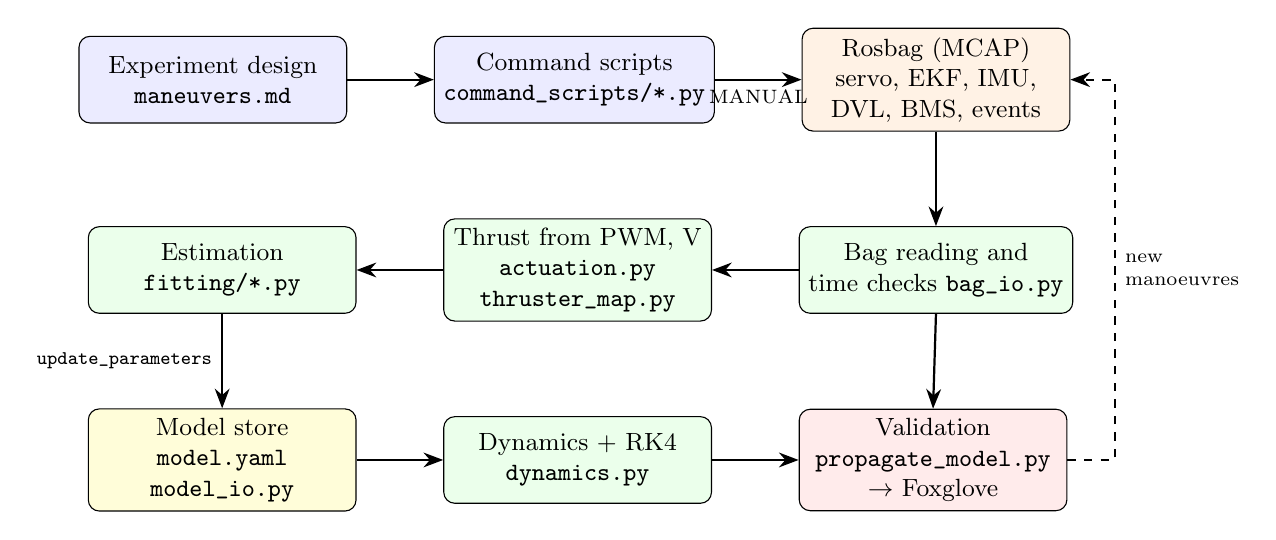
\begin{tikzpicture}[
  node distance=6mm and 11mm,
  box/.style={draw,rounded corners,align=center,font=\small,minimum width=34mm,minimum height=11mm,fill=#1},
  box/.default=white,
  arr/.style={-{Stealth[length=2.5mm]},thick}]
\node[box=blue!8] (design) {Experiment design\\\file{maneuvers.md}};
\node[box=blue!8,right=of design] (cmd) {Command scripts\\\file{command_scripts/*.py}};
\node[box=orange!10,right=of cmd] (bag) {Rosbag (MCAP)\\servo, EKF, IMU,\\DVL, BMS, events};
\node[box=green!8,below=12mm of bag] (io) {Bag reading and\\time checks \file{bag_io.py}};
\node[box=green!8,left=of io] (act) {Thrust from PWM, V\\\file{actuation.py}\\\file{thruster_map.py}};
\node[box=green!8,left=of act] (fit) {Estimation\\\file{fitting/*.py}};
\node[box=yellow!15,below=12mm of fit] (yaml) {Model store\\\file{model.yaml}\\\file{model_io.py}};
\node[box=green!8,right=of yaml] (dyn) {Dynamics + RK4\\\file{dynamics.py}};
\node[box=red!8,right=of dyn] (val) {Validation\\\file{propagate_model.py}\\$\to$ Foxglove};
\draw[arr] (design) -- (cmd);
\draw[arr] (cmd) -- node[below,font=\scriptsize]{MANUAL} (bag);
\draw[arr] (bag) -- (io);
\draw[arr] (io) -- (act);
\draw[arr] (act) -- (fit);
\draw[arr] (fit) -- node[left,font=\scriptsize]{\code{update_parameters}} (yaml);
\draw[arr] (yaml) -- (dyn);
\draw[arr] (dyn) -- (val);
\draw[arr] (io.south) -- (val.north);
\draw[arr,dashed] (val.east) -- ++(6mm,0) |- node[right,pos=0.25,font=\scriptsize,align=left]{new\\manoeuvres} (bag.east);
\end{tikzpicture}
\caption{Stages of the system identification pipeline in \file{scripts/sysid} and the files
that implement them. Arrows indicate data flow; the dashed arrow indicates the iteration
from validation back to new experiments.}
\label{fig:pipeline}
\end{figure}
\FloatBarrier

\begin{table}[htbp]
\centering
\caption{Implementation status of each pipeline stage on \file{feature/sysid}.}
\label{tab:status}
\small
\begin{tabularx}{\textwidth}{@{}l l X@{}}
\toprule
Stage & File(s) & Status \\
\midrule
Manoeuvre catalogue & \file{maneuvers.md} & Written; locations and bags still to be added \\
Command scripts & \file{command_scripts/} & Surge steps (200--500) and coast-down (400) with event markers \\
Model store & \file{model.yaml}, \file{model_io.py} & Diagonal schema for surge, sway, heave, pitch and yaw (sway, heave and $B$ added, roll removed 15 Oct); every coefficient still \code{null} \\
Surge dynamics & \file{dynamics.py} & 1-DOF surge, RK4, steady state; tested against closed forms \\
Thrust map & \file{thruster_map.py}, \file{actuation.py} & T500 PWM $\times$ voltage table on the surge channel; other channels NaN \\
Bag I/O & \file{bag_io.py} & Reads EKF, servo, BMS voltage; timestamp checks; augmented-bag writer \\
Validation & \file{validation/propagate_model.py} & Free-run and re-init propagation, baseline, summary, NavSatFix \\
Estimation & \file{fitting/coupling_check.py} & Equation-error surge fit plus coupling screen; the \code{fit_*.py} scripts are placeholders \\
Synthetic test bench & \file{simulation/synth_bag.py} & Ground-truth bags with known coefficients, delays and noise (added 14 Oct) \\
Tests & \file{tests/} & 32 tests, all passing (24 in the first edition) \\
\bottomrule
\end{tabularx}
\end{table}
\FloatBarrier

\begin{revised}[title=Revised 14 October 2026]
The rows ``Synthetic test bench'' and ``Tests'' of \cref{tab:status} were updated. The synthetic
test bench is described in \cref{ch:synthetic}.

\textbf{15 October 2026.} The row ``Model store'' said ``schema complete'' in the first edition.
That was not true: sway, heave and buoyancy had no slots. They were added (\cref{sec:model-schema}),
and roll was removed from the model (\cref{sec:no-roll}).
\end{revised}

\section{How these notes are organised}

The chapters follow the logical dependency order rather than the order in which the code
was written:
\begin{itemize}
  \item \Cref{ch:frames,ch:fossen,ch:symmetry} cover the physics: frames, the 6-DOF equation, and why the
        vehicle's symmetry allows one axis to be identified at a time.
  \item \Cref{ch:surge,ch:actuation,ch:integration} cover the model as implemented: the surge equation,
        the thrust map, and the integrator.
  \item \Cref{ch:maneuvers,ch:timing} cover how good data is obtained: manoeuvre design and timing.
  \item \Cref{ch:estimation,ch:coupling} cover how parameters are extracted from data.
  \item \Cref{ch:validation} covers how a model is judged, and \cref{ch:status} lists what is open.
\end{itemize}
Each chapter ends with a few questions. The answers are in \cref{app:answers}.
\Cref{app:codemap} is a file-by-file reference.

\begin{keyidea}
The single most important idea in the whole pipeline is \emph{error attribution}. Every design
decision (one axis at a time, open-loop commands, measured delays, free-run validation, a
coupling check) exists so that, when the model disagrees with the data, it can be told
\emph{which} coefficient is wrong and \emph{why}.
\end{keyidea}

\begin{questions}
\begin{enumerate}
  \item Why is the deployed power law $u = 0.780\,\mathrm{sign}(c)|c|^{0.964}$ a black-box
        model, and which physical effect can it not represent?
  \item Name one advantage of a grey-box model over a black-box model for a vehicle that
        will later be operated outside the conditions it was tested in.
\end{enumerate}
\end{questions}

\chapter{Frames, kinematics and notation}
\label{ch:frames}

\section{The two frames that matter}

Two reference frames are needed to describe a vehicle:
\begin{itemize}
  \item a \emph{world} frame fixed to the Earth (\code{odom}), in which position and attitude
        $\vect{\eta} = [x, y, z, \phi, \theta, \psi]^\top$ are expressed;
  \item a \emph{body} frame fixed to the vehicle (\code{base_link}), in which the velocities
        $\vect{\nu} = [u, v, w, p, q, r]^\top$ and the forces $\vect{\tau}$ are expressed.
\end{itemize}
The equations of motion are written in the body frame because the inertia, the added mass
and the damping are constant there. A thruster always pushes along the same body axis,
and the drag of a forward-moving hull always opposes body-forward motion.

\subsection{FLU/ENU (POLARIS) versus FRD/NED (Fossen)}

Marine textbooks, including Fossen \cite{fossen2011}, use the SNAME convention. The body
axes are Forward--Right--Down (FRD) and the world axes North--East--Down (NED). ROS uses
REP-103: body axes Forward--Left--Up (FLU) and world axes East--North--Up (ENU). POLARIS
follows ROS, because every measured signal already arrives in that convention. The EKF
twist is in \code{base_link}, the IMU is identity-rotated to \code{base_link}, and the DVL is
rotated by its TF. \Cref{fig:frames} compares the two body frames.

\begin{figure}[htbp]
\centering
\begin{subfigure}{0.48\textwidth}
\centering
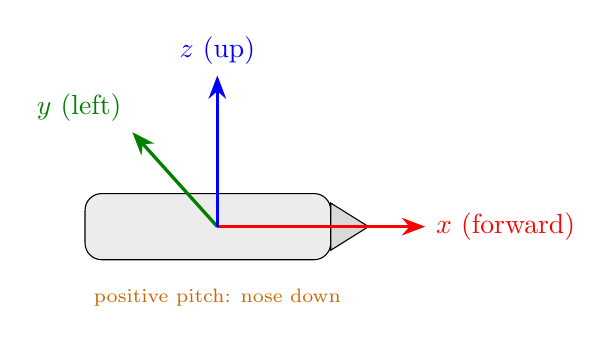
\begin{tikzpicture}[scale=1.2,>=Stealth]
  \draw[fill=gray!15,rounded corners=6pt] (-1.4,-0.35) rectangle (1.2,0.35);
  \draw[fill=gray!30] (1.2,-0.25) -- (1.6,0) -- (1.2,0.25) -- cycle;
  \draw[->,very thick,red] (0,0) -- (2.2,0) node[right]{$x$ (forward)};
  \draw[->,very thick,green!50!black] (0,0) -- (-0.9,1.0) node[above left]{$y$ (left)};
  \draw[->,very thick,blue] (0,0) -- (0,1.6) node[above]{$z$ (up)};
  \node[orange!80!black,font=\scriptsize] at (0,-0.75) {positive pitch: nose down};
\end{tikzpicture}
\caption{FLU (\code{base_link}, REP-103)}
\end{subfigure}\hfill
\begin{subfigure}{0.48\textwidth}
\centering
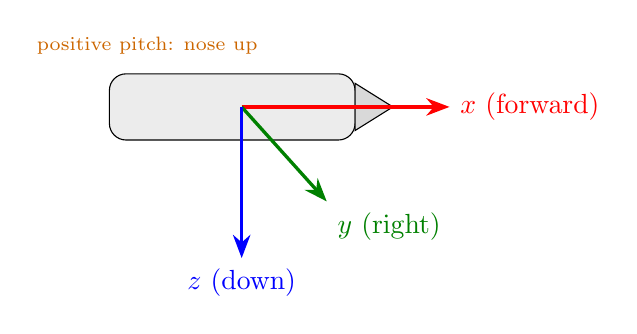
\begin{tikzpicture}[scale=1.2,>=Stealth]
  \draw[fill=gray!15,rounded corners=6pt] (-1.4,-0.35) rectangle (1.2,0.35);
  \draw[fill=gray!30] (1.2,-0.25) -- (1.6,0) -- (1.2,0.25) -- cycle;
  \draw[->,very thick,red] (0,0) -- (2.2,0) node[right]{$x$ (forward)};
  \draw[->,very thick,green!50!black] (0,0) -- (0.9,-1.0) node[below right]{$y$ (right)};
  \draw[->,very thick,blue] (0,0) -- (0,-1.6) node[below]{$z$ (down)};
  \node[orange!80!black,font=\scriptsize] at (-1.0,0.65) {positive pitch: nose up};
\end{tikzpicture}
\caption{FRD (Fossen, SNAME, MAVLink)}
\end{subfigure}
\caption{Body-fixed axes in the FLU convention used by POLARIS and in the FRD convention
used by Fossen, with the sense of positive pitch rate $q$ in each.}
\label{fig:frames}
\end{figure}
\FloatBarrier

The two body frames differ by a rotation of \qty{180}{\degree} about $x$:
$\vect{S} = \mathrm{diag}(1,-1,-1)$. This maps $(u,v,w)\mapsto(u,-v,-w)$ and
$(p,q,r)\mapsto(p,-q,-r)$. It is a proper rotation (determinant $+1$), so cross products,
and therefore the whole Newton--Euler machinery, keep their form.

\begin{keyidea}
\textbf{Pitch is positive nose-down in FLU.} The right-hand rule about $+y$, which points
\emph{left}, turns the nose \emph{down}. This is the opposite of FRD, where $+y$ points
right and positive pitch is nose up. The allocation comments in \file{model.yaml} rely on
this: a rear vertical thruster that pushes up produces a positive pitch moment.
\end{keyidea}

\section{Kinematics}

The velocity in the world frame follows from the body velocity through the kinematic
transformation \cite[ch.~2]{fossen2011}:
\begin{equation}
  \dot{\vect{\eta}} = \vect{J}(\vect{\eta})\,\vect{\nu},
  \qquad
  \vect{J}(\vect{\eta}) = \begin{bmatrix} \vect{R}(\vect{\Theta}) & \vect{0} \\ \vect{0} & \vect{T}(\vect{\Theta}) \end{bmatrix},
  \label{eq:kinematics}
\end{equation}
with the ZYX (yaw--pitch--roll) rotation $\vect{R} = \vect{R}_z(\psi)\vect{R}_y(\theta)\vect{R}_x(\phi)$
and the Euler-rate transformation $\vect{T}$. The formula is the same in FLU/ENU and in
FRD/NED. Only the meaning of the angles changes: in ENU, $\psi$ is measured
counter-clockwise from East.

The propagation script needs only the planar part. With roll and pitch small, the
horizontal position rate is
\begin{equation}
\begin{aligned}
  \dot x &= u\cos\psi - v\sin\psi, \\
  \dot y &= u\sin\psi + v\cos\psi.
\end{aligned}
\label{eq:planar-kin}
\end{equation}

\begin{incode}
\Cref{eq:planar-kin} is exactly the position update inside \code{propagate()} in
\file{validation/propagate_model.py}: \code{pos[0] += h*(c*u - s*v_sub)} and
\code{pos[1] += h*(s*u + c*v_sub)}, with $u$ from the model and $v$, $\psi$ from the EKF.
The Euler angles are extracted in \file{bag_io.py} with
\code{Rotation.from_quat(q).as_euler("xyz")}. Lower-case \code{"xyz"} means
\emph{extrinsic} rotations about fixed axes, which is the same rotation as intrinsic ZYX, so
the result is (roll, pitch, yaw) in the standard aerospace sense.
\end{incode}

\section{Converting coefficients from the literature}

Literature coefficients, such as the BlueROV2 values in \file{dummy_bluerov2_heavy.yaml}
\cite{vonbenzon2022}, are given in FRD. Under the reflection $\vect{S}$ each velocity component
either keeps its sign ($u$, $p$) or flips it ($v$, $w$, $q$, $r$), and the same holds for the
corresponding force component ($X$, $K$ keep, $Y$, $Z$, $M$, $N$ flip). A coefficient
$A_{ab} = \partial A/\partial b$ relates force component $A$ to velocity component $b$, so
it transforms as
\begin{equation}
  A_{ab}^\mathrm{FLU} = s_A\,s_b\,A_{ab}^\mathrm{FRD}, \qquad s \in \{+1, -1\}.
  \label{eq:coef-flip}
\end{equation}

\begin{keyidea}
A coefficient changes sign exactly when \emph{one} of its two indices flips.
\begin{itemize}[nosep]
  \item $X_q$: $X$ keeps, $q$ flips $\Rightarrow$ sign changes.
  \item $Y_r$: both flip $\Rightarrow$ unchanged.
  \item Diagonal terms ($\Xud$, $X_u$, $N_r$, \dots): the same index twice $\Rightarrow$ \textbf{never} change.
\end{itemize}
The surge model in this repository uses only diagonal terms, so the BlueROV2 values were
copied without any sign change apart from the added-mass convention in \cref{sec:addedmass}.
\end{keyidea}

The rule that was adopted is to never copy component tables from Fossen and flip signs by hand.
Every term should instead be built from its vector definition with FLU/ENU inputs. The restoring
vector in \cref{sec:restoring} is the example where this matters most.

\begin{caution}
\file{scripts/custom_frame_helper.py} computes the cross products $\vect{r}_i\times\vect{d}_i$
correctly in FLU, but its \emph{output columns} apply $\text{roll}=+\tau_x$,
$\text{pitch}=-\tau_y$, $\text{yaw}=-\tau_z$, which converts FLU to FRD for ArduSub. The
allocation in \file{model.yaml} uses the raw FLU cross products, not those columns. The
command topic \code{/pixhawk/manual_control} is MAVLink FRD, a third convention handled
by the bridge. It concerns the command scripts only, not the model.
\end{caution}

\begin{questions}
\begin{enumerate}
  \item A paper lists $N_v = \qty{-2.0}{\newton\second}$ in FRD. What is its value in FLU?
  \item Why can $\Xud$, $X_u$ and $\Xuu$ be copied from an FRD paper without change?
  \item The EKF publishes twist in \code{base_link} and pose in \code{odom}. Which of the two
        is needed to evaluate the drag force, and which to compare predicted and measured tracks?
\end{enumerate}
\end{questions}

\chapter{Fossen's six-degree-of-freedom model}
\label{ch:fossen}

The starting point of \file{maneuvers.md} is the manoeuvring model of Fossen
\cite[ch.~6--7]{fossen2011}, written with the velocity relative to the water
$\vect{\nu}_r = \vect{\nu} - \vect{\nu}_c$:
\begin{equation}
  \underbrace{(\vect{M}_\mathrm{RB} + \vect{M}_\mathrm{A})\,\dot{\vect{\nu}}_r}_{\text{inertia}}
  + \underbrace{\vect{C}_\mathrm{RB}(\vect{\nu})\vect{\nu} + \vect{C}_\mathrm{A}(\vect{\nu}_r)\vect{\nu}_r}_{\text{Coriolis--centripetal}}
  + \underbrace{\vect{D}(\vect{\nu}_r)\,\vect{\nu}_r}_{\text{damping}}
  + \underbrace{\vect{g}(\vect{\eta})}_{\text{restoring}}
  = \vect{\tau}_\mathrm{thrust} + \vect{\tau}_\mathrm{dist}.
  \label{eq:fossen}
\end{equation}
This chapter takes the terms one at a time and explains what physical effect each
represents, how big it is, and which coefficient in \file{model.yaml} belongs to it.

\section{Rigid-body dynamics}

Newton's and Euler's laws about the centre of mass, written in a rotating body frame, read
\begin{align}
  m\,(\dot{\vect{v}} + \vect{\omega}\times\vect{v}) &= \vect{f}, \label{eq:newton}\\
  \vect{I}\,\dot{\vect{\omega}} + \vect{\omega}\times(\vect{I}\vect{\omega}) &= \vect{m}, \label{eq:euler}
\end{align}
with $\vect{v} = [u,v,w]^\top$ and $\vect{\omega} = [p,q,r]^\top$. The cross products are
not forces. They appear because the frame in which $\dot{\vect{v}}$ is measured rotates
with the vehicle. In matrix form, \cref{eq:newton,eq:euler} become
$\vect{M}_\mathrm{RB}\dot{\vect{\nu}} + \vect{C}_\mathrm{RB}(\vect{\nu})\vect{\nu}$. The surge
row of \eqref{eq:newton} is
\begin{equation}
  m\,(\dot u - v r + w q) = X .
  \label{eq:surge-rb}
\end{equation}
Both $v r$ and $w q$ are products of two components that flip together under the FRD/FLU
reflection, so \eqref{eq:surge-rb} reads identically in both conventions. The origin of
\code{base_link} lies at the centre of mass (per the DVL launch file), so the lever-arm terms
that Fossen carries for an offset centre of gravity vanish.

\section{Added mass}
\label{sec:addedmass}

When a body accelerates through a fluid, it must also accelerate some of the surrounding
fluid. The fluid's kinetic energy is a quadratic form of the body velocity,
$T_\mathrm{A} = \tfrac12\vect{\nu}^\top\vect{M}_\mathrm{A}\vect{\nu}$, and the energy needed to
build it up appears to the body as extra inertia \cite{newman1977}. For a sphere the added
mass is exactly half the displaced fluid mass. For an ROV-shaped body it is typically
\SIrange{30}{100}{\percent} of the dry mass in translation. In the BlueROV2 data,
$-\Xud = \qty{6.36}{\kilogram}$ against $m = \qty{13.5}{\kilogram}$.

The SNAME notation writes added mass as a \emph{hydrodynamic derivative}:
$\Xud = \partial X/\partial\dot u$, the change of hydrodynamic surge force per unit surge
acceleration. Accelerating forward causes the fluid to push \emph{back}, so $\Xud < 0$, and
moving it to the left-hand side gives
\begin{equation}
  (m - \Xud)\,\dot u = \dots, \qquad \mtot \coloneqq m - \Xud > m.
  \label{eq:mtot}
\end{equation}

\begin{caution}
Sign conventions differ between the code and much of the literature.
\begin{itemize}[nosep]
  \item \textbf{Added mass} is stored with Fossen's sign: \code{X_udot} is \emph{negative}.
        Tables that list a positive magnitude (as von Benzon et al.\ \cite{vonbenzon2022} do)
        must be negated when entered.
  \item \textbf{Damping} is stored as a positive \emph{magnitude}: \code{X_u} $> 0$, and the
        force is $-X_u u$. Fossen writes the force as $+X_u u$ with $X_u < 0$.
\end{itemize}
\code{SurgeParams.__post_init__} in \file{dynamics.py} rejects $\mtot \le 0$. That catches a
wrongly signed added mass that is large enough to make the inertia non-positive. A smaller
sign error does not violate the check: it gives a valid but wrong $\mtot < m$.
\end{caution}

\subsection{Added-mass Coriolis terms}

The added mass also contributes Coriolis-like terms. The fluid momentum
$\vect{p}_\mathrm{A} = \vect{M}_\mathrm{A}\vect{\nu}$ is carried along by the rotating frame
in the same way as the body momentum (Kirchhoff's equations \cite{newman1977}). For a diagonal
$\vect{M}_\mathrm{A} = -\mathrm{diag}(\Xud, Y_{\dot v}, Z_{\dot w}, \dots)$ the translational
part of the fluid's reaction is $-\vect{\omega}\times\vect{p}_\mathrm{A}$, whose $x$
component is
\begin{equation}
  -\bigl(q\,(-Z_{\dot w}w) - r\,(-Y_{\dot v}v)\bigr) = Z_{\dot w}\,wq - Y_{\dot v}\,vr .
\end{equation}
Adding this to \eqref{eq:surge-rb} gives the classical surge equation with its two
velocity-product terms:
\begin{equation}
  \boxed{\;(m - \Xud)\,\dot u \;-\; (m - Y_{\dot v})\,v r \;+\; (m - Z_{\dot w})\,w q \;=\; X_\mathrm{hydro} + X_\mathrm{thrust}\;}
  \label{eq:surge-full}
\end{equation}
With the BlueROV2 numbers $m - Y_{\dot v} = 13.5 + 7.12 = \qty{20.6}{\kilogram}$. A vehicle
that turns at $r = \qty{0.5}{\radian\per\second}$ while side-slipping at
$v = \qty{0.1}{\meter\per\second}$ therefore experiences about \qty{1}{\newton} of apparent
surge force. That is small but not negligible against a thrust of a few newtons. These are
exactly the \code{v*r} and \code{w*q} candidates in the coupling check (\cref{ch:coupling}),
and the synthetic test in \file{tests/test_coupling_check.py} injects $k\,vr$ with
$k = -20$ for this reason.

\section{Damping}

Hydrodynamic damping has several physical sources: skin friction, pressure (form) drag from
flow separation, vortex shedding, and lift on appendages. For manoeuvring at low speed it is
modelled as the sum of a linear and a quadratic part \cite[sec.~6.4]{fossen2011}:
\begin{equation}
  \vect{D}(\vect{\nu})\vect{\nu} = \vect{D}_l\,\vect{\nu} + \vect{D}_n(\vect{\nu})\,\vect{\nu},
  \qquad
  \text{surge: } \; X_\mathrm{hydro} = -X_u\,u - \Xuu\,|u|\,u .
  \label{eq:damping}
\end{equation}
\begin{itemize}
  \item The \emph{quadratic} term is the familiar drag law $F = \tfrac12\rho C_D A\,|u|u$
        at high Reynolds number. The form $|u|u$ rather than $u^2$ makes the force odd in
        $u$, so drag always opposes the motion.
  \item The \emph{linear} term dominates at very low speed (laminar skin friction, and
        effects such as wave radiation at the surface). Its absolute size is small. It
        matters mainly because it sets the decay rate near zero speed.
\end{itemize}
Off-diagonal damping terms are neglected by assumption. Their absence is part of what the
coupling check tests.

\section{Restoring forces}
\label{sec:restoring}

Gravity $W = mg$ acts at the centre of gravity $\vect{r}_g$ and buoyancy
$B = \rho g\nabla$ at the centre of buoyancy $\vect{r}_b$. In the ENU world frame gravity
points along $-z$. Building the restoring vector from vectors rather than from Fossen's NED
table gives the correct signs automatically:
\begin{equation}
  \vect{f}_g = \vect{R}^\top\begin{bmatrix}0\\0\\-W\end{bmatrix}, \quad
  \vect{f}_b = \vect{R}^\top\begin{bmatrix}0\\0\\B\end{bmatrix}, \quad
  \vect{g}(\vect{\eta}) = -\begin{bmatrix} \vect{f}_g + \vect{f}_b \\
     \vect{r}_g\times\vect{f}_g + \vect{r}_b\times\vect{f}_b \end{bmatrix}.
  \label{eq:restoring}
\end{equation}

\paragraph{Small-angle pitch stiffness.} Take $\vect{r}_g = \vect{0}$,
$\vect{r}_b = [0, 0, \overline{BG}]^\top$ (buoyancy \emph{above} gravity, so $z_b > 0$ in FLU,
whereas Fossen's NED tables have it negative) and a pure pitch $\vect{R} = \vect{R}_y(\theta)$.
Then $\vect{f}_b = [-B\sin\theta,\;0,\;B\cos\theta]^\top$ and
\begin{equation}
  \vect{r}_b\times\vect{f}_b = [\,0,\; -B\,\overline{BG}\sin\theta,\; 0\,]^\top
  \;\;\Rightarrow\;\;
  g_\theta = B\,\overline{BG}\sin\theta \approx M_\theta\,\theta,
  \quad M_\theta = B\,\overline{BG}.
  \label{eq:pitch-stiffness}
\end{equation}
The moment opposes the tilt, so the vehicle is statically stable. Roll gives the same result,
$K_\phi = B\,\overline{BG}$ (for $W = B$). The dummy file derives $K_\phi = M_\theta =
\qty{131.6}{\newton}\times\qty{0.01}{\meter} = \qty{1.316}{\newton\meter\per\radian}$ in
exactly this way.

\paragraph{Trim angles.} If the centre of buoyancy is not exactly above the centre of
gravity, the vehicle floats tilted at $\phi_0, \theta_0$, and the restoring torque pulls
towards that attitude rather than towards level: $g_\theta \approx M_\theta(\theta-\theta_0)$.
This is why \file{model.yaml} carries \code{phi_0} and \code{theta_0}, to be measured from
a still, powered-down float. (Since 15 October 2026 only \code{theta_0}; roll is not
modelled, \cref{sec:no-roll}.)

\paragraph{Yaw.} No restoring moment exists in yaw, because buoyancy and gravity are both
vertical. Yaw is a pure integrator with damping and never oscillates back. This is why the
static tests in \file{maneuvers.md} cover roll and pitch only.

\paragraph{Net buoyancy in surge.} If $W \ne B$, the translational part of
\eqref{eq:restoring} gives a surge component $(W - B)\sin\theta$ whenever the vehicle is
pitched. This is the \code{sin(pitch)} candidate of the coupling check.

\section{The model schema in \file{model.yaml}}
\label{sec:model-schema}

\begin{revised}[title={New section, added 15 October 2026}]
Until this revision \file{model.yaml} had slots for surge, roll, pitch and yaw only. The sway
and heave coefficients $Y_{\dot v}$, $Y_v$, $Y_{v|v|}$, $Z_{\dot w}$, $Z_w$, $Z_{w|w|}$ and the
buoyancy $B$ were added, so that the file now holds the complete diagonal model of
\eqref{eq:fossen}. No code reads the new entries yet.

\textbf{Later the same day} roll was removed from the model (\cref{sec:no-roll}): the slots
$I_{xx}$, $K_{\dot p}$, $K_p$, $K_{p|p|}$, $K_\phi$ and $\phi_0$ were deleted, the roll row of
\cref{tab:model-schema} was changed, and the equations below were written without roll.
\file{model.yaml} now has 21 parameters.
\end{revised}

With the port--starboard symmetry of \cref{ch:symmetry} and the off-diagonal terms neglected,
\eqref{eq:fossen} is fully determined by the parameters in \cref{tab:model-schema}. The
Coriolis--centripetal matrices $\vect{C}_\mathrm{RB}$ and $\vect{C}_\mathrm{A}$ need no
parameters of their own: they are built from $m$, the inertias and the same added-mass
derivatives \cite{fossen2011}. With the abbreviations
$m_{11} = m - \Xud$, $m_{22} = m - Y_{\dot v}$, $m_{33} = m - Z_{\dot w}$ and the roll
rate $p$ set to zero (\cref{sec:no-roll}), the translational equations are
\begin{align}
  m_{11}\,\dot u &= \tau_X - X_u\,u - \Xuu\,|u|\,u + (W - B)\sin\theta
                    + m_{22}\,v r - m_{33}\,w q, \label{eq:diag-surge}\\
  m_{22}\,\dot v &= \tau_Y - Y_v\,v - Y_{v|v|}\,|v|\,v + (B - W)\sin\phi\cos\theta
                    - m_{11}\,u r, \label{eq:diag-sway}\\
  m_{33}\,\dot w &= \tau_Z - Z_w\,w - Z_{w|w|}\,|w|\,w + (B - W)\cos\phi\cos\theta
                    + m_{11}\,u q. \label{eq:diag-heave}
\end{align}
The restoring terms follow from \eqref{eq:restoring} in the same way as
\eqref{eq:pitch-stiffness}: $\vect{R}^\top[0,0,1]^\top = [-\sin\theta,\ \sin\phi\cos\theta,\
\cos\phi\cos\theta]^\top$, and the net force on the vehicle is $(B-W)$ times this vector.
The roll angle $\phi$ is taken from the EKF; it is a measured input, not a state. Pitch and
yaw follow in the same way with $M_\theta(\theta-\theta_0)$ as the pitch restoring moment and
none in yaw. The Coriolis products in \eqref{eq:diag-surge}--\eqref{eq:diag-heave} are the
components of $-\vect{\omega}\times(\vect{M}_t\vect{v})$ with
$\vect{M}_t = \mathrm{diag}(m_{11}, m_{22}, m_{33})$. This form follows from vectors and holds
in any right-handed body frame, including FLU.

\begin{table}[htbp]
\centering
\caption{Parameters of the diagonal model in \file{model.yaml}, grouped by degree of freedom,
with the inertia, damping and restoring entries of each.}
\label{tab:model-schema}
\small
\begin{tabularx}{\textwidth}{@{}l l X l@{}}
\toprule
DOF & Inertia & Damping (\code{damping_linear}, \code{damping_quadratic}) & Restoring \\
\midrule
Surge & $m$, $\Xud$ & $X_u$, $\Xuu$ & via $W - B$ \\
Sway  & $m$, $Y_{\dot v}$ & $Y_v$, $Y_{v|v|}$ & via $W - B$ \\
Heave & $m$, $Z_{\dot w}$ & $Z_w$, $Z_{w|w|}$ & $B$ (with $W = mg$) \\
Roll  & \multicolumn{3}{l}{not modelled; $\phi$ and $p$ from the EKF (\cref{sec:no-roll})} \\
Pitch & $I_{yy}$, $M_{\dot q}$ & $M_q$, $M_{q|q|}$ & $M_\theta$, $\theta_0$ \\
Yaw   & $I_{zz}$, $N_{\dot r}$ & $N_r$, $N_{r|r|}$ & none \\
\bottomrule
\end{tabularx}
\end{table}
\FloatBarrier

\paragraph{What the schema deliberately leaves out.}
\begin{itemize}
  \item \textbf{Centre of gravity and centre of buoyancy.} They enter only through
        $M_\theta$ and $\theta_0$, which are lumped and measured directly.
        Keeping both $\vect{r}_b$ and $M_\theta$ would describe the same physics twice.
  \item \textbf{Off-diagonal terms} such as $X_{\dot w}$, $M_{\dot u}$ or $Z_q$. They are added
        only if the combined-axes runs leave a residual the diagonal model cannot explain
        (\cref{ch:symmetry}).
  \item \textbf{Water current and tether.} These are treated as disturbances, not model
        parameters.
\end{itemize}

\begin{caution}
$B - W$ is a small difference of two large forces. Weighing the dry vehicle ($m$) and computing
$B$ from the displaced volume will not give it to useful accuracy. A direct measurement of the
net buoyancy, for example with a spring scale on the submerged vehicle, is preferable. If
POLARIS operates at the surface, heave restoring is dominated by the waterplane stiffness
$\rho g A_\mathrm{wp}$, which has no slot yet.
\end{caution}

\subsection{Roll is not modelled}
\label{sec:no-roll}

\begin{revised}[title={New subsection, added 15 October 2026}]
The decision to drop roll and the evidence from the recorded bags. The roll statistics were
computed with a throw-away script over the EKF of the existing recordings; they are not
reproduced by \file{gen_figdata.py}.
\end{revised}

POLARIS is passively roll-stable: the centre of buoyancy lies above the centre of gravity,
and the restoring moment $K_\phi\phi$ of \eqref{eq:pitch-stiffness} pulls it back upright.
Roll is never commanded during identification. The roll equation is therefore dropped, and so
is every Coriolis product that contains the roll rate $p$. \Cref{tab:roll-terms} lists them.
As a consequence $I_{xx}$ and $K_{\dot p}$ no longer appear in any remaining equation, and
the slots $I_{xx}$, $K_{\dot p}$, $K_p$, $K_{p|p|}$, $K_\phi$, $\phi_0$ were removed from
\file{model.yaml}.

\begin{table}[htbp]
\centering
\caption{Coriolis--centripetal products containing the roll rate $p$ that are removed by not
modelling roll, from $-\vect{\omega}\times(\vect{M}_t\vect{v})$ and
$-\vect{\omega}\times(\vect{I}_t\vect{\omega}) - \vect{v}\times(\vect{M}_t\vect{v})$, with
$I_{11} = I_{xx} - K_{\dot p}$, $I_{22} = I_{yy} - M_{\dot q}$, $I_{33} = I_{zz} - N_{\dot r}$.}
\label{tab:roll-terms}
\small
\begin{tabular}{@{}lll@{}}
\toprule
Equation & Removed term & Physical meaning \\
\midrule
Sway  & $+m_{33}\,w p$ & Heave velocity turned into sway by rolling \\
Heave & $-m_{22}\,v p$ & Sway velocity turned into heave by rolling \\
Pitch & $-(I_{11} - I_{33})\,p r$ & Gyroscopic pitch moment of combined roll and yaw rates \\
Yaw   & $-(I_{22} - I_{11})\,p q$ & Gyroscopic yaw moment of combined roll and pitch rates \\
Roll  & whole equation & Roll inertia, damping and stiffness \\
\bottomrule
\end{tabular}
\end{table}
\FloatBarrier

\paragraph{Surge is unaffected.} The diagonal surge equation \eqref{eq:diag-surge} contains no
$p$ and no $\phi$. Dropping roll changes nothing in the surge work of \cref{ch:surge}.

\paragraph{The roll angle is still used.} Dropping the roll \emph{dynamics} is not the same as
setting $\phi = 0$. The angle enters the restoring terms of \eqref{eq:diag-sway} and
\eqref{eq:diag-heave} and the kinematics $\vect{J}(\vect{\eta})$ that turn body velocities into
world positions. The EKF provides $\phi$ at no cost, so it is replayed there, exactly as
\code{dofs.roll: measured} already did for the propagation (\cref{ch:symmetry}). Setting
$\phi = 0$ would discard information without simplifying anything.

\paragraph{Evidence from the recordings.} \Cref{tab:roll-evidence} summarises the EKF roll angle
of the existing bags, restricted to samples with $|u| > \qty{0.3}{\meter\per\second}$.
``Straight'' means $|r| < \qty{3}{\degree\per\second}$, ``turning'' means
$|r| > \qty{10}{\degree\per\second}$.

\begin{table}[htbp]
\centering
\caption{EKF roll angle in the existing recordings while moving: median roll, 95th percentile of
the deviation from the median on straight segments and in turns, and the dominant frequency of
the roll signal.}
\label{tab:roll-evidence}
\small
\begin{tabular}{@{}lcccc@{}}
\toprule
Bag & Median & $|\Delta\phi|_{95}$ straight & $|\Delta\phi|_{95}$ turning & Peak frequency \\
 & (\unit{\degree}) & (\unit{\degree}) & (\unit{\degree}) & (\unit{\hertz}) \\
\midrule
\file{zermatt_rectangle_01} & $-2.0$ & 2.0 & 3.9 & 0.56 \\
\file{zermatt_rectangle_04} & $-2.2$ & 2.1 & -- & 0.03 \\
\file{zermatt_rectangle_06} & $-2.1$ & 2.4 & -- & 0.03 \\
\file{zermatt_rectangle_07} & $-2.2$ & 2.0 & -- & 0.06 \\
\file{zermatt_rectangle_08} & $-2.0$ & 2.1 & 3.4 & 0.63 \\
\file{zermatt_grid_01}      & $-0.6$ & 3.1 & -- & 0.03 \\
\file{zermatt_grid_02}      & $-0.6$ & 6.7 & 88 & 0.03 \\
\file{aut_no_z_surface_big_40_grid_03} & $-1.1$ & 14.2 & 5.5 & 0.56 \\
\bottomrule
\end{tabular}
\end{table}
\FloatBarrier

Three observations follow from \cref{tab:roll-evidence}.
\begin{enumerate}
  \item In the Zermatt rectangle runs roll stays within about \qty{2}{\degree} on straight
        segments and about \qty{4}{\degree} in turns. Turn-induced heel is small, so the
        removed terms of \cref{tab:roll-terms} are small there as well.
  \item In the June surface run, roll reaches \qty{14}{\degree} on \emph{straight} segments, with
        a peak at \qty{0.56}{\hertz}. That is wave-induced roll, not a consequence of
        manoeuvring. A roll model would not predict it either, because the wave forcing is not
        measured. The roll rate there reaches about \qty{43}{\degree\per\second} (95th percentile), so the removed
        sway and heave products are no longer negligible. Such bags should not be used for sway
        or heave fits.
  \item The turning value of \file{zermatt_grid_02} (\qty{88}{\degree}) and the large maxima in
        some bags are almost certainly handling or recovery while the EKF was running, not
        manoeuvring. This was not checked further. In every bag the vehicle moves faster than
        \qty{0.3}{\meter\per\second} only \qtyrange{2}{42}{\percent} of the time.
\end{enumerate}
The consistent median of about \qty{-2}{\degree} in the rectangle runs is either a real list of
the vehicle or an IMU mounting offset. It does not matter for the model, because $\phi$ is
replayed from the EKF.

\begin{caution}
The decision is sound as long as (i) bags used for sway, heave or yaw fits have small roll, for
example $|\Delta\phi|_{95} < \qty{5}{\degree}$; (ii) ArduSub is not commanding roll during the
runs, since the flight mode may stabilise roll actively through the rear vertical pair; and
(iii) the combined surge--yaw runs of \cref{ch:symmetry} do not leave a residual correlated with
$p$. If any of these fails, the six slots can be restored from git history.
\end{caution}

\section{Thrust and disturbances}

$\vect{\tau}_\mathrm{thrust}$ is never measured directly. It is reconstructed from the
logged PWM through the thruster map (\cref{ch:actuation}) and the allocation matrix.
$\vect{\tau}_\mathrm{dist}$ collects everything that is not modelled: water current (which
enters through $\vect{\nu}_c$), tether drag, and waves when at the surface. For the
identification these are treated as \emph{nuisance} terms. A slowly varying current or
tether pull looks like a constant force offset, which is why \code{coupling_check.py} fits
an optional \code{offset [N]} regressor.

\begin{questions}
\begin{enumerate}
  \item Show from \eqref{eq:newton} that the surge equation contains $-m\,vr$ and $+m\,wq$.
  \item A colleague enters $\Xud = +\qty{6.36}{\kilogram}$ from a paper into \file{model.yaml}.
        What $\mtot$ results for $m = \qty{13.5}{\kilogram}$, and would
        \code{SurgeParams} reject it?
  \item Why does the restoring vector contain no yaw stiffness?
  \item Where in \file{model.yaml} would a measured $\overline{BG}$ end up?
\end{enumerate}
\end{questions}

\chapter{Symmetry and decoupling}
\label{ch:symmetry}

Identifying all of \eqref{eq:fossen} at once would mean estimating dozens of coefficients
from data in which every axis moves at the same time. The plan in \file{maneuvers.md} is to
identify one axis at a time instead. This chapter explains why that is legitimate and where
it stops being legitimate.

\section{The reflection argument}

POLARIS is (approximately) mirror-symmetric about its $xz$ plane: port and starboard are
mirror images. Consider the reflection $y \mapsto -y$. Under it
\begin{itemize}
  \item the \textbf{longitudinal} variables $u$, $w$, $q$ and forces $X$, $Z$, $M$ are unchanged;
  \item the \textbf{lateral} variables $v$, $p$, $r$ and forces $Y$, $K$, $N$ change sign.
\end{itemize}
A symmetric vehicle cannot tell a manoeuvre from its mirror image, so its equations must be
invariant under the reflection. Consequently:
\begin{keyidea}
A longitudinal force ($X$, $Z$, $M$) can depend on the lateral variables only through
\emph{even} combinations such as $v^2$, $r^2$ or $vr$. A lateral force ($Y$, $K$, $N$)
must be \emph{odd} in the lateral variables, for example $v$, $r$, $ur$ or $uv$.
\end{keyidea}
After linearising about straight-line motion ($v = p = r = 0$), every even combination
vanishes to first order, and the inertia and damping matrices become block-diagonal after
reordering the states:
\begin{equation}
  \vect{M} \;\to\; \begin{bmatrix} \vect{M}_\mathrm{lon} & \vect{0} \\ \vect{0} & \vect{M}_\mathrm{lat} \end{bmatrix},
  \qquad
  \text{lon} = (u, w, q), \quad \text{lat} = (v, p, r).
  \label{eq:blockdiag}
\end{equation}
Surge, heave and pitch form one group, and sway, roll and yaw the other. Exciting surge alone
does not, to first order, produce sway, roll or yaw. Each group can therefore be identified
from its own manoeuvres.

\section{What survives the symmetry}

The decoupling is only \emph{first-order}. Three kinds of coupling remain.
\begin{enumerate}
  \item \textbf{Within a group.} Surge, heave and pitch can still couple to each other, for
        example through off-diagonal added mass $X_{\dot w}$ or $M_{\dot u}$, or through the
        restoring term $(W-B)\sin\theta$.
  \item \textbf{Nonlinear cross-group terms.} The products in \eqref{eq:surge-full} are even in
        the lateral variables, so they are allowed in surge: $-(m-Y_{\dot v})\,vr$. In the
        lateral group the products of a longitudinal and a lateral variable survive, for example the
        sway force $(m-\Xud)\,ur$ and the Munk yaw moment, which is proportional to $(\Xud - Y_{\dot v})\,uv$. This is the
        ``surge--yaw'' coupling of \file{maneuvers.md} section 2.6: turning while moving
        forward.
  \item \textbf{Actuation-level coupling.} Thrusters do not have to respect the hull's symmetry.
        In POLARIS, \code{MOT_1}, the only surge thruster, sits \qty{3}{\centi\meter} above the
        centre of mass. Its line of action therefore produces a pitch moment
        $M = 0.03\,T$, recorded in \file{model.yaml} as the lever \code{0.0300} in the
        \code{pitch} allocation. Because $M$ and $\theta$ are both measured in FLU, where pitch
        is positive nose-down, forward thrust pitches the nose down. In steady state that
        moment is balanced by the restoring torque,
        $\theta_\mathrm{ss} - \theta_0 = 0.03\,T/M_\theta$, so its size depends on the
        still unknown stiffness $M_\theta$. With the dummy BlueROV2 stiffness
        $\qty{1.316}{\newton\meter\per\radian}$ a \qty{20}{\newton} thrust would give
        \qty{0.46}{\radian}. That shows the lever cannot be dismissed until $M_\theta$ has been measured.
\end{enumerate}

\section{Consequences for the plan}

The per-axis plan follows directly from the argument:
\begin{enumerate}
  \item Identify each axis from manoeuvres that excite only that axis. The other axes are
        given to the model as \emph{measured} inputs from the EKF (the \code{dofs:} section of
        \file{model.yaml}).
  \item Validate the per-axis models on holdout runs.
  \item Command two axes together (section 2.6 of \file{maneuvers.md}). If the per-axis models still
        explain the data, coupling is negligible. If a systematic residual remains, fit a
        correction term while leaving the per-axis coefficients untouched.
\end{enumerate}

\begin{revised}[title=Revised 15 October 2026]
Roll is not modelled any more (\cref{sec:no-roll}). The lateral group of the identified model is
therefore $(v, r)$, with $\phi$ and $p$ replayed from the EKF. The symmetry argument is
unaffected: it only states which groups may be identified separately.
\end{revised}

\begin{incode}
The \code{dofs:} block in \file{model.yaml} switches every DOF between \code{modelled} and
\code{measured}. Currently only \code{surge: modelled}; heading, sway, depth and attitude are
replayed from the EKF inside \code{propagate()}. A wrong surge prediction therefore cannot
be blamed on a wrong yaw model. This is error attribution by construction.
\end{incode}

\begin{questions}
\begin{enumerate}
  \item Is a term $X_{vv}\,v^2$ in the surge equation allowed for a port--starboard symmetric
        vehicle? Is $X_v\,v$?
  \item Why does the coupling check include $r^2$ but not $r$ as a natural Fossen term in
        surge? (The code nevertheless tests $r$ as a generic candidate. Why might that still
        be useful?)
  \item Which of the three kinds of surviving coupling would the combined-axes manoeuvre
        (surge and yaw together) excite?
\end{enumerate}
\end{questions}

\chapter{The surge model}
\label{ch:surge}

\section{From six DOFs to one}

Starting from \eqref{eq:surge-full} with the damping \eqref{eq:damping}, the following
assumptions reduce surge to a scalar equation:
\begin{enumerate}
  \item The products $vr$ and $wq$ are small during surge manoeuvres (straight-line runs)
        or are absorbed into the residual. The coupling check tests this assumption.
  \item Pitch stays small, so $(W-B)\sin\theta$ is negligible.
  \item Current and tether are neglected, or absorbed into a constant offset.
  \item The thrust $T$ is known from the PWM and the battery voltage.
\end{enumerate}
This gives the model implemented in \file{dynamics.py}:
\begin{equation}
  \boxed{\;\mtot\,\dot u = T - X_u\,u - \Xuu\,|u|\,u, \qquad \mtot = m - \Xud\;}
  \label{eq:surge}
\end{equation}
Three numbers describe it completely: $\mtot$, $X_u$ and $\Xuu$. These are the three
\code{REQUIRED} keys checked by \file{propagate_model.py} ($m$ and $\Xud$ are stored
separately and combined into $\mtot$).

\section{Steady state}

At constant thrust the acceleration vanishes, and \eqref{eq:surge} becomes a quadratic in
$u_\mathrm{ss}$ (for $T > 0$):
\begin{equation}
  \Xuu\,u_\mathrm{ss}^2 + X_u\,u_\mathrm{ss} - T = 0
  \quad\Rightarrow\quad
  u_\mathrm{ss} = \frac{-X_u + \sqrt{X_u^2 + 4\Xuu T}}{2\Xuu}.
  \label{eq:uss}
\end{equation}
For $T<0$ the result is mirrored, $u_\mathrm{ss}(-T) = -u_\mathrm{ss}(T)$. This is
\code{steady_state_speed()}. The steady state does \emph{not} depend on $\mtot$: mass only
decides how quickly the steady state is reached. \Cref{fig:drag} (left) shows the two damping
contributions for the dummy coefficients. The quadratic part dominates above about
\qty{0.1}{\meter\per\second}, where $\Xuu u = X_u$.

\section{Local time constant}
\label{sec:taueff}

Linearising \eqref{eq:surge} about an operating speed $u_0 > 0$ with $u = u_0 + \delta u$:
\begin{equation}
  \mtot\,\dot{\delta u} = \delta T - (X_u + 2\Xuu u_0)\,\delta u
  \quad\Rightarrow\quad
  \taueff(u_0) = \frac{\mtot}{X_u + 2\Xuu\,|u_0|}.
  \label{eq:taueff}
\end{equation}
At $u_0 = 0$ this is the number quoted in \file{maneuvers.md},
$\mtot/X_u = 19.86/13.7 = \qty{1.45}{\second}$. Because the quadratic damping stiffens rapidly
with speed, the time constant at cruising speed is much shorter (\cref{tab:taueff},
\cref{fig:drag} right).

\begin{table}[htbp]
\centering
\caption{Steady-state speed and local time constant of the surge model at four thrust
levels, for the dummy BlueROV2 coefficients $\mtot = \qty{19.86}{\kilogram}$,
$X_u = \qty{13.7}{\newton\second\per\meter}$, $\Xuu = \qty{141}{\newton\second\squared\per\meter\squared}$.}
\label{tab:taueff}
\begin{tabular}{@{}S[table-format=2.0] S[table-format=1.3] S[table-format=1.3]@{}}
\toprule
{Thrust $T$ / \unit{\newton}} & {$u_\mathrm{ss}$ / \unit{\meter\per\second}} & {$\taueff$ / \unit{\second}} \\
\midrule
0  & 0.000 & 1.450 \\
5  & 0.146 & 0.362 \\
10 & 0.222 & 0.260 \\
20 & 0.331 & 0.185 \\
40 & 0.486 & 0.132 \\
\bottomrule
\end{tabular}
\end{table}
\FloatBarrier

\begin{keyidea}
``The surge time constant'' is not a single number for a quadratically damped vehicle. With
the dummy coefficients it falls from \qty{1.45}{\second} at rest to under
\qty{0.2}{\second} at \qty{0.3}{\meter\per\second}. The delays discussed in \cref{ch:timing}
(\qtyrange{100}{300}{\milli\second}) are compared against the $\taueff$ \emph{at the speed
of the manoeuvre}, which makes them far more significant than the \qty{1.4}{\second} figure
suggests. The real POLARIS value must be checked once $X_u$ and $\Xuu$ are known.
\end{keyidea}

\begin{figure}[htbp]
\centering
\begin{subfigure}{0.48\textwidth}
\centering
\begin{tikzpicture}
\begin{axis}[notes,xlabel={$u$ / \unit{\meter\per\second}},ylabel={Damping force / \unit{\newton}},xmin=0,xmax=0.8,ymin=0]
\addplot[blue,dashed] table[x=u,y=lin]{data/drag.dat};
\addplot[red,dashdotted] table[x=u,y=quad]{data/drag.dat};
\addplot[black] table[x=u,y=tot]{data/drag.dat};
\legend{$X_u u$,$\Xuu u^2$,total}
\end{axis}
\end{tikzpicture}
\caption{Damping force}
\end{subfigure}\hfill
\begin{subfigure}{0.48\textwidth}
\centering
\begin{tikzpicture}
\begin{axis}[notes,xlabel={$u_0$ / \unit{\meter\per\second}},ylabel={$\taueff$ / \unit{\second}},
  xmin=0,xmax=0.8,ymin=0,ymax=1.6]
\addplot[black] table[x=u,y=tau]{data/drag.dat};
\end{axis}
\end{tikzpicture}
\caption{Local time constant \eqref{eq:taueff}}
\end{subfigure}
\caption{Linear, quadratic and total surge damping force, and the local time constant
$\taueff$, as functions of surge speed for the dummy BlueROV2 coefficients.}
\label{fig:drag}
\end{figure}
\FloatBarrier

\section{Closed-form solutions}
\label{sec:closedform}

\Cref{eq:surge} is a first-order nonlinear ODE, but several special cases have closed-form
solutions. They are the backbone of the unit tests and of the manoeuvre design.

\paragraph{Thrust-free, linear damping only.} $\mtot\dot u = -X_u u$ gives an exponential decay:
\begin{equation}
  u(t) = u_0\,e^{-X_u t/\mtot}.
  \label{eq:decay-lin}
\end{equation}

\paragraph{Thrust-free, quadratic damping only.} $\mtot\dot u = -\Xuu u^2$ (for $u>0$) is
separable, $-\mathrm{d}u/u^2 = (\Xuu/\mtot)\,\mathrm{d}t$, and gives a hyperbolic decay:
\begin{equation}
  u(t) = \frac{u_0}{1 + \Xuu u_0 t/\mtot}
  \quad\Longleftrightarrow\quad
  \frac{1}{u(t)} = \frac{1}{u_0} + \frac{\Xuu}{\mtot}\,t .
  \label{eq:decay-quad}
\end{equation}
The reciprocal speed grows \emph{linearly} in time. The quadratic decay has a long tail: it
never reaches zero in finite time and is slower than the exponential at low speed.

\paragraph{Thrust-free, both terms.} $\mtot\dot u = -a u - b u^2$ with $a = X_u$, $b = \Xuu$
is a Bernoulli equation. Substituting $z = 1/u$ makes it linear,
$\dot z = (a/\mtot)\,z + b/\mtot$, with the solution
\begin{equation}
  u(t) = \frac{a\,u_0\,e^{-a t/\mtot}}{a + b\,u_0\,\bigl(1 - e^{-a t/\mtot}\bigr)} .
  \label{eq:decay-both}
\end{equation}
It reduces to \eqref{eq:decay-lin} for $b\to0$ and to \eqref{eq:decay-quad} for $a\to0$.

\paragraph{Constant thrust from rest, quadratic damping only.} $\mtot\dot u = T - b u^2$ gives
\begin{equation}
  u(t) = U\tanh\!\Bigl(\frac{t}{\tau_q}\Bigr), \qquad U = \sqrt{T/b}, \qquad \tau_q = \frac{\mtot}{\sqrt{T b}} .
  \label{eq:tanh}
\end{equation}
The initial slope is $U/\tau_q = T/\mtot$, which is the basis of the step-from-rest
manoeuvre. \Cref{fig:step} shows step responses of the full model at four thrust levels and
the three coast-down laws.

\begin{figure}[htbp]
\centering
\begin{subfigure}{0.48\textwidth}
\centering
\begin{tikzpicture}
\begin{axis}[notes,xlabel={$t$ / \unit{\second}},ylabel={$u$ / \unit{\meter\per\second}},xmin=0,xmax=3,ymin=0]
\addplot[blue!40] table[x=t,y=T5]{data/step.dat};
\addplot[blue!65] table[x=t,y=T10]{data/step.dat};
\addplot[blue!85!black] table[x=t,y=T20]{data/step.dat};
\addplot[black] table[x=t,y=T40]{data/step.dat};
\legend{\qty{5}{\newton},\qty{10}{\newton},\qty{20}{\newton},\qty{40}{\newton}}
\end{axis}
\end{tikzpicture}
\caption{Step from rest}
\end{subfigure}\hfill
\begin{subfigure}{0.48\textwidth}
\centering
\begin{tikzpicture}
\begin{axis}[notes,xlabel={$t$ / \unit{\second}},ylabel={$u$ / \unit{\meter\per\second}},xmin=0,xmax=6,ymin=0,ymax=0.52]
\addplot[blue,dashed] table[x=t,y=lin]{data/coast.dat};
\addplot[red,dashdotted] table[x=t,y=quad]{data/coast.dat};
\addplot[black] table[x=t,y=both]{data/coast.dat};
\legend{linear only,quadratic only,both}
\end{axis}
\end{tikzpicture}
\caption{Coast-down from \qty{0.5}{\meter\per\second}}
\end{subfigure}
\caption{Surge speed after a thrust step from rest at four thrust levels, and after a thrust
cut from \qty{0.5}{\meter\per\second} with linear damping only, quadratic damping only and
both, computed with \code{rk4_step} for the dummy BlueROV2 coefficients.}
\label{fig:step}
\end{figure}
\FloatBarrier

\section{Identifiability: what each experiment can and cannot determine}
\label{sec:identifiability}

A parameter is \emph{identifiable} from an experiment if different values of it produce
different measurable responses. Three observations about \eqref{eq:surge} matter for the plan.

\begin{enumerate}
  \item \textbf{Coast-down determines only ratios.} With $T=0$, multiplying $\mtot$, $X_u$ and
        $\Xuu$ by the same factor leaves \eqref{eq:surge} unchanged. A thrust-free decay
        therefore determines $X_u/\mtot$ and $\Xuu/\mtot$, not the absolute drag.
        \file{maneuvers.md} says coast-down gives the damping ``independently of the thrust
        curve calibration''. That is true of the \emph{ratios}. The absolute value still needs
        $\mtot$ from elsewhere.
  \item \textbf{Steady states determine $X_u$ and $\Xuu$, given $T$.} \Cref{eq:uss} is linear in the
        two unknowns once $T$ is known, and it does not involve $\mtot$.
  \item \textbf{The overall scale rests on the thrust curve.} If the true thrust is $k$ times the
        tabulated one, then $(k\mtot, kX_u, k\Xuu)$ with the tabulated thrust reproduces every
        trajectory exactly. No surge-only experiment can detect $k$.
\end{enumerate}

\begin{keyidea}
\textbf{Scale ambiguity.} From surge data alone the model is identifiable only up to a common
factor that is fixed by the thrust map. For \emph{predicting speed and position}, which is the
validation use case, $k$ does not matter, because the predictions are identical. For
\emph{physical} coefficients it matters, for example when comparing with literature or
building a force-level controller. The factor can be fixed by an independent anchor: a
load-cell (bollard pull) measurement of the thruster, which the \code{thrust:} comment in
\file{model.yaml} already anticipates, or a weighed dry mass $m$ combined with a plausible
added-mass ratio as a sanity bound.
\end{keyidea}

The combination of experiments also gives a built-in cross-check. Steady states give
$X_u, \Xuu$ in thrust units, and coast-down gives $X_u/\mtot, \Xuu/\mtot$, so their quotient
is an estimate of $\mtot$. It must agree with the initial-acceleration estimate from a step.
Disagreement points to a timing or thrust-curve-shape problem.

\begin{questions}
\begin{enumerate}
  \item Derive \eqref{eq:uss} and show that $u_\mathrm{ss}$ does not depend on $\mtot$.
  \item Using \eqref{eq:decay-quad}, what plot of coast-down data should be a straight line
        if the damping is purely quadratic? What should be straight if it is purely linear?
  \item Two models, $(\mtot, X_u, \Xuu) = (20, 14, 140)$ with the T500 table, and
        $(22, 15.4, 154)$ with the T500 table scaled by \num{1.1}, are fitted to the same data. Which
        fits better?
\end{enumerate}
\end{questions}

\chapter{Actuation: from PWM to force}
\label{ch:actuation}

The thrust $T$ in \eqref{eq:surge} is never measured. It is \emph{reconstructed} from the
logged servo PWM and the battery voltage. Any error in this reconstruction goes straight
into the identified coefficients (\cref{sec:identifiability}), so this chapter matters as much
as the hydrodynamics.

\section{The signal chain}

\begin{enumerate}
  \item A command script publishes \code{Int16MultiArray} $[x, y, z, r, s, t]$ on
        \code{/pixhawk/manual_control}, with surge $x\in[-1000, 1000]$, capped at $\pm500$.
  \item The bridge forwards it as a MAVLink \code{MANUAL_CONTROL} message. ArduSub in MANUAL mode passes it
        through the motor mixer, without any closed-loop controller, to produce one PWM per motor.
  \item The ESC drives the motor, the propeller produces thrust, and the PWM actually sent is
        echoed on \code{/pixhawk/servo_output_raw} (6 channels, \unit{\micro\second}, no header).
\end{enumerate}
The model starts at step 3. It uses the PWM that was \emph{sent} to the ESC, not the command,
so the mixer and any ArduSub limits are already accounted for.

\section{Thruster physics and the T500 table}

A propeller's static thrust scales with the square of its rotation rate,
$T = \rho K_T n^2 D^4$, and the rotation rate an ESC can reach rises with the supply voltage.
The same PWM therefore produces more thrust from a full battery than from a depleted one.
Blue Robotics publishes measured T500 thrust against PWM at several voltages. The repository
keeps four columns (\SIlist{12;14;16;18}{\volt}) in \file{thruster_curves/t500_force_vs_voltage.csv},
plotted in \cref{fig:t500}.

\begin{figure}[htbp]
\centering
\begin{subfigure}{0.48\textwidth}
\centering
\begin{tikzpicture}
\begin{axis}[notes,xlabel={PWM / \unit{\micro\second}},ylabel={Thrust / \unit{\newton}},xmin=1100,xmax=1900,
  xtick={1100,1300,1500,1700,1900}]
\addplot[blue!35] table[x=pwm,y=f12]{data/t500.dat};
\addplot[blue!60] table[x=pwm,y=f14]{data/t500.dat};
\addplot[blue!85!black] table[x=pwm,y=f16]{data/t500.dat};
\addplot[black] table[x=pwm,y=f18]{data/t500.dat};
\legend{\qty{12}{\volt},\qty{14}{\volt},\qty{16}{\volt},\qty{18}{\volt}}
\end{axis}
\end{tikzpicture}
\caption{Thrust against PWM}
\end{subfigure}\hfill
\begin{subfigure}{0.48\textwidth}
\centering
\begin{tikzpicture}
\begin{axis}[notes,xlabel={Battery voltage / \unit{\volt}},ylabel={Thrust / \unit{\newton}},xmin=11,xmax=19,ymin=0]
\addplot[blue!40] table[x=v,y=f1700]{data/t500_volt.dat};
\addplot[blue!75!black] table[x=v,y=f1800]{data/t500_volt.dat};
\addplot[black] table[x=v,y=f1900]{data/t500_volt.dat};
\addplot[gray,dashed,forget plot] coordinates {(14,0) (14,120)};
\addplot[gray,dashed,forget plot] coordinates {(16.8,0) (16.8,120)};
\legend{\qty{1700}{\micro\second},\qty{1800}{\micro\second},\qty{1900}{\micro\second}}
\end{axis}
\end{tikzpicture}
\caption{Thrust against voltage (\code{ThrusterMap})}
\end{subfigure}
\caption{Blue Robotics T500 thrust from the manufacturer table: against PWM at the four
tabulated voltages, and against battery voltage at three PWM values as evaluated by
\code{ThrusterMap.force_n}. Dashed lines mark \qty{14.0}{\volt} (BMS warning threshold) and
\qty{16.8}{\volt} (full 4S pack). Outside \qtyrange{12}{18}{\volt} the map is clamped.}
\label{fig:t500}
\end{figure}
\FloatBarrier

Four features of the table matter for the model:
\begin{itemize}
  \item \textbf{Dead band.} Thrust is zero in a band around the \qty{1500}{\micro\second} neutral (about
        \qtyrange{1460}{1540}{\micro\second}; the exact edges differ slightly between voltages).
        Small commands produce no force at all.
  \item \textbf{Voltage sensitivity.} At \qty{1900}{\micro\second} thrust rises from
        \qty{58.1}{\newton} at \qty{12}{\volt} to \qty{104.5}{\newton} at \qty{18}{\volt}, roughly
        $T\propto V^{1.45}$. Over a normal dive (\qty{16.8}{\volt} down to \qty{14}{\volt})
        full-scale thrust falls by about \qty{25}{\percent}. A model evaluated at a fixed voltage
        would absorb that drift into its drag coefficients.
  \item \textbf{Forward/reverse asymmetry.} At \qty{16}{\volt}, \qty{1900}{\micro\second} gives
        \qty{89.8}{\newton} but \qty{1100}{\micro\second} gives only \qty{-59.8}{\newton}, because
        propellers are optimised for one direction.
  \item \textbf{Units.} The table is in kilogram-force. The code multiplies by
        $g = \qty{9.80665}{\meter\per\second\squared}$ (\code{KGF_TO_N}).
\end{itemize}

\section{Bilinear interpolation}

\code{ThrusterMap.force_kgf_at(p, V)} first interpolates linearly in PWM inside every voltage
column, then linearly in voltage between the two bracketing columns. With $V_j \le V \le V_{j+1}$:
\begin{equation}
  F(p, V) = (1-\lambda)\,F_j(p) + \lambda\,F_{j+1}(p), \qquad
  \lambda = \frac{V - V_j}{V_{j+1} - V_j},
  \label{eq:bilinear}
\end{equation}
where $F_j(p)$ is the PWM interpolation in column $j$. For example
$F(\qty{1700}{\micro\second}, \qty{15.2}{\volt}) = \qty{2.998}{kgf} = \qty{29.4}{\newton}$.
Inputs outside the table are \emph{clamped} to the nearest edge and never extrapolated, and
\code{clamped()} reports when that happened. \file{propagate_model.py} prints a warning when
voltage samples fall outside the \qtyrange{12}{18}{\volt} range.

\section{Thrust direction: mirroring, not negating}

If a thruster turns out to be mounted backwards (\code{thrust.sign: -1}), the code does
\emph{not} compute $-F(p)$. It mirrors the PWM about neutral instead:
\begin{equation}
  F_\mathrm{eff} = F\bigl(p_0 + s\,(p - p_0)\bigr), \qquad s = \pm1 .
  \label{eq:mirror}
\end{equation}
With an asymmetric curve the two are not equivalent. A reversed propeller pushed by a
``forward'' PWM produces the \emph{reverse} branch of the curve, not the negated forward
branch. \code{_mirror()} in \file{actuation.py} implements \eqref{eq:mirror}. The same
mirroring is applied to the baseline power law in \file{propagate_model.py}.

\section{Battery voltage}

The BMS node publishes the pack voltage about once per second as a \code{DiagnosticStatus}
named \code{"Battery: Voltage"} on \code{/diagnostics}, with the value as text
(\code{"14.70V"}). \code{read_voltage()} parses it (\code{parse_bms_voltage}) and
\code{VoltageTrack.at()} holds it constant between samples (zero-order hold). Before the
first sample the first value is used. That is harmless because pack voltage changes over
minutes. If a bag has no BMS data, \code{thrust.voltage_fallback_v} or the \code{--voltage}
flag must provide a fixed voltage. Otherwise the scripts refuse to run.

\section{Unknown is NaN, never zero}

\code{ThrustSource} returns \code{NaN} for every servo channel that has no curve yet. A
missing curve can therefore never be mistaken for zero thrust, which would silently bias a
fit. The same policy applies to stale PWM: if the last servo sample is older than
\code{pwm_stale_s} (three times the median servo interval, at least \qty{0.5}{\second}),
the thrust over that span is unknown. The propagation then restarts from the EKF instead
of integrating with a guessed force.

\section{Allocation: from thruster forces to body forces}

Thruster $i$ at position $\vect{r}_i$ (relative to the centre of mass) pushing along unit
direction $\vect{d}_i$ with force $F_i$ contributes
\begin{equation}
  \vect{\tau}_i = \begin{bmatrix} \vect{d}_i \\ \vect{r}_i\times\vect{d}_i \end{bmatrix} F_i,
  \qquad
  \vect{\tau} = \sum_i \vect{\tau}_i = \vect{B}\,\vect{F},
  \label{eq:allocation}
\end{equation}
where the columns of the allocation matrix $\vect{B}$ are the per-thruster vectors. The
\code{allocation:} section of \file{model.yaml} stores one row of $\vect{B}$ per axis as
\code{(channel, lever_m)} pairs (\cref{tab:allocation}). For translation the ``lever'' is the
direction cosine, for rotation it is the moment arm in metres.

\begin{table}[htbp]
\centering
\caption{Allocation rows stored in \file{model.yaml} (FLU, about the centre of mass).}
\label{tab:allocation}
\begin{tabular}{@{}l l S[table-format=-1.4] l@{}}
\toprule
Axis & Channel & {Lever} & Note \\
\midrule
surge & 0 (\code{MOT_1}) & 1.0 & only thruster with forward authority \\
pitch & 2 (\code{MOT_3}) & 0.5508 & rear vertical pair \\
pitch & 3 (\code{MOT_4}) & 0.5508 & rear vertical pair \\
pitch & 4 (\code{MOT_5}) & -0.6358 & front vertical \\
pitch & 0 (\code{MOT_1}) & 0.0300 & surge thruster \qty{3}{\centi\meter} above the CoM \\
\bottomrule
\end{tabular}
\end{table}
\FloatBarrier

Only the surge row is used today, since surge is the only modelled DOF. The other channels'
curves, signs and the remaining axes' rows are still to be added, and the lever arms will
change when the Pixhawk mixer is updated for the new geometry.

\section{Thrust bench (planned)}
\label{sec:thrust-bench}

\begin{revised}[title=Added 28 October 2026,breakable]
The vertical and lateral thrusters (DD2838) have no published curve, and the curve in
\file{thruster_curves/PLACEHOLDER_dd2838_force_vs_voltage.csv} is a scaled T500 table. A bench
is planned to measure the static thrust (bollard pull) $F(p, V)$ of one representative unit.
The concept document is \emph{Thrust-Messstand: Konzept und Messablauf} (28 October 2026). Its
main points are summarised here, together with corrections from its review.

\paragraph{Set-up.} The thruster is mounted underwater on a lever or pendulum, and the force is
led out of the water to a dry S-type load cell (\qty{10}{\kilogram} rating, about
\qty{98}{\newton}), connected at both ends through rod ends so that only axial force reaches it.
The expected maximum of \qty{3.1}{kgf} (about \qty{30}{\newton}) uses about \qty{31}{\percent} of
the rating. The cell is read by an Adafruit NAU7802 (24-bit ADC, I\textsuperscript{2}C) on the
Jetson Orin Nano. The PWM is set from the same computer through a Pixhawk running ArduSub,
on an output with \code{SERVOn_FUNCTION = 0} so that \code{MAV_CMD_DO_SET_SERVO} drives it
directly. A fixed-voltage power supply feeds the ESC, and the voltage is measured at the ESC
and logged, because cable losses under load reach a few hundred \si{\milli\volt}.

\paragraph{Procedure.} One sweep is run per supply voltage, with all raw samples logged with a
time stamp; averaging and the removal of the settling phase are done afterwards, so that the
window can be changed later. \Cref{tab:bench-procedure} lists the parameters.

\paragraph{Analysis.} The ADC counts are converted to newtons with a calibration factor from
reference masses, applied through the lever, so that the lever ratio is part of the calibration.
The first \qty{5}{\second} of every step are discarded (the settling time is estimated at
hundreds of milliseconds to a few seconds and is checked by comparing windows that skip 3, 5 and
\qty{8}{\second}). Further checks: the tare before and after each sweep, up against down
(hysteresis, heating), repeated sweeps, the logged voltage against the set value, and the logged
\code{SERVO_OUTPUT_RAW} against the commanded PWM. The result is written in the format of
\file{t500_force_vs_voltage.csv} (\code{pwm_us}, \code{force_kgf_<V>V}, one common PWM grid for
all voltages), so that \code{ThrusterMap} reads it without changes.

\paragraph{Corrections from the review.}
\begin{itemize}
  \item \textbf{Excitation voltage.} The concept sets the bridge excitation to \qty{4.0}{\volt}.
        The NAU7802's internal regulator cannot produce more than its own supply minus a dropout,
        so with the board supplied from \qty{3.3}{\volt} about \qty{3.0}{\volt} is the realistic
        maximum. At \qty{3.0}{\volt} and \qty{2}{\milli\volt\per\volt} the full-scale signal is
        \qty{6}{\milli\volt} (\qty{1.8}{\milli\volt} at \qty{30}{\newton}), which is still ample.
  \item \textbf{Reverse thrust is required, not optional.} The vertical and lateral thrusters run
        in both directions on the vehicle, and the forward and reverse branches differ
        (\cref{fig:t500}).
  \item \textbf{Finer steps near neutral.} The vehicle spends most of its time near
        \qty{1500}{\micro\second}, where the dead band ends (often \qtyrange{25}{50}{\micro\second}
        either side). Steps of \qty{10}{\micro\second} within about \qty{\pm 100}{\micro\second}
        of neutral resolve where the thrust starts.
  \item \textbf{Voltages.} The sweeps should bracket the operating range of the 4S pack
        (about \qtyrange{13}{16.8}{\volt}); the interpolation clamps outside the measured range.
        The concept's scaling $F \propto V^2$ is an upper estimate: the T500 data follow about
        $V^{1.5}$.
  \item \textbf{The same ESC as on the vehicle.} The ESC sets the dead band and the mapping from
        PWM to speed, so the curve is only valid for the ESC model used on the bench.
  \item \textbf{Measured in water (decided).} The concept left water or air open; the bench is
        run in water. In air the propeller is unloaded and the motor is not cooled. In a small
        tank the jet recirculates and lowers the thrust over time; the up/down and repeat
        comparisons reveal it.
\end{itemize}
\end{revised}

\begin{table}[htbp]
\centering
\caption{Sweep parameters of the planned thrust bench, from the concept document with the
corrections of \cref{sec:thrust-bench}.}
\label{tab:bench-procedure}
\begin{tabular}{ll}
\toprule
Parameter & Value \\
\midrule
PWM steps & \qty{20}{\micro\second}; \qty{10}{\micro\second} within \qty{\pm 100}{\micro\second} of neutral \\
Range & \qtyrange{1500}{1900}{\micro\second} and \qtyrange{1500}{1100}{\micro\second}, each up and down \\
Hold per step & \qty{15}{\second}, of which the first \qty{5}{\second} are discarded \\
Ramp between steps & \qty{10}{\micro\second} per \qty{0.1}{\second} \\
Tare & \qty{10}{\second} at \qty{1500}{\micro\second} before and after each voltage \\
Pause between voltages & about \qty{60}{\second} \\
Voltages & bracketing \qtyrange{13}{16.8}{\volt}, measured at the ESC \\
\bottomrule
\end{tabular}
\end{table}
\FloatBarrier

\section{The deployed baseline}

\file{thruster_velocity_estimator.py} estimates speed as
\begin{equation}
  u_\mathrm{pl} = 0.780\,\mathrm{sign}(c)\,|c|^{0.964}, \qquad c = \frac{p - 1500}{500}.
  \label{eq:powerlaw}
\end{equation}
This is a steady-state map fitted directly from PWM to speed. Compared with
\eqref{eq:surge} it implicitly assumes (i) instantaneous response (no inertia), (ii) a fixed
voltage, (iii) no dead band, and (iv) symmetric forward/reverse behaviour. It is kept in
\code{dynamics.powerlaw_speed} solely as a comparison: a dynamic model that cannot beat it
has not earned its complexity.

\begin{questions}
\begin{enumerate}
  \item Why would identifying drag from a fixed-voltage thrust curve make the fitted $\Xuu$
        drift between the start and end of a battery?
  \item A thruster is found to be reversed. Why is $F(p_0 - (p - p_0))$ more correct than
        $-F(p)$?
  \item With the levers of \cref{tab:allocation}, what pitch moment does \qty{20}{\newton} of
        surge thrust produce, and in which direction does the nose move?
\end{enumerate}
\end{questions}

\chapter{Numerical integration}
\label{ch:integration}

To compare the model with a recording, \eqref{eq:surge} must be integrated over time with the
recorded thrust. This chapter explains the choice of the classical Runge--Kutta method and
the way it is wired into the propagation.

\section{The initial-value problem}

Write \eqref{eq:surge} as $\dot u = f(u, T)$ with
$f(u, T) = (T - X_u u - \Xuu|u|u)/\mtot$ (\code{surge_accel}). The thrust is known only at
the servo sample times. Between samples it is held constant (\emph{zero-order hold}, ZOH),
which matches what the ESC actually does: it keeps the last pulse width until a new one
arrives.

\section{Euler versus RK4}

The explicit Euler method takes one slope at the start of the step,
\begin{equation}
  u_{k+1} = u_k + h\,f(u_k, T_k).
  \label{eq:euler-step}
\end{equation}
Its \emph{local} error (the error committed in one step) is $\mathcal{O}(h^2)$. Over a fixed
time span of $t/h$ steps these accumulate to a \emph{global} error of $\mathcal{O}(h)$.
Halving the step only halves the error.

The classical fourth-order Runge--Kutta method (RK4) \cite{butcher2016} samples the slope four
times and takes a weighted average:
\begin{equation}
\begin{aligned}
  k_1 &= f(u_k), &
  k_2 &= f\bigl(u_k + \tfrac{h}{2}k_1\bigr), \\
  k_3 &= f\bigl(u_k + \tfrac{h}{2}k_2\bigr), &
  k_4 &= f\bigl(u_k + h\,k_3\bigr), \\
  u_{k+1} &= u_k + \tfrac{h}{6}\,(k_1 + 2k_2 + 2k_3 + k_4). &&
\end{aligned}
\label{eq:rk4}
\end{equation}
The weights $1,2,2,1$ are Simpson's rule applied to the slope over the interval, and they
make the Taylor expansion of $u_{k+1}$ agree with the exact solution up to $h^4$. The local
error is $\mathcal{O}(h^5)$ and the global error $\mathcal{O}(h^4)$. Halving the step reduces
the error sixteenfold. \Cref{fig:conv} confirms both orders on the quadratic coast-down,
whose exact solution is \eqref{eq:decay-quad}.

\begin{figure}[htbp]
\centering
\begin{tikzpicture}
\begin{loglogaxis}[wide,xlabel={Step size $h$ / \unit{\second}},ylabel={$|u(t{=}\qty{2}{\second}) - u_\mathrm{exact}|$ / \unit{\meter\per\second}},xmin=8e-4,xmax=0.3]
\addplot[red,mark=o] table[x=h,y=euler]{data/conv.dat};
\addplot[blue,mark=square] table[x=h,y=rk4]{data/conv.dat};
\addplot[gray,dashed,domain=1e-3:0.2] {0.0057*(x/0.01)};
\addplot[gray,dotted,domain=1e-3:0.2] {1.7e-10*(x/0.01)^4};
\legend{explicit Euler,RK4 (\code{rk4_step}),slope 1,slope 4}
\end{loglogaxis}
\end{tikzpicture}
\caption{Absolute error at $t = \qty{2}{\second}$ of the explicit Euler method and of RK4
against step size, for a thrust-free quadratic decay from \qty{0.5}{\meter\per\second} with
$\mtot = \qty{19.86}{\kilogram}$ and $\Xuu = \qty{141}{\newton\second\squared\per\meter\squared}$,
with reference lines of slope 1 and 4.}
\label{fig:conv}
\end{figure}
\FloatBarrier

At the default internal step $h = \qty{0.01}{\second}$, Euler is off by
\qty{5.7e-4}{\meter\per\second} and RK4 by \qty{1.7e-10}{\meter\per\second}. RK4 costs four
evaluations of $f$ per step, but $f$ is one line of arithmetic, so the extra accuracy is
almost free.

\section{Stability}

Accuracy is one concern and stability is another. Linearising around $u_0$ gives
$\dot{\delta u} = \lambda\,\delta u$ with $\lambda = -1/\taueff$ from \eqref{eq:taueff}. Euler
is stable only for $|1 + h\lambda| < 1$, that is $h < 2\taueff$. RK4 is stable for
$h|\lambda| \lesssim 2.785$. With the dummy coefficients at \qty{0.5}{\meter\per\second},
$\taueff \approx \qty{0.13}{\second}$, so Euler would need $h < \qty{0.26}{\second}$ and
RK4 $h < \qty{0.36}{\second}$. The \qty{0.01}{\second} default is far inside both limits.

\section{Why not an exact discretisation?}

For a \emph{linear} system $\dot{\vect{x}} = \vect{A}\vect{x} + \vect{B}\vect{u}$ with ZOH input
there is an exact discrete-time equivalent,
\begin{equation}
  \vect{x}_{k+1} = e^{\vect{A}h}\,\vect{x}_k + \vect{A}^{-1}\bigl(e^{\vect{A}h} - \vect{I}\bigr)\vect{B}\,\vect{u}_k,
\end{equation}
which needs no step-size choice at all. The quadratic damping makes \eqref{eq:surge}
nonlinear: no single matrix $\vect{A}$ exists and the matrix exponential is unavailable. That
is the reason given in \file{maneuvers.md} for using RK4. (The scalar surge equation with constant
thrust does have the closed forms of \cref{sec:closedform}, but they do not generalise once
more DOFs are coupled, so a general integrator is the right tool.)

\section{How the propagation uses it}

\code{propagate()} in \file{propagate_model.py} produces output on the EKF time grid
(about \qty{30}{\hertz}). Between two EKF samples it sub-steps at
$h = \Delta t/\lceil \Delta t/\code{dt}\rceil \le \code{dt}$. On every sub-step it:
\begin{enumerate}
  \item looks up the held PWM (ZOH) and the held battery voltage and evaluates the thrust;
  \item interpolates heading and sway from the EKF;
  \item advances the horizontal position with \eqref{eq:planar-kin}, using the surge speed at
        the start of the sub-step (an explicit Euler step for position);
  \item advances $u$ with \code{rk4_step}.
\end{enumerate}
Position integration is only first-order. At $h = \qty{0.01}{\second}$ its error is orders of
magnitude below any modelling error, so this is not a practical limitation.

\begin{incode}
\file{tests/test_dynamics.py} checks the integrator against the closed forms of
\cref{sec:closedform}: quadratic decay \eqref{eq:decay-quad} and linear decay \eqref{eq:decay-lin}
to a relative error of $10^{-6}$, the $\sqrt{T/\Xuu}$ steady state, agreement of
\code{steady_state_speed} with a long rollout, and odd symmetry in thrust. Testing against
analytic solutions is the standard way to verify an integrator.
\end{incode}

\begin{questions}
\begin{enumerate}
  \item Reading \cref{fig:conv}: by what factor does the RK4 error shrink when $h$ is reduced
        from \qty{0.02}{\second} to \qty{0.01}{\second}? Is that consistent with fourth order?
  \item Why is thrust held constant across an RK4 step instead of being interpolated between
        servo samples?
  \item Under what circumstances could the \qty{0.01}{\second} step become unstable?
\end{enumerate}
\end{questions}

\chapter{Experiment design: the manoeuvres}
\label{ch:maneuvers}

The quality of an identified model is limited by the data it is fitted to. No estimator can
recover a parameter that the experiment did not excite. This chapter covers the general
principles and then each manoeuvre in \file{maneuvers.md}.

\section{Principles}

\paragraph{Excitation.} Least-squares estimation (\cref{ch:estimation}) needs the regressors, here
$\dot u$, $u$ and $|u|u$, to vary \emph{independently} over the data set. If the vehicle only
ever cruises at one speed, $u$ and $|u|u$ are proportional and $X_u$ cannot be separated
from $\Xuu$. If it never accelerates, $\mtot$ is invisible. This property is called
\emph{persistent excitation} \cite{ljung1999}. Different manoeuvres excite different
regressors:
\begin{itemize}[nosep]
  \item steps from rest: large $\dot u$ at small $u$, which isolates $\mtot$;
  \item steady states at several levels: $\dot u = 0$ at different $u$, which separates $X_u$ from $\Xuu$;
  \item coast-down: $T = 0$, so no thrust error enters;
  \item sinusoids: controlled ratio of $\dot u$ to $u$ through the frequency.
\end{itemize}

\paragraph{Open loop.} The command scripts drive \code{/pixhawk/manual_control} in
MANUAL mode, never \code{/pixhawk/cmd_vel} in GUIDED mode. In GUIDED mode ArduSub's velocity
controller would close a loop around the vehicle. The thrust would then react to the
measured velocity, including its disturbances and noise, and input and noise become
correlated. Least squares assumes they are not, and the estimates become biased: closed-loop
data tends to identify the inverse of the controller rather than the plant
\cite[ch.~13]{ljung1999}. The autonomy bags from Zermatt are closed loop for the same reason,
which makes them acceptable for validation but not ideal for fitting.

\paragraph{Repeatability and holdout.} Every manoeuvre is repeated, and runs are split into a
fitting set and a held-out validation set, so that the validation answers ``does the model
predict data it has not seen?''.

\section{Command interface}

\begin{table}[htbp]
\centering
\caption{Axes of the \code{/pixhawk/manual_control} message (\code{Int16MultiArray}).}
\label{tab:axes}
\begin{tabular}{@{}c l l c@{}}
\toprule
Index & Axis & Range & Neutral \\
\midrule
0 & $x$ surge & $-1000 \dots 1000$ & 0 \\
1 & $y$ sway  & $-1000 \dots 1000$ & 0 \\
2 & $z$ heave & $0 \dots 1000$ & 500 \\
3 & $r$ yaw   & $-1000 \dots 1000$ & 0 \\
4 & $s$ roll  & $-1000 \dots 1000$ & 0 \\
5 & $t$ pitch & $-1000 \dots 1000$ & 0 \\
\bottomrule
\end{tabular}
\end{table}
\FloatBarrier

\code{_step_common.run_constant_surge()} publishes \code{[surge, 0, 500, 0, 0, 0]} at
\qty{20}{\hertz} for the hold time, clamps surge to $\pm500$, and then sends ten neutral
messages so that a single lost packet cannot leave the thruster running. The vehicle has to
be armed and in MANUAL mode beforehand; the script deliberately does neither.

\paragraph{Event markers.} Each run publishes JSON markers on \code{/sysid/event}:
\code{thrust_on} with the first command, \code{thrust_cut} with the first neutral message,
and \code{done} (or \code{interrupted}). The fit scripts can therefore cut a bag into
segments without guessing times from the PWM, and every run provides two sharp edges for
the delay measurement of \cref{ch:timing}. The markers only help if \code{/sysid/event} is
in the recorder's topic list.

\section{Static tests (pool)}

\subsection{Static tilt}

A known moment $M_\mathrm{app}$ (a weight at a known lever) is applied and the steady tilt is
measured. From \eqref{eq:pitch-stiffness},
\begin{equation}
  M_\theta = \frac{M_\mathrm{app}}{\theta - \theta_0}.
\end{equation}
Several weights give several points and a straight-line fit. Curvature would reveal
large-angle nonlinearity ($\sin\theta$ rather than $\theta$).

\subsection{Free decay}

The vehicle is displaced in pitch (or roll) and released. The rotational equation
\begin{equation}
  (I_{yy} - M_{\dot q})\,\ddot\theta + M_q\,\dot\theta + M_{q|q|}|\dot\theta|\dot\theta + M_\theta\,\theta = 0
  \label{eq:free-decay}
\end{equation}
is a damped oscillator. In its linear form the standard quantities are
\begin{equation}
  \omega_n = \sqrt{\frac{M_\theta}{I_{yy} - M_{\dot q}}}, \qquad
  \zeta = \frac{M_q}{2\sqrt{M_\theta\,(I_{yy} - M_{\dot q})}}, \qquad
  \omega_d = \omega_n\sqrt{1-\zeta^2}.
\end{equation}
With $M_\theta$ known from the tilt test, the measured frequency gives the total inertia
$I_{yy} - M_{\dot q} = M_\theta/\omega_n^2$. The decay of successive peaks gives the damping
through the logarithmic decrement,
\begin{equation}
  \delta = \ln\frac{\theta_k}{\theta_{k+1}} = \frac{2\pi\zeta}{\sqrt{1-\zeta^2}} .
\end{equation}
With quadratic damping the decrement depends on amplitude: large swings decay
proportionally faster. Plotting $\delta$ against amplitude separates the linear from the
quadratic part. The equivalent linear damping of a quadratic term at amplitude $A$ and
frequency $\omega$ is $\tfrac{8}{3\pi}M_{q|q|}\,\omega A$ \cite[sec.~6.4]{fossen2011}.

\begin{figure}[htbp]
\centering
\begin{tikzpicture}
\begin{axis}[wide,xlabel={$t$ / \unit{\second}},ylabel={$\theta$ / \unit{\radian}},xmin=0,xmax=8]
\addplot[black] table[x=t,y=dummy]{data/decay.dat};
\addplot[blue,dashed] table[x=t,y=lowdamp]{data/decay.dat};
\legend{dummy coefficients ($\zeta \approx 0.58$),linear damping $\div 10$}
\end{axis}
\end{tikzpicture}
\caption{Simulated pitch free decay from \qty{0.35}{\radian} with the dummy BlueROV2
coefficients ($I_{yy} - M_{\dot q} = \qty{0.365}{\kilogram\meter\squared}$,
$M_\theta = \qty{1.316}{\newton\meter\per\radian}$, $M_q = \qty{0.8}{\newton\meter\second\per\radian}$,
$M_{q|q|} = \qty{0.47}{\newton\meter\second\squared\per\radian\squared}$) and with the linear
damping reduced tenfold.}
\label{fig:decay}
\end{figure}
\FloatBarrier

\Cref{fig:decay} illustrates a practical limitation. With the dummy coefficients pitch is so
heavily damped ($\zeta\approx0.58$) that barely one overshoot is visible. Frequency and
decrement are then poorly determined from peaks. If POLARIS turns out similar, the decay
should be fitted as a whole trajectory by integrating \eqref{eq:free-decay}
(output error, \cref{sec:output-error}) rather than read off peak by peak.

\section{Dynamic tests (lake)}

\subsection{Step from rest}

At $t = 0^+$ the vehicle is at rest, so all damping vanishes and \eqref{eq:surge} gives
$\dot u(0^+) = T/\mtot$. The initial acceleration therefore measures the total inertia
directly. \Cref{ch:timing} explains why this is harder than it looks.

\subsection{Multi-level steps}

The four scripts \code{step_surge_200} to \code{step_surge_500} hold a constant command for
\qty{10}{\second}. Averaging the speed over the steady part of each run gives pairs
$(T_i, u_{\mathrm{ss},i})$ that satisfy
\begin{equation}
  T_i = X_u\,u_{\mathrm{ss},i} + \Xuu\,u_{\mathrm{ss},i}^2 .
  \label{eq:ss-regression}
\end{equation}
This is \emph{linear in the unknowns} $X_u$ and $\Xuu$ even though the model is nonlinear in
$u$, so ordinary least squares applies directly. Two levels determine the two unknowns, and
more levels give a check that the quadratic law actually fits. The levels should span the
operating speed range, because the low-speed points carry most of the information about $X_u$.

\subsection{Coast-down}

\code{coastdown_surge_400.py} holds 400 for \qty{20}{\second}, which is long enough to reach steady speed and to
average DVL noise, and then cuts thrust at the \code{thrust_cut} marker. The decay after the cut follows
\eqref{eq:decay-both} with no thrust term, so no thrust-curve error enters. The
linearisations of \cref{sec:closedform} give quick checks: $\ln u$ against $t$ is straight
for linear damping and $1/u$ against $t$ for quadratic damping (\cref{fig:coast-lin}). In
practice \eqref{eq:decay-both} is fitted directly, and the result is the pair of ratios
$X_u/\mtot$ and $\Xuu/\mtot$ (\cref{sec:identifiability}).

\begin{figure}[htbp]
\centering
\begin{subfigure}{0.48\textwidth}
\centering
\begin{tikzpicture}
\begin{axis}[notes,xlabel={$t$ / \unit{\second}},ylabel={$1/u$ / \unit{\second\per\meter}},xmin=0,xmax=6]
\addplot[red] table[x=t,y=invquad]{data/coast.dat};
\end{axis}
\end{tikzpicture}
\caption{Quadratic only: $1/u$ against $t$}
\end{subfigure}\hfill
\begin{subfigure}{0.48\textwidth}
\centering
\begin{tikzpicture}
\begin{axis}[notes,xlabel={$t$ / \unit{\second}},ylabel={$\ln(u / \unit{\meter\per\second})$},xmin=0,xmax=6]
\addplot[blue] table[x=t,y=lnlin]{data/coast.dat};
\end{axis}
\end{tikzpicture}
\caption{Linear only: $\ln u$ against $t$}
\end{subfigure}
\caption{Linearising transformations of the simulated coast-down curves of
\cref{fig:step}: reciprocal speed for purely quadratic damping and logarithm of speed for purely
linear damping, both against time.}
\label{fig:coast-lin}
\end{figure}
\FloatBarrier

\subsection{Forced oscillation}

A sinusoidal command at frequency $\omega$ keeps the vehicle within a short travel distance.
For the linearised surge dynamics $\mtot\dot u + d\,u = F$ the frequency response is
\begin{equation}
  G(j\omega) = \frac{U}{F} = \frac{1}{d + j\omega\mtot}
  \quad\Rightarrow\quad
  \mathrm{Re}\,G^{-1} = d, \qquad \frac{\mathrm{Im}\,G^{-1}}{\omega} = \mtot .
\end{equation}
Amplitude and phase at each frequency therefore give damping and inertia \emph{simultaneously}.
Low frequencies are dominated by damping and high frequencies by inertia, which is why the
sweep spans a range. With quadratic damping, $d$ is the amplitude-dependent equivalent
damping $X_u + \tfrac{8}{3\pi}\Xuu U$.

\subsection{Combined axes}

Surge and yaw commanded together excite the products $ur$ and $vr$ that single-axis
manoeuvres never produce (\cref{ch:symmetry}). These runs test the coupling, see \cref{ch:coupling}.

\section{Summary}

\begin{table}[htbp]
\centering
\caption{Manoeuvres of \file{maneuvers.md}, the quantities each one determines, and the
implementation state of the corresponding scripts.}
\label{tab:maneuvers}
\small
\begin{tabularx}{\textwidth}{@{}l X l@{}}
\toprule
Manoeuvre & Determines & Scripts \\
\midrule
Static tilt & $M_\theta$ and $\theta_0$ (roll part dropped 15 Oct) & fit placeholder \\
Free decay & $I_{yy} - M_{\dot q}$; pitch damping (roll part dropped 15 Oct) & fit placeholder \\
Step from rest & $\mtot$ (from $T/\dot u(0^+)$) & command scripts exist \\
Multi-level steps & $X_u$, $\Xuu$ (in thrust units) & \code{step_surge_200..500} \\
Coast-down & $X_u/\mtot$, $\Xuu/\mtot$ & \code{coastdown_surge_400} \\
Forced oscillation & $\mtot$ and damping together & not yet \\
Combined axes & coupling terms & not yet \\
\bottomrule
\end{tabularx}
\end{table}
\FloatBarrier

\begin{revised}[title=Revised 15 October 2026]
Roll is no longer modelled (\cref{sec:no-roll}). The roll parts of the static tilt and the roll
free decay (section 2.1.3 of \file{maneuvers.md}) are not needed, and \cref{tab:maneuvers} lists
only the pitch quantities. The theory of this chapter applies to roll unchanged if roll is
ever re-enabled.
\end{revised}

\begin{questions}
\begin{enumerate}
  \item Why can a single steady-state run not separate $X_u$ from $\Xuu$?
  \item The pitch free decay of a vehicle shows peaks of \num{0.30}, \num{0.12} and
        \qty{0.05}{\radian}. Estimate $\zeta$ from the first decrement. Does the damping look linear?
  \item Why does a coast-down not need the thrust curve, and what can it still not deliver on its own?
\end{enumerate}
\end{questions}

\chapter{Time alignment and delays}
\label{ch:timing}

Identification pairs an input (thrust) with an output (motion) sample by sample. If the two
are shifted in time, the estimator will explain the shift with whatever coefficient fits it
best, and that is usually the inertia.

\section{Clocks in a rosbag}

Every message in an MCAP file has a \code{log_time}, the moment the recorder received it on
the Jetson. Messages with a header also carry \code{header.stamp}, set by the publisher.
\begin{itemize}
  \item The EKF (\code{/odometry/filtered/local}) is used on its \code{header.stamp}.
  \item \code{/pixhawk/servo_output_raw} is a bare \code{Int16MultiArray} with \emph{no header},
        so its \code{log_time} is the only time available. That is when the Jetson
        recorded it, not when the Pixhawk applied it.
  \item The BMS voltage on \code{/diagnostics} is also taken on \code{log_time}.
\end{itemize}
Pairing servo \code{log_time} with EKF \code{header.stamp} is meaningful only if the EKF stamps
its messages close to when they are recorded. \code{verify_timestamps()} in \file{bag_io.py}
therefore reports, before any propagation: the rates and gaps of each stream, backwards or
duplicate timestamps, the median and 95th percentile of \code{log_time - header.stamp} for
the EKF (a warning above \qty{1}{\second}), and the overlap window. Problems are reported
and never silently corrected.

\section{Two different delays}

\Cref{tab:rates} lists the relevant streams. Sample rate is not the bottleneck: the EKF has
about 44 samples per \qty{1.4}{\second}. The delays are the bottleneck.

\begin{table}[htbp]
\centering
\caption{Sample periods of the streams used for identification, measured on
\code{aut_no_z_surface_big_40_grid_03}.}
\label{tab:rates}
\begin{tabular}{@{}l S[table-format=3.0] l@{}}
\toprule
Stream & {Period / \unit{\milli\second}} & Note \\
\midrule
EKF \code{/odometry/filtered/local} & 33 & \qty{30}{\hertz} \\
DVL \code{/sensors/dvl/odometry_cov} & 132 & \qty{7.6}{\hertz} \\
DVL \code{/sensors/dvl/velocity} & 230 & \qty{4.3}{\hertz} \\
\code{servo_output_raw} & 100 & \qty{10}{\hertz} (\qty{2}{\hertz} in older rectangle bags) \\
IMU \code{/imu/data} & 12 & about \qty{86}{\hertz} \\
\bottomrule
\end{tabular}
\end{table}
\FloatBarrier

\paragraph{1. Actuation and transport delay.} This is the time from the PWM being logged to
the vehicle actually accelerating: MAVLink, bridge and recorder transport (tens of
\unit{\milli\second}) plus motor and propeller spin-up (\qtyrange{100}{300}{\milli\second}). Transport and
spin-up cannot be separated without a Pixhawk-side timestamp, and they do not need to be.
\code{thrust.servo_delay_s} shifts the servo \code{log_time} by the total. It is currently \num{0.0}.

\begin{revised}[title=Revised 14 October 2026: the sign of \code{servo_delay_s}]
The first edition said that \code{servo_delay_s} shifts the log time ``by the total, which is
exactly the quantity needed''. That is true in magnitude but hides the sign. The scripts
\emph{subtract} it from the servo \code{log_time}, so a positive value makes the thrust act
\emph{before} its log entry. Spin-up makes the thrust act \emph{after} it, so a measured lag
$L$ (IMU edge minus logged PWM edge) is entered as $\code{servo_delay_s} = -L$. The synthetic
test bench confirms this numerically through two independent code paths (\cref{tab:synth-prop,tab:synth-comp}).
\end{revised}

\paragraph{2. Filter lag.} The EKF smooths its inputs. The DVL and the EKF observe the same
motion, so the delay between them isolates the EKF lag, while the actuation delay is common
to both and cancels.

\section{How a delay biases the inertia}

A response that appears \emph{later} than it really happened looks \emph{slower}, and a slower
response is explained by a \emph{heavier} vehicle. The bias always overestimates $\mtot$, and
therefore $\Xud$. Drag estimates are hardly affected, because they come from steady states or
from decays lasting many seconds.

A simple model makes this concrete. Suppose $\mtot$ is estimated as $T$ divided by the slope
of a straight line fitted to $u(t)$ over a window $[0, W]$ after the logged thrust onset. If
the true motion starts $d$ seconds late, the velocity ramp occupies only $W - d$ of the
window, and for short windows $\hat m \approx \mtot\,W/(W-d)$. A second error appears even
without delay: over a window comparable to $\taueff$, drag already bends the curve, and the
fitted slope is lower than $T/\mtot$.

\begin{figure}[htbp]
\centering
\begin{subfigure}{0.48\textwidth}
\centering
\begin{tikzpicture}
\begin{axis}[notes,xlabel={$t$ / \unit{\second}},ylabel={$u$ / \unit{\meter\per\second}},xmin=0,xmax=1.5,ymin=0]
\addplot[black] table[x=t,y=true]{data/delay.dat};
\addplot[red,dashed] table[x=t,y=delayed]{data/delay.dat};
\legend{true,delayed \qty{0.2}{\second}}
\end{axis}
\end{tikzpicture}
\caption{Step response at \qty{20}{\newton}}
\end{subfigure}\hfill
\begin{subfigure}{0.48\textwidth}
\centering
\begin{tikzpicture}
\begin{axis}[notes,xlabel={Fit window $W$ / \unit{\second}},ylabel={$\hat m / \mtot$},xmin=0.25,xmax=1,ymin=0,ymax=6]
\addplot[black] table[x=W,y=nodelay]{data/delay_bias.dat};
\addplot[red,dashed] table[x=W,y=delayed]{data/delay_bias.dat};
\addplot[gray,dotted,forget plot] coordinates {(0.25,1) (1,1)};
\legend{no delay,delay \qty{0.2}{\second}}
\end{axis}
\end{tikzpicture}
\caption{Inertia from a straight-line slope fit}
\end{subfigure}
\caption{Simulated surge step response at \qty{20}{\newton} with and without a
\qty{0.2}{\second} delay, and the inertia estimate $\hat m = T/\text{slope}$ from a linear fit
over $[0, W]$ normalised by the true $\mtot$, for the dummy BlueROV2 coefficients.}
\label{fig:delay}
\end{figure}
\FloatBarrier

\Cref{fig:delay} shows both effects for the dummy coefficients. Because $\taueff$ at
\qty{20}{\newton} is only \qty{0.19}{\second} (\cref{tab:taueff}), no window gives a good
answer. Short windows are dominated by the delay ($\hat m/\mtot$ above 3 at
$W = \qty{0.3}{\second}$), and long windows by the drag ($\approx1.7$ even without delay
at $W = \qty{0.5}{\second}$).

\begin{keyidea}
Reading the inertia off a slope is fragile when $\taueff$ is short. Two remedies, which can be combined:
\begin{enumerate}[nosep]
  \item \textbf{Measure the delay first} (next section) and set \code{servo_delay_s}.
  \item \textbf{Fit the whole step as a trajectory}: integrate \eqref{eq:surge} with the
        recorded thrust and adjust $\mtot$, $X_u$, $\Xuu$ (and optionally the delay) until the
        simulated speed matches the measurement (output error, \cref{sec:output-error}). Drag
        is then modelled rather than ignored, so the window problem disappears.
\end{enumerate}
\end{keyidea}

\section{Measuring the actuation delay with the IMU}

A thrust step is a near-instantaneous step in \emph{acceleration}, but only the start of a
ramp in \emph{velocity}. The start of a ramp is hard to locate in noise, while an edge is easy.
The IMU's \code{linear_acceleration.x} is therefore the right instrument for timing. It is
also sampled about ten times faster than the DVL. The signal is strong: about
\qty{17}{\newton} on about \qty{20}{\kilogram} is \qty{0.85}{\meter\per\second\squared}, far
above MEMS noise. The \code{thrust_cut} edge is just as sharp, so every run yields two delay
measurements.

\paragraph{Specific force.} An accelerometer measures specific force
$\vect{f} = \vect{a} - \vect{g}^b$, not acceleration. In FLU/ENU,
$\vect{g}^b = \vect{R}^\top[0,0,-g]^\top$, whose $x$ component for a pure pitch is
$+g\sin\theta$ (nose-down pitch tilts gravity forward). Hence
\begin{equation}
  \dot u \approx a_x = f_x + g\sin\theta .
\end{equation}
The trim pitch adds a constant that must be removed before using the magnitude. The pitching
caused by \code{MOT_1} sitting above the CoM arrives \emph{after} the edge, so it does not
affect the edge timing.

\paragraph{A bonus.} The accelerometer also gives the inertia without differentiating any velocity:
$\mtot = T/a_x$ at the instant of the step, while the damping is still close to zero.

\section{Thruster delay: what is measured, and telling it apart from mixer errors}
\label{sec:thruster-delay}

\begin{revised}[title=Added 30 October 2026,breakable]
\paragraph{What the IMU onset contains.} Acceleration responds to force without lag
($a = F/m$); the inertia only slows the velocity. After a step from rest, where the drag is still
close to zero, the shape of the measured acceleration is therefore the shape of the rising
thrust. The onset measured against the logged PWM is the sum of the logging and transport delay,
the ESC response and the motor and propeller spin-up. That sum is the quantity the fit needs,
because the fit pairs the \emph{logged} PWM with the motion, so it does not have to be split.
Spin-up is a ramp rather than a pure delay, so a delay plus a first-order lag is fitted to the
acceleration after each edge: a lag cannot be removed by shifting time stamps. Spin-up,
spin-down and reversal through neutral are measured separately, since their timings differ.

\paragraph{Isolating the parts.} Where the parts are wanted individually:
\Cref{tab:delay-parts} lists the measurement for each. Per thruster, the bench is the clean
route, since one unit is mounted at a time. On the vehicle the mixer commands axes, not motors;
ArduSub's motor test (\code{MAV_CMD_DO_MOTOR_TEST}) drives a single motor, subject to the
restrictions of the installed firmware. Since the units of one model share the same ESC, testing
two or three units on the bench is enough; the model uses one delay per axis group.

\paragraph{Timing mismatch versus static error.} A pure yaw command drives the front and rear
lateral thrusters (\code{MOT_6}, \code{MOT_2}) in opposite directions, with mixer factors chosen
so that their sway forces cancel. A mismatch shows up as sway the command should not produce, and
its time signature tells the cause:
\begin{itemize}
  \item a \textbf{timing mismatch} gives a short lateral kick at the start of the step, an
        opposite kick at its end, and nothing during the hold;
  \item a \textbf{static error} (mixer ratio, lever arm or unequal thrust) gives a steady lateral
        force for the whole hold, roughly proportional to the command.
\end{itemize}
A step held for several seconds shows both at once. The steps start from rest, so that no drag
and no speed-dependent coupling are present, and the lateral acceleration is corrected for the
IMU's offset from the CoM (about \qty{5}{\centi\meter} forward, which adds $\dot r$ times that
offset in a turn). Pure sway steps cross-check the result: a short yaw-rate kick at their edges
indicates the same mismatch. Steps in both yaw directions distinguish a slow \emph{unit} (the
same thruster always leads) from a slow \emph{reverse branch} (the leader changes with the
direction, because one thruster always runs in reverse). With two thrusters and two axes, the
allocation can also be inverted to reconstruct each thruster's force from the lateral and yaw
accelerations; unknown inertias scale these curves but do not shift their onsets.

\paragraph{Which static error.} The logged \code{servo_output_raw} shows what the mixer actually
sent to each motor, so the mixer's arithmetic is checked from the log alone. With the PWM correct,
a remaining steady mismatch has three possible causes that look identical on the vehicle: the
geometry assumed by the mixer differs from the real lever arms, the two units deliver different
thrust at the same PWM, or the reverse branch is weaker. The bench curves of each unit in both
directions remove the last two, and whatever steady mismatch then remains measures the geometry.

\paragraph{Refining the allocation and the mixer.} Once the hardware is final and the bench
curves exist, these steady cross-axis tests give the actual lever ratios. Two things can then be
corrected, for different reasons. The allocation in \file{model.yaml} is what the model uses; the
model takes the logged PWM, so its correctness does not depend on the mixer, only on the
allocation. The mixer factors in the ArduSub custom frame (firmware fork) determine how well a
pilot or controller command stays on one axis; correcting them improves the vehicle's handling
and requires a firmware rebuild.
\end{revised}

\begin{table}[htbp]
\centering
\caption{Parts of the delay between the logged PWM and the force on the hull, and how each can be
measured on its own.}
\label{tab:delay-parts}
\begin{tabular}{p{0.3\linewidth}p{0.62\linewidth}}
\toprule
Part & Measurement \\
\midrule
Logging and transport & Publish time of \code{manual_control} against the matching change in
\code{servo_output_raw}, or the Pixhawk's own \code{time_usec} (currently dropped by the bridge) \\
ESC and thruster & Thrust bench with a PWM step, load cell read at full rate (NAU7802: up to
\qty{320}{\hertz}) \\
Motor spin-up alone & Onset of the motor vibration in the raw high-rate IMU signal, or RPM from
ESC telemetry if the ESC provides it \\
Total, per axis group & IMU acceleration after a step from rest (\cref{sec:thruster-delay}) \\
\bottomrule
\end{tabular}
\end{table}
\FloatBarrier

\section{Measuring the filter lag}

On the same step, the DVL velocity and the EKF velocity are compared. Three outcomes are possible:
\begin{itemize}[nosep]
  \item if they rise together, the EKF is used for everything;
  \item if the EKF visibly trails, inertia is fitted against the DVL and the EKF is kept for slower quantities;
  \item if both look smeared, the manoeuvre is too slow for the sample rates, and the
        remedy is a sharper command.
\end{itemize}
The DVL is \emph{less} lagged than the EKF, but it is not free of lag. The A50's internal ping
averaging should be checked before it is treated as the reference.

\begin{questions}
\begin{enumerate}
  \item Why does a delay make the vehicle look heavier, but leave the drag almost unchanged?
  \item Why is the IMU better than the DVL for timing the thrust onset?
  \item The accelerometer reads $f_x = \qty{-0.17}{\meter\per\second\squared}$ while the vehicle
        is at rest with $\theta_0 = \qty{1}{\degree}$. Is that consistent?
\end{enumerate}
\end{questions}

\chapter{Parameter estimation}
\label{ch:estimation}

With good data in hand, numbers have to be extracted from it. Two families of methods
exist, and the repository uses one now and is set up for the other.

\section{Linear regression form}

The surge equation \eqref{eq:surge} is nonlinear in $u$ but \emph{linear in its parameters}:
\begin{equation}
  \underbrace{T_k}_{y_k} =
  \underbrace{\begin{bmatrix} \dot u_k & u_k & |u_k|u_k & 1 \end{bmatrix}}_{\vect{\varphi}_k^\top}
  \underbrace{\begin{bmatrix} \mtot \\ X_u \\ \Xuu \\ c \end{bmatrix}}_{\vect{\theta}}
  + e_k ,
  \label{eq:regression}
\end{equation}
where $c$ is an optional constant offset (tether, current) and $e_k$ the equation error.
Stacking all samples gives $\vect{y} = \vect{\Phi}\vect{\theta} + \vect{e}$. This is exactly
what \code{surge_terms()} builds in \file{fitting/coupling_check.py}.

\section{Least squares}

The least-squares estimate minimises $\lVert\vect{y} - \vect{\Phi}\vect{\theta}\rVert^2$. Setting
the gradient to zero gives the \emph{normal equations}:
\begin{equation}
  \vect{\Phi}^\top\vect{\Phi}\,\hat{\vect{\theta}} = \vect{\Phi}^\top\vect{y}
  \quad\Rightarrow\quad
  \hat{\vect{\theta}} = (\vect{\Phi}^\top\vect{\Phi})^{-1}\vect{\Phi}^\top\vect{y}.
  \label{eq:ls}
\end{equation}
Geometrically, $\vect{\Phi}\hat{\vect{\theta}}$ is the orthogonal projection of $\vect{y}$
onto the column space of $\vect{\Phi}$, and the residual
$\vect{\varepsilon} = \vect{y} - \vect{\Phi}\hat{\vect{\theta}}$ is orthogonal to every
regressor. This fact is used again in \cref{ch:coupling}. In code,
\code{np.linalg.lstsq} solves \eqref{eq:ls} through an orthogonal factorisation, which is more
stable than forming $(\vect{\Phi}^\top\vect{\Phi})^{-1}$ explicitly.

\paragraph{Goodness of fit.} The coefficient of determination
$R^2 = 1 - \sum\varepsilon_k^2/\sum(y_k - \bar y)^2$ is the share of the variance in $\vect{y}$
explained by the model.

\paragraph{Uncertainty.} If the errors are white with variance $\sigma^2$, the covariance of the
estimate is
\begin{equation}
  \mathrm{Cov}(\hat{\vect{\theta}}) = \sigma^2(\vect{\Phi}^\top\vect{\Phi})^{-1}.
  \label{eq:cov}
\end{equation}
The diagonal gives the standard errors that \code{update_parameters()} can store in the
\code{uncertainty} field. A large entry flags a poorly excited parameter, because
$\vect{\Phi}^\top\vect{\Phi}$ is close to singular when two regressors move together.
\textbf{Caveat:} residuals of time series are rarely white. Neighbouring samples are correlated,
so the data contain fewer independent pieces of information than samples, and
\eqref{eq:cov} is \emph{too optimistic}. The effective-sample-size correction of
\cref{sec:neff} addresses the same problem for correlations.

\section{Equation error: the role of \texorpdfstring{$\dot u$}{du/dt}}

\Cref{eq:regression} needs the acceleration $\dot u$, which is not measured directly.
Differentiating a noisy signal amplifies noise in proportion to frequency (the
differentiator has gain $|j\omega| = \omega$). The code uses a \emph{Savitzky--Golay} (SG)
filter \cite{savitzky1964}: around each sample, a low-order polynomial is fitted by least
squares to a sliding window, and the smoothed value or its derivative is read off the
polynomial. Two properties make it suitable:
\begin{itemize}
  \item it is \textbf{zero-phase} (the window is centred), so it introduces no delay, which would
        otherwise bias the inertia as discussed in \cref{ch:timing};
  \item smoothing and differentiation come from the same polynomial fit, so $u$ and $\dot u$
        are mutually consistent.
\end{itemize}
\code{coupling_check.py} applies \emph{the same} SG filter (default window \qty{1}{\second},
quadratic) to every signal: thrust, velocities, attitude and PWM. If only some columns were
filtered, they would be smoothed differently, and the difference would appear as a spurious
term. Samples near stale-PWM gaps and near the ends of the record are dropped, because the
filter would mix bridged or missing data into them.

\subsection{How the Savitzky--Golay filter works}
\label{sec:sg-mechanics}

\begin{revised}[title=Added 16 October 2026,breakable]
\paragraph{Why the speed cannot be differentiated directly.} The EKF surge speed fluctuates from
sample to sample. In \file{zermatt_rectangle_08} the measured sample-to-sample standard deviation
is \qty{3.4}{\milli\metre\per\second}, at an EKF rate of about \qty{27}{\hertz}. (The first version
of this paragraph assumed \qty{0.03}{\metre\per\second}. That value was ten times too large and
was corrected on 21 October 2026, see \cref{sec:noise-budget}.) The finite difference
$(u_{k+1}-u_k)/\Delta t$ divides that fluctuation by a small $\Delta t$. At \qty{100}{\hertz}
it becomes an apparent acceleration of about \qty{0.3}{\metre\per\second\squared}, the same order
as the physical surge accelerations of \qtyrange{0.05}{0.3}{\metre\per\second\squared}. The
$\dot u$ column of $\vect{\Phi}$ would then be dominated by noise.

\paragraph{The procedure.} For every sample $k$, a window of $n$ neighbouring samples centred on
$k$ is taken, a polynomial of degree $p$ (here a parabola, $p = 2$) is fitted to them by least
squares, and the value of that polynomial at the centre is returned as the smoothed sample.
With the derivative option, the slope of the polynomial at the centre is returned instead. The
window then moves on by one sample. A parabola cannot follow fluctuations at the sample rate,
so these are averaged out, while slow changes pass through.

\paragraph{Equivalent weighted average.} Because the least-squares fit is linear in the data, the
result reduces to a fixed weighted sum of the window, with weights that depend only on $n$ and
$p$. For $n = 5$ and $p = 2$,
\begin{align}
  \hat u_k &= \tfrac{1}{35}\bigl(-3u_{k-2} + 12u_{k-1} + 17u_k + 12u_{k+1} - 3u_{k+2}\bigr),
  \label{eq:sg-smooth}\\
  \dot{\hat u}_k &= \tfrac{1}{10\,\Delta t}\bigl(-2u_{k-2} - u_{k-1} + u_{k+1} + 2u_{k+2}\bigr).
  \label{eq:sg-deriv}
\end{align}
The smoothing weights in \eqref{eq:sg-smooth} favour the centre and sum to one. The derivative
weights in \eqref{eq:sg-deriv} are antisymmetric, so they measure the tilt of the window and
vanish for a constant signal. \Cref{tab:sg-example} applies both to a short series. For the
centre sample, \eqref{eq:sg-smooth} gives
$(-3\cdot 2 + 12\cdot 2 + 17\cdot 5 + 12\cdot 4 - 3\cdot 5)/35 = 3.886$: the jump to 5 in the
raw data is pulled back towards its neighbours.

\paragraph{Why a polynomial and not a moving average.} A plain average over the window flattens
peaks and returns a poor slope. The local parabola keeps peaks and slopes approximately
correct, which matters because the slope $\dot u$ is the quantity of interest. The window is
centred on the sample, so no delay is introduced.

\paragraph{Ends of the record.} In the first and last half-window, the window extends past the
data. SciPy then fits the polynomial to the first or last full window instead, which makes these
values less reliable. They are removed by the \code{keep} mask.

\paragraph{Gaps.} The filter requires a continuous series without missing values. Thrust samples
with a stale PWM are therefore first replaced by linear interpolation between the valid samples
(\code{np.interp}), filtered together with the rest, and then excluded from the regression by the
\code{keep} mask, together with half a window on either side. The interpolated values never
enter the fit.
\end{revised}

\begin{incode}
\code{smooth(x, dt, window_s, poly=2, deriv=0)} in \file{fitting/coupling_check.py} converts the
window from seconds to samples, $n = \operatorname{round}(\code{window_s}/\Delta t)$, and forces it
to be odd (\code{| 1}), because the window needs a centre sample. At \qty{1}{\second} and
\qty{20}{\hertz}, $n = 21$. It then calls \code{scipy.signal.savgol_filter} with \code{delta=dt},
so that the derivative is returned in \si{\metre\per\second\squared} rather than per sample.
\end{incode}

\begin{table}[htbp]
  \centering
  \caption{Savitzky--Golay filter with a window of five samples and a quadratic polynomial,
    applied to a short series with unit sample spacing. Values computed with
    \code{scipy.signal.savgol_filter}.}
  \label{tab:sg-example}
  \begin{tabular}{lrrrrrrr}
    \toprule
    Sample $k$ & 0 & 1 & 2 & 3 & 4 & 5 & 6 \\
    \midrule
    Raw $u_k$ & 1 & 2 & 2 & 5 & 4 & 5 & 6 \\
    Smoothed $\hat u_k$ & 0.857 & 1.971 & 2.943 & 3.886 & 4.686 & 5.343 & 5.714 \\
    Slope $\dot{\hat u}_k$ & 1.186 & 1.043 & 0.900 & 0.800 & 0.800 & 0.514 & 0.229 \\
    \bottomrule
  \end{tabular}
\end{table}
\FloatBarrier

\begin{revised}[title=Added 14 October 2026: the window length biases the fit]
Zero phase is not the same as harmless. On a synthetic bag with perfect data, the
\qty{1}{\second} default window returns $\mtot$ \qty{14}{\percent} and $X_u$ \qty{18}{\percent}
too high, because the window is long against the surge transients ($\taueff \approx
\qty{0.2}{\second}$ with the dummy coefficients). A \qty{0.15}{\second} window removes that bias
on perfect data, but on noisy data it lets the noise of $\dot u$ through and underestimates
$\mtot$ (errors-in-variables, below). The window must be tuned against $\taueff$ and the noise
level, see \cref{tab:synth-window}. Whether the long default also affects the coupling
\emph{screen} (whose verdicts rest on correlations, not on the coefficients) has not been
checked yet. The synthetic bench cannot check it, because it simulates no coupling.
\end{revised}

\paragraph{Errors-in-variables.} Least squares assumes noise only in $\vect{y}$. Here the
regressors ($\dot u$ in particular) are also noisy, which biases the corresponding coefficient
toward zero (attenuation bias) \cite{greene2012}. Smoothing reduces this effect but cannot remove it entirely.

\section{Output error}
\label{sec:output-error}

The alternative is to simulate the model and compare the \emph{outputs}:
\begin{equation}
  \hat{\vect{\theta}} = \arg\min_{\vect{\theta}} \sum_k \bigl(u^\mathrm{meas}_k - u^\mathrm{sim}_k(\vect{\theta})\bigr)^2,
  \label{eq:output-error}
\end{equation}
where $u^\mathrm{sim}(\vect{\theta})$ comes from integrating \eqref{eq:surge} with the recorded
thrust. No derivative of noisy data is needed, a delay can be added as a parameter, and the
criterion is the one that matters for prediction. The cost is that \eqref{eq:output-error} is
nonlinear in $\vect{\theta}$ and needs an iterative solver (Gauss--Newton or
Levenberg--Marquardt, e.g.\ \code{scipy.optimize.least_squares}) and a reasonable starting
point. The equation-error estimate is the natural starting point \cite{klein2006}.

\begin{keyidea}
The two methods complement each other. Equation error is fast, linear and gives
diagnostics (residuals, partial correlations). Output error is robust to differentiation
noise and to delays, and it optimises the prediction directly. The pieces for output error
already exist: \code{rk4_step} is the simulator, and \code{propagate()} is almost
$u^\mathrm{sim}(\vect{\theta})$.
\end{keyidea}

\section{Verified on synthetic data}

\file{tests/test_coupling_check.py} generates \qty{300}{\second} of synthetic surge data with
known coefficients and white noise of \qty{0.3}{\newton}, and checks that the equation-error fit
recovers them. \Cref{tab:synthetic-fit} shows the result produced by the repository code.

\begin{table}[htbp]
\centering
\caption{Coefficients recovered by \code{own_axis_fit} from the synthetic data of
\file{tests/test_coupling_check.py}, without coupling ($k = 0$) and with an injected
coupling $k\,vr$, $k = -20$.}
\label{tab:synthetic-fit}
\begin{tabular}{@{}l S[table-format=3.1] S[table-format=3.2] S[table-format=3.2]@{}}
\toprule
Parameter & {True} & {Fit, $k=0$} & {Fit, $k=-20$} \\
\midrule
$\mtot$ / \unit{\kilogram} & 36.0 & 36.01 & 36.05 \\
$X_u$ / \unit{\newton\second\per\meter} & 8.0 & 7.92 & 7.95 \\
$\Xuu$ / \unit{\newton\second\squared\per\meter\squared} & 150.0 & 150.1 & 150.0 \\
offset / \unit{\newton} & 2.0 & 2.00 & 2.01 \\
$R^2$ & {--} & 0.99974 & 0.99943 \\
\bottomrule
\end{tabular}
\end{table}
\FloatBarrier

The coefficients are recovered even when the coupling term is present but missing from the
model. In this synthetic case $vr$ is uncorrelated with the own regressors, so leaving it out
does not bias them. It only lowers $R^2$ slightly. In real data the omitted term will rarely be
so cleanly uncorrelated, which is why it must be detected (\cref{ch:coupling}).

\section{Bias study of the surge fit}
\label{sec:bias-study}

\begin{revised}[title={New section, added 16 October 2026},breakable]
The first run of \file{fitting/fit_surge.py} on a perfect synthetic bag returned $\mtot$
\qty{8}{\percent} and $X_u$ \qty{13}{\percent} too high, and $\Xuu$ \qty{3}{\percent} too low,
at a \qty{20}{\hertz} grid and a \qty{1}{\second} smoothing window. That result raised three
questions: whether the smoothing alone causes such errors, whether the IMU accelerometer would be
the better source of $\dot u$, and how much a higher ArduSub publishing rate would help. This
section answers them. Every number is produced by \file{gen_biasstudy.py}. The script
\file{fit_surge.py} itself was not changed.
\end{revised}

Three variants of the equation-error fit of \eqref{eq:surge} are compared. Let $\mathcal{H}$
denote the Savitzky--Golay smoother with window $t_\mathrm{w}$.
\begin{description}[style=nextline]
  \item[A, current] As in \file{fit_surge.py}: $\mathcal{H}u$, the Savitzky--Golay derivative of
        $u$, $\mathcal{H}T$, and $|\mathcal{H}u|\,\mathcal{H}u$ as the quadratic regressor.
  \item[B, consistent] The same filter on every term, with the quadratic term formed from the raw
        speed before filtering and $\dot u$ taken as the derivative of the filtered speed:
        \begin{equation}
          \mathcal{H}T = \mtot\,\tfrac{\mathrm{d}}{\mathrm{d}t}(\mathcal{H}u)
            + X_u\,\mathcal{H}u + \Xuu\,\mathcal{H}(|u|u).
          \label{eq:consistent}
        \end{equation}
  \item[C, IMU] As B, but $\dot u$ replaced by $\mathcal{H}(f_x + g\sin\theta_0)$, the filtered
        accelerometer specific force with gravity removed.
\end{description}
The synthetic bags use the \code{steps} programme and the dummy T500 truth of
\cref{ch:synthetic}: \emph{ideal} (no imperfection), \emph{noise only} (default noise, no lags)
and \emph{all defaults} (noise, \qty{0.15}{\second} actuation lag, \qty{0.05}{\second} spin-up,
\qty{0.1}{\second} EKF lag).

\subsection{The idea in plain words}
\label{sec:plain-filter}

\begin{revised}[title={Added 16 October 2026},breakable]
\paragraph{Why smoothing is needed.} The fit balances, at every sample, thrust against mass
times acceleration plus drag. The acceleration is not recorded and has to be obtained from the
EKF speed. The speed wobbles by a few \unit{\centi\meter\per\second} between samples, and
dividing that wobble by \qty{0.05}{\second} produces a fake acceleration larger than the real one.
The speed is therefore smoothed first, by averaging each value with its neighbours over a window
of about a second. Savitzky--Golay is one recipe for that averaging.

\paragraph{The catch.} Smoothing spreads out every sudden change. When the thrust steps up, the
smoothed speed begins to rise slightly before the step and finishes slightly after it. If a
smoothed speed is compared with an unsmoothed thrust, the balance is wrong around every step,
and the least-squares fit distorts mass and drag to compensate.

\paragraph{The rule.} Every term is smoothed with the \emph{same} recipe. Smoothing is a
weighted average, and averages pass through sums and constant factors unchanged, so the balance
then still holds with the same coefficients. With mass 2, no drag and a three-point average:
\begin{center}
\small
\begin{tabular}{@{}lccccc@{}}
\toprule
Sample & 1 & 2 & 3 & 4 & 5 \\
\midrule
Acceleration & 0 & 0 & 3 & 0 & 0 \\
Thrust ($= 2\times$ acceleration) & 0 & 0 & 6 & 0 & 0 \\
Smoothed acceleration & 0 & 1 & 1 & 1 & 0 \\
Smoothed thrust & 0 & 2 & 2 & 2 & 0 \\
\bottomrule
\end{tabular}
\end{center}
The smoothed thrust is still exactly twice the smoothed acceleration. The fit returns the same
mass, without the noise.

\paragraph{Where the original script broke the rule.}
\begin{itemize}
  \item \emph{Acceleration.} The derivative mode of Savitzky--Golay returns the slope of each
        window's own parabola, which is a slightly different averaging from the one applied to the
        thrust. Now the speed is smoothed with the normal mode and the plain slope between
        neighbouring smoothed samples is taken (\code{np.gradient}). The slope of the smoothed
        speed equals the smoothed acceleration, so the recipe is the same.
  \item \emph{Quadratic drag.} Smoothing first and squaring afterwards is not the same as squaring
        first and smoothing afterwards. Speeds 0 and 2 give $1^2 = 1$ in the first case and
        $(0+4)/2 = 2$ in the second. The smoothed thrust contains the drag that actually acted,
        that is, an average of squares, so the drag column must be an average of squares too.
\end{itemize}
Savitzky--Golay itself was not replaced. It still performs the averaging. Only its separate
derivative mode is no longer used.
\end{revised}

\subsection{Two separate mechanisms on perfect data}

\paragraph{Filter inconsistency.} A linear time-invariant filter commutes with every linear
operation. If all four terms of the surge equation pass through the same $\mathcal{H}$, the
filtered signals satisfy \eqref{eq:consistent} \emph{exactly}, whatever the window, and the
filter introduces no bias on noise-free data. Variant A breaks this in two places. First, the
Savitzky--Golay derivative filter of \eqref{eq:sg-deriv} is not the derivative of the smoothing
filter \eqref{eq:sg-smooth}. Their frequency responses differ by more than the factor $j\omega$,
so $\dot u$ and $T$ are effectively filtered differently. Second, $|\mathcal{H}u|\,\mathcal{H}u
\neq \mathcal{H}(|u|u)$, because the quadratic term is nonlinear. Both errors grow with the
window and are largest at the steps, which is exactly where $\mtot$ is determined.
\Cref{tab:bias-filter} separates them from the grid effect by using a \qty{200}{\hertz} grid.

\begin{table}[htbp]
\centering
\caption{Relative error in percent of the surge coefficients fitted to the ideal synthetic bag
on a \qty{200}{\hertz} grid, for variant A (current) and variant B (consistent filtering), against
the smoothing window $t_\mathrm{w}$.}
\label{tab:bias-filter}
\small
\begin{tabular}{@{}c ccc ccc@{}}
\toprule
& \multicolumn{3}{c}{A, current} & \multicolumn{3}{c}{B, consistent} \\
\cmidrule(lr){2-4}\cmidrule(l){5-7}
$t_\mathrm{w}$ (\unit{\second}) & $\mtot$ & $X_u$ & $\Xuu$ & $\mtot$ & $X_u$ & $\Xuu$ \\
\midrule
\inputrows data/bias_filter_rows.tex
\bottomrule
\end{tabular}
\end{table}
\FloatBarrier

\paragraph{Grid quantisation of the thrust step.} The thrust is reconstructed from a held PWM,
so it jumps at the logged edge. On the analysis grid the jump appears at the first grid point
after the edge, between $0$ and $1/f_\mathrm{grid}$ late, on average $1/(2f_\mathrm{grid})$.
The speed, being continuous, is interpolated without that delay. The thrust column therefore
lags the speed by \qty{25}{\milli\second} on average at \qty{20}{\hertz}. That is a small fraction
of $\taueff \approx \qty{0.2}{\second}$, but it acts like the timing errors of \cref{ch:timing}
and lowers $\mtot$, as \cref{tab:bias-grid} shows.

\begin{table}[htbp]
\centering
\caption{Relative error in percent of $\mtot$ and $X_u$ fitted to the ideal synthetic bag with a
\qty{1}{\second} window, against the analysis grid rate $f_\mathrm{grid}$, for the three variants
(only $\mtot$ for C).}
\label{tab:bias-grid}
\small
\begin{tabular}{@{}c cc cc c@{}}
\toprule
& \multicolumn{2}{c}{A, current} & \multicolumn{2}{c}{B, consistent} & C, IMU \\
\cmidrule(lr){2-3}\cmidrule(lr){4-5}\cmidrule(l){6-6}
$f_\mathrm{grid}$ (\unit{\hertz}) & $\mtot$ & $X_u$ & $\mtot$ & $X_u$ & $\mtot$ \\
\midrule
\inputrows data/bias_grid_rows.tex
\bottomrule
\end{tabular}
\end{table}
\FloatBarrier

\begin{keyidea}
The \qty{8}{\percent} error of $\mtot$ at \qty{20}{\hertz} and \qty{1}{\second} is the
\emph{sum} of two biases of opposite sign: the filter inconsistency (about
\qty{+18}{\percent}) and the grid quantisation (about \qty{-8}{\percent}). Smoothing alone is
worse than the first result suggested. Both biases can be removed without new data: consistent
filtering \eqref{eq:consistent} removes the first at any window, and a grid of
\qtyrange{100}{200}{\hertz} reduces the second to one or two percent. The window then only trades
noise against resolution and no longer biases the fit on clean data.
\end{keyidea}

\subsection{Is the IMU a better source of \texorpdfstring{$\dot u$}{du/dt}?}

\paragraph{No acceleration from the EKF (added 16 October 2026).} The EKF does not estimate
acceleration. \code{publish_acceleration} is \code{false} in both \file{ekf_local.yaml} and
\file{ekf_global.yaml}. The global configuration also locks the acceleration states at zero
with a tiny initial covariance, because nothing measures them and they drifted otherwise. Even
if published, an EKF acceleration would be a filtered difference of velocities, with the same
problem as above plus an unknown lag. The only direct measurement of acceleration is the IMU.
The bags also contain \code{/filter/free_acceleration}, the Xsens' own gravity-free
acceleration, computed with its internal attitude estimate. It may avoid the gravity-leakage
problem discussed below. It is expressed in the world frame, so it must be rotated by the heading
to give the surge component, and its timestamps have the same question mark. It has not been
tested yet.

\paragraph{Noise budget (added 21 October 2026).}
\label{sec:noise-budget}
The sensor noise has been measured in this repository.
\file{src/sensors/dvl_a50_pkg/dvl_a50_pkg/measurement_noise_constants.py} and the docstrings of
\file{scripts/stationary_noise_comparison.py} and \file{scripts/stationary_allan_variance.py}
give values from a 64-minute stationary recording (2026-04-19). The POLARIS final report
(\file{scripts/sysid/Final_Report_POLARIS.pdf}, Section 5.3.1 and Appendix E.7) describes the setup:
the DVL was removed from the vehicle and fixed rigidly in the water, and the IMU was logged on the
vehicle resting on land. The report places the recording at Lake Zurich, while the script docstrings
say St.~Moritz. The values are:
\begin{itemize}
  \item IMU (Xsens Sirius, about \qty{86}{\hertz}): accelerometer $x$ standard deviation
        \qty{0.0144}{\metre\per\second\squared};
  \item DVL $v_x$ standard deviation \qtyrange{2.1}{7.5}{\milli\metre\per\second}
        (\code{stationary_11} and \code{stationary_02}).
\end{itemize}
On the vehicle, the EKF surge speed of \file{zermatt_rectangle_08} has a noise of about
\qty{1.5}{\milli\metre\per\second} around a one-second running median. The EKF speed is driven
by the DVL at about \qty{8}{\hertz}, so a window $t_\mathrm{w}$ holds roughly $8\,t_\mathrm{w}$
independent samples. The least-squares slope over $n$ independent samples spaced across
$t_\mathrm{w}$ has a standard deviation of about $\sigma_u\sqrt{12/n}/t_\mathrm{w}$. The averaged
accelerometer has about $\sigma_a/\sqrt{86\,t_\mathrm{w}}$. \Cref{tab:noise-budget} compares the
two.

\begin{table}[htbp]
\centering
\caption{Estimated random error of $\dot u$ for the differentiated EKF speed and for the averaged
accelerometer against the window $t_\mathrm{w}$, from the measured noise levels.}
\label{tab:noise-budget}
\small
\begin{tabular}{@{}ccc@{}}
\toprule
$t_\mathrm{w}$ (\unit{\second}) & EKF speed, differentiated (\unit{\milli\metre\per\second\squared}) & IMU, averaged (\unit{\milli\metre\per\second\squared}) \\
\midrule
0.25 & 14.7 & 3.1 \\
0.5  & 5.2  & 2.2 \\
1.0  & 1.8  & 1.6 \\
2.0  & 0.6  & 1.1 \\
\bottomrule
\end{tabular}
\end{table}
\FloatBarrier

For windows of half a second or more, both routes give random errors of a few
\unit{\milli\metre\per\second\squared}. Against step accelerations of
\qtyrange{50}{300}{\milli\metre\per\second\squared}, noise is then not what decides between them. The
final report, however, measured much smaller accelerations in closed loop. Its Table 6.2 gives a
maximum trackable surge acceleration of only \qty{0.02}{\metre\per\second\squared} from ramp
responses in Lake Zurich. That is the acceleration the velocity controller achieved, not the
open-loop step response, which should be larger. If the real step accelerations are nearer
\qty{20}{\milli\metre\per\second\squared}, the \qty{5}{\milli\metre\per\second\squared} of a
\qty{0.5}{\second} window is a quarter of the signal and biases $\mtot$ low through errors in
variables. A window of \qty{1}{\second} or more is then needed for the speed route. The first clean
step bag will settle this. The IMU wins clearly only below about \qty{0.3}{\second}, where the
differentiated speed grows as $t_\mathrm{w}^{-3/2}$. Short windows matter only if $\taueff$ is
short. The systematic errors are what decide. A pitch error of \qty{1}{\degree} leaks
\qty{171}{\milli\metre\per\second\squared} of gravity into the accelerometer, a hundred times its
averaged noise, and the IMU timestamps arrive in bursts. With the measured noise levels, the
Savitzky--Golay route on the EKF speed is therefore the better choice for now. Three caveats
apply. The stationary IMU figure was measured on the vehicle at rest on land, with the thrusters
off, not under thruster vibration (\qty{0.42}{\metre\per\second\squared} above \qty{5}{\hertz} on the vehicle, which the
window removes). The Allan-variance output (\file{stationary11_allan_params.json}) is not in the
repository. The low EKF speed noise is partly bought with the EKF's own lag.

\paragraph{Measurement, not integration.} Integrating the accelerometer to obtain a speed does
not help. A bias of \qty{0.01}{\meter\per\second\squared} alone gives a drift of
\qty{0.6}{\meter\per\second} after one minute, and fusing the IMU with the DVL and GNSS is what
the EKF already does. The useful idea is the opposite one: the accelerometer \emph{measures}
$\dot u$ directly, so nothing has to be differentiated. In FLU, with pitch positive nose-down
and neglecting lever-arm terms, $\dot u = f_x + g\sin\theta$ (\cref{ch:synthetic}).

\paragraph{On synthetic data.} \Cref{tab:bias-method} compares the three variants on a
\qty{100}{\hertz} grid. With noise but no lags, the IMU variant returns $\mtot$ within a few
percent at every window. The differentiated speed (B) underestimates it strongly at short
windows. That is the errors-in-variables effect of \cref{sec:sg-mechanics}: noise in the $\dot u$
regressor attenuates its coefficient. With the default lags, every variant misses $\mtot$ by
tens of percent, from \qty{-32}{\percent} (B, shortest window) to \qty{+102}{\percent} (A,
\qty{1}{\second}). The IMU does not remove the actuation lag between the logged PWM
and the real thrust. Because its acceleration edge is sharp, it even shows that lag more
clearly than the differentiated speed.

\begin{table}[htbp]
\centering
\caption{Relative error in percent of $\mtot$ and $X_u$ on a \qty{100}{\hertz} grid for the three
variants, three synthetic bags and three smoothing windows.}
\label{tab:bias-method}
\small
\begin{tabular}{@{}lc cc cc cc@{}}
\toprule
& & \multicolumn{2}{c}{A, current} & \multicolumn{2}{c}{B, consistent} & \multicolumn{2}{c}{C, IMU} \\
\cmidrule(lr){3-4}\cmidrule(lr){5-6}\cmidrule(l){7-8}
Bag & $t_\mathrm{w}$ (\unit{\second}) & $\mtot$ & $X_u$ & $\mtot$ & $X_u$ & $\mtot$ & $X_u$ \\
\midrule
\inputrows data/bias_method_rows.tex
\bottomrule
\end{tabular}
\end{table}
\FloatBarrier

\paragraph{On POLARIS.} The synthetic IMU is idealised: perfect timestamps, a constant and
exactly known pitch, no vibration and no lever arm. The real \code{/imu/data} of
\file{zermatt_rectangle_08} differs in three ways that matter.
\begin{enumerate}
  \item \textbf{Timestamps.} About \qty{86}{\hertz} on average, but delivered in bursts. The
        median spacing of the header stamps is \qty{0.1}{\milli\second}, with gaps of up to
        \qty{72}{\milli\second}. The stamps are batch arrival times, not sample times. Their
        error is of the same order as the timing errors that bias $\mtot$
        (\cref{tab:bias-grid,tab:bias-servo}).
  \item \textbf{Gravity leakage.} A pitch error $\delta\theta$ adds $g\sin\delta\theta$, which is
        \qty{0.17}{\meter\per\second\squared} per degree. A constant pitch error is absorbed by an
        offset term. However, \code{MOT_1} sits above the
        centre of mass (\cref{ch:symmetry}), so the pitch changes \emph{with the thrust}, and any
        error in that change leaks into $\dot u$ correlated with $T$. \Cref{tab:bias-leak}
        shows the effect.
  \item \textbf{Vibration.} About \qty{0.42}{\meter\per\second\squared} rms above
        \qty{5}{\hertz}. This is removed by any window of a few tenths of a second, so it is the
        least serious of the three.
\end{enumerate}

\begin{table}[htbp]
\centering
\caption{Relative error in percent of the IMU variant C on the ideal synthetic bag
(\qty{100}{\hertz} grid, \qty{0.5}{\second} window) when a pitch error proportional to the thrust,
reaching $\delta\theta_\mathrm{max}$ at the largest thrust, leaks gravity into the accelerometer.}
\label{tab:bias-leak}
\small
\begin{tabular}{@{}cc ccc@{}}
\toprule
$\delta\theta_\mathrm{max}$ (\unit{\degree}) & $g\sin\delta\theta_\mathrm{max}$ (\unit{\meter\per\second\squared}) & $\mtot$ & $X_u$ & $\Xuu$ \\
\midrule
\inputrows data/bias_leak_rows.tex
\bottomrule
\end{tabular}
\end{table}
\FloatBarrier

\begin{keyidea}
The IMU is the better $\dot u$ \emph{in principle}: nothing is differentiated, so the
noise-versus-window dilemma disappears. On POLARIS today it is not yet the better choice.
Its timestamps are unreliable at the tens-of-milliseconds level, and its gravity correction
depends on a pitch that changes with the thrust. Its best use now is to measure the actuation
delay from the sharp acceleration edge at a step (\cref{ch:timing}), and later to cross-check
$\mtot$ once the timestamps are fixed. Consistent filtering of the EKF speed remains the main
route, and output error (\cref{sec:output-error}) needs no $\dot u$ at all.
\end{keyidea}

\subsection{The servo log rate}

\code{servo_output_raw} is not the PWM itself but a sampled view of it. ArduSub changes the PWM
in its own fast loop as soon as the command changes. The topic only reports the current value
at its publishing rate $f_\mathrm{log}$. A step edge therefore appears in the log between $0$ and
$1/f_\mathrm{log}$ late, on average $1/(2f_\mathrm{log})$. This is a random lag of exactly the
kind that biases $\mtot$. The existing bags log it at \qty{2}{\hertz} (rectangle runs),
\qty{10}{\hertz} (June surface run) and \qty{20}{\hertz} (grid runs).

The synthetic bench cannot show this effect, because there the thrust follows the
\emph{logged} PWM (\cref{sec:synth-limits}). \file{gen_biasstudy.py} therefore uses a small
standalone simulation instead. The thrust switches at the command time, the PWM is logged at
$f_\mathrm{log}$ with a random phase, and variant B is fitted on a \qty{100}{\hertz} grid with a
\qty{0.5}{\second} window. Each rate is repeated with twelve random phases.

\begin{table}[htbp]
\centering
\caption{Relative error in percent of the fitted coefficients against the publishing rate
$f_\mathrm{log}$ of \code{servo_output_raw}, on an otherwise ideal surge run (mean over twelve random
log phases, and the range of $\mtot$).}
\label{tab:bias-servo}
\small
\begin{tabular}{@{}l c c c c@{}}
\toprule
$f_\mathrm{log}$ (\unit{\hertz}) & $\mtot$ (mean) & $\mtot$ (range) & $X_u$ & $\Xuu$ \\
\midrule
\inputrows data/bias_servo_rows.tex
\bottomrule
\end{tabular}
\end{table}
\FloatBarrier

\Cref{tab:bias-servo} shows the following.
\begin{itemize}
  \item At \qty{2}{\hertz}, $\mtot$ cannot be identified: the edge uncertainty of up to
        \qty{0.5}{\second} exceeds $\taueff$. The damping coefficients survive, because they come
        from the steady states, which do not depend on the edge timing.
  \item \qty{50}{\hertz} reduces the bias of $\mtot$ to about \qty{2}{\percent}, with a spread of a
        few percent. That is below the other error sources, so raising the rate to
        \qty{50}{\hertz} is worthwhile. \qty{100}{\hertz} gains little more.
  \item The numbers assume the dummy $\taueff \approx \qty{0.2}{\second}$. The bias scales
        roughly with $1/(f_\mathrm{log}\,\taueff)$, so a slower vehicle is less sensitive.
\end{itemize}
For the scripted manoeuvres there is also a way around the rate. The command scripts publish
\code{manual_control} at \qty{20}{\hertz} and mark every edge with \code{/sysid/event}, so the
command time of each edge is known to within a few milliseconds. With the command-to-PWM mapping
(open item 12 in \cref{ch:status}), the PWM can be reconstructed from the commands with exact
edges. ArduSub's internal latency then becomes part of the actuation delay, which is measured
anyway.

\subsection{Consequences}
\begin{enumerate}
  \item Filter every term of the surge equation with the same filter, and form $|u|u$ before
        filtering \eqref{eq:consistent}. This removes the window bias on clean data.
        \emph{Done in \file{fit_surge.py} on 16 October 2026}, see below.
  \item Use an analysis grid of at least \qty{100}{\hertz} (the cost is negligible).
        \emph{Done}: \code{RATE_HZ = 100}.
  \item Raise the \code{servo_output_raw} rate to \qty{50}{\hertz}, or reconstruct the PWM edges
        from \code{manual_control} and \code{/sysid/event}. Bags at \qty{2}{\hertz} are only
        good for the damping coefficients.
  \item The dominant bias remains timing, namely actuation lag and EKF lag, at
        \qtyrange{20}{100}{\percent} in $\mtot$ (\cref{tab:bias-method}). Measure the delay and
        compensate it (\cref{ch:synthetic,ch:timing}) before trusting any $\mtot$.
  \item Use the IMU to measure the delay now, and as a $\dot u$ source only once its timestamps
        are reliable.
\end{enumerate}

\begin{revised}[title={Applied to \file{fit_surge.py}, 16 October 2026}]
On request, items 1 and 2 were applied to \file{fit_surge.py}. The speed is smoothed once, and
$\dot u$ is \code{np.gradient} of the smoothed speed. $|u|u$ is formed from the raw speed and
then smoothed, the thrust passes through the same filter, and \code{RATE_HZ} went from 20 to
\qty{100}{\hertz}. The fit log records \code{filtering: consistent}. On the synthetic bags of
\cref{tab:bias-method} with a \qty{1}{\second} window, the script now returns the following.
\begin{center}
\small
\begin{tabular}{@{}lccc@{}}
\toprule
Bag & $\mtot$ & $X_u$ & $\Xuu$ \\
\midrule
ideal        & \qty{-1.6}{\percent} & \qty{-0.1}{\percent} & \qty{+0.1}{\percent} \\
noise only   & \qty{-5.6}{\percent} & \qty{+4.0}{\percent} & \qty{-0.9}{\percent} \\
all defaults & \qty{+60}{\percent}  & \qty{+15}{\percent}  & \qty{-7}{\percent} \\
\bottomrule
\end{tabular}
\end{center}
This matches variant B in \cref{tab:bias-method}. The remaining error on the ideal bag is the
grid quantisation at \qty{100}{\hertz}. The large error with all defaults is the timing (item 4),
which no filtering can remove.

Fixing only the quadratic term, while keeping the Savitzky--Golay derivative filter for $\dot u$,
is not enough. On the ideal bag with a \qty{1}{\second} window, $\mtot$ is then still
\qty{13}{\percent} too high at \qty{100}{\hertz} ($X_u$ \qty{+6}{\percent}). At
\qty{20}{\hertz} it is \qty{+6}{\percent}, but only because the grid bias of the opposite sign
hides part of the error. The mismatched derivative filter is therefore the larger of the two
inconsistencies.
\end{revised}

\section{Writing results back}

\code{model_io.update_parameters(\{"damping_linear.X_u": (12.3, 0.8)\}, bags=[...])} writes
value and uncertainty, sets \code{source: fitted}, bumps the patch version, stamps the
date, and appends the bag names to \code{fitted_from}. \code{Model.version_tag()} combines
the version, the sha256 of the model file and of every thrust table, and the git commit
(with \code{+dirty} if the file has uncommitted changes). Every propagation output and summary carries
this tag, so it can always be traced back to the model that produced it.

\begin{caution}
\code{update_parameters()} rewrites \file{model.yaml} with PyYAML, which \textbf{drops all comments}.
The comments in the \code{thrust:} and \code{allocation:} sections explain non-obvious
decisions, such as the frame conversion and the channel mapping. They should be preserved by
committing before the first automated update or by switching to a comment-preserving YAML library.
\end{caution}

\section{The fit log}
\label{sec:fit-log}

\begin{revised}[title={New section, added 16 October 2026}]
\file{results_log.py} and \file{results/fit_log.yaml} are new. \code{update_parameters()} gained
the argument \code{fit_id}, and \file{model.yaml} the field \code{model.fit_ids}.
\end{revised}

\file{model.yaml} only holds the \emph{current} values. When a coefficient is refitted, the
earlier value, the bag it came from and the settings that produced it are only in git
history, if at all. Fits that were never written into the model, such as trial runs,
rejected windows or a different smoothing window, leave no trace. The fit log closes that gap.
Every run of a fit script appends one entry to \file{scripts/sysid/results/fit_log.yaml}, which
is committed together with the code. The bags themselves are git-ignored, so each entry
identifies a bag by its path \emph{and} by a fingerprint.

\begin{table}[htbp]
\centering
\caption{Fields of one fit-log entry, as written by \code{results_log.log_fit()}.}
\label{tab:fit-log}
\small
\begin{tabularx}{\textwidth}{@{}l X@{}}
\toprule
Field & Content \\
\midrule
\code{id} & \code{fit-0001}, \code{fit-0002}, \dots, assigned in order \\
\code{date} & Local time with UTC offset \\
\code{script} & Repo-relative path of the fit script and its git state (\code{+dirty} if it has uncommitted changes) \\
\code{manoeuvre} & Free text, for example ``surge steps'' or ``coast-down'' \\
\code{bags} & Per bag: path, fit window \code{window_s} in seconds after the first EKF message
  (the \texttt{-{}-t-start}/\texttt{-{}-t-end} convention), size, and a fingerprint (sha256 over the
  size and the first and last \qty{1}{\mebi\byte}) \\
\code{model} & Path and \code{version_tag()} of the model file used, which includes the hashes
  of the thrust tables. A T200 fit and a T500 fit can therefore never be confused. \\
\code{settings} & Free dictionary: smoothing window, grid rate, \code{servo_delay_s}, \dots \\
\code{params} & Per parameter: value, uncertainty, unit. Names are free (for example \code{m_tot},
  which is not a \file{model.yaml} key). For model keys the unit is read from the model. \\
\code{metrics} & Free dictionary: $R^2$, residual standard deviation, sample count, condition number, \dots \\
\code{status} & \code{candidate} when written; may be edited by hand to \code{accepted} or \code{rejected} \\
\code{notes} & Free text \\
\bottomrule
\end{tabularx}
\end{table}
\FloatBarrier

\paragraph{Append only.} The code never rewrites the log. It reads the file only to count
the entries for the next id, and then appends one YAML list item. Comments and hand edits,
such as setting \code{status} to \code{rejected} with a comment giving the reason, therefore
survive. This is the opposite
of \code{update_parameters()}, which rewrites \file{model.yaml}.

\paragraph{Link to the model.} \code{update_parameters(..., fit_id="fit-0007")} appends the
id to \code{model.fit_ids}. A value in \file{model.yaml} can thus be traced to the entry
that produced it, and from there to the bag, the window and the settings.

\begin{incode}
At the end of a fit script, after the solve:
\begin{lstlisting}
from results_log import log_fit
fit_id = log_fit(__file__, [(args.bag, args.t_start, args.t_end)],
                 {"m_tot": (theta[0], se[0]),
                  "X_u": (theta[1], se[1]),
                  "X_uu": (theta[2], se[2])},
                 units={"m_tot": "kg", "X_u": "N s/m", "X_uu": "N s^2/m^2"},
                 manoeuvre="surge steps", model=args.model,
                 settings={"smooth_s": args.smooth_s, "rate_hz": args.rate},
                 metrics={"r2": r2, "n_samples": y.size})
\end{lstlisting}
The overview is printed by \code{python scripts/sysid/results_log.py}, which accepts
\texttt{-{}-param X\_u} (history of one parameter), \texttt{-{}-bag rectangle\_08} and
\texttt{-{}-show fit-0003}. The same \code{_append()} and \code{read_log()} are intended to carry
a validation log later.
\end{incode}

\begin{questions}
\begin{enumerate}
  \item Show that the least-squares residual is orthogonal to every column of $\vect{\Phi}$.
  \item Why would applying a causal (one-sided) low-pass filter to $u$ but not to $T$ bias $\mtot$?
  \item Name two advantages of output error over equation error for the step-from-rest manoeuvre.
\end{enumerate}
\end{questions}

\chapter{The coupling check}
\label{ch:coupling}

Per-axis identification rests on the symmetry argument of \cref{ch:symmetry}. The coupling check in
\file{fitting/coupling_check.py} tests that assumption on real data before any coupling term is
added to the model. The question it answers is: \emph{does any signal from another axis explain
what the surge model leaves unexplained?}

\section{Procedure}

\begin{enumerate}
  \item \textbf{Own-axis fit.} Surge is fitted by least squares with only its own regressors
        \eqref{eq:regression}.
  \item \textbf{Residual.} The residual $\vect{\varepsilon}$ (in newtons) is whatever these terms
        cannot explain.
  \item \textbf{Partial correlation.} Each candidate coupling signal is cleaned of the part the own
        regressors already explain, and then correlated with the residual.
  \item \textbf{Significance.} Each correlation is compared with a threshold that accounts for
        autocorrelation and for the number of candidates tested.
\end{enumerate}

\section{Why a partial correlation}

A naive correlation between the residual and, say, $r$ is misleading. Almost every signal
correlates with speed, and speed is in the model, so any leftover speed dependence would show
up as a ``correlation'' with every candidate. The remedy is the Frisch--Waugh--Lovell theorem
\cite{greene2012}. Let $\vect{P} = \vect{\Phi}\vect{\Phi}^+$ be the projector onto the own
regressors and $\vect{M} = \vect{I} - \vect{P}$ its complement. Then:
\begin{itemize}
  \item the residual already satisfies $\vect{\varepsilon} = \vect{M}\vect{y}$;
  \item the cleaned candidate is $\vect{c}_\perp = \vect{M}\vect{c}$, the part of $\vect{c}$
        that the own regressors could not have used;
  \item the coefficient that $\vect{c}$ would receive if added to the regression equals the
        regression of $\vect{\varepsilon}$ on $\vect{c}_\perp$.
\end{itemize}
The partial correlation $r = \mathrm{corr}(\vect{\varepsilon}, \vect{c}_\perp)$ therefore measures
exactly what adding the candidate would gain. $r^2$ is the share of the residual variance it
would explain. In code this is \code{c_perp = c - X @ (pinv @ c)} in \code{partial_scan()}.

\section{Significance with autocorrelated data}
\label{sec:neff}

For $N$ independent samples of two unrelated signals, $r$ is approximately normal with
standard deviation $1/\sqrt N$. Time series are not independent. A smooth signal sampled at
\qty{20}{\hertz} provides far fewer than 20 independent values per second. Bartlett's formula
\cite{bartlett1946} gives the variance of the correlation between two autocorrelated series
$a$ and $b$:
\begin{equation}
  \mathrm{Var}(r) \approx \frac{1}{N}\Bigl(1 + 2\sum_{k\ge1}\rho_a(k)\,\rho_b(k)\Bigr)
  \;\eqqcolon\; \frac{1}{N_\mathrm{eff}} .
  \label{eq:neff}
\end{equation}
\code{effective_n()} computes the autocorrelations with an FFT and truncates the sum as soon as
either drops below \num{0.05}, so the noisy tail of the estimate does not dominate. The
effect is large. In the test, two independent white-noise series of \num{4000} samples give
$N_\mathrm{eff} = \num{4000}$, while two series smoothed over \qty{4}{\second} give
$N_\mathrm{eff} = \num{149}$. The naive threshold would be about five times too strict
($\sqrt{4000/149}\approx5$) and would flag spurious couplings.

\paragraph{Multiple comparisons.} About 17 candidates are screened at once. At the usual
$2\sigma$ level (\qty{5}{\percent} two-sided) roughly one in twenty unrelated candidates would
be flagged by chance. The check therefore uses $z = 3$ at lag 0
(\qty{0.27}{\percent} per test). It also scans lags up to $\pm\qty{0.5}{\second}$ to catch a
delayed effect. Scanning many lags is itself many tests, so a lagged maximum only counts at
$z = 3.5$:
\begin{equation}
  \text{flag if}\quad |r_0| > \frac{3}{\sqrt{N_\mathrm{eff}}}
  \quad\text{or}\quad |r_\mathrm{best}| > \frac{3.5}{\sqrt{N_\mathrm{eff}}} .
\end{equation}
A positive lag means the candidate \emph{leads} the residual. A physical coupling should
appear at lag 0, or at a small positive lag.

\section{Candidates}

\begin{table}[htbp]
\centering
\caption{Coupling candidates screened against the surge residual by \code{surge_candidates()}
and the physical mechanism associated with each.}
\label{tab:candidates}
\small
\begin{tabularx}{\textwidth}{@{}l X@{}}
\toprule
Candidate & Mechanism \\
\midrule
$vr$, $wq$ & Rigid-body and added-mass Coriolis terms of \eqref{eq:surge-full} \\
$r^2$, $q^2$ & Centripetal terms, present when the CoG is offset from the origin \\
$v$, $w$, $p$, $q$, $r$, $|r|$ & Generic other-axis velocities (forbidden by symmetry where odd, which makes them a useful sanity check) \\
$\sin\theta$ & Net buoyancy $(W-B)\sin\theta$ along $x$ \\
$\phi$ & Roll attitude \\
PWM of channels $\neq 0$ & Misaligned thrusters with an $x$ component, a proxy until their curves exist \\
\bottomrule
\end{tabularx}
\end{table}
\FloatBarrier

\section{Synthetic verification}

\Cref{tab:coupling-results} shows the output of \code{partial_scan} on the synthetic data of
\cref{tab:synthetic-fit}.

\begin{table}[htbp]
\centering
\caption{Partial correlation of the surge residual with each candidate on synthetic data,
without coupling ($k=0$) and with $k\,vr$, $k=-20$: lag-0 correlation $r_0$, effective sample
size $N_\mathrm{eff}$, threshold $3/\sqrt{N_\mathrm{eff}}$ and flag.}
\label{tab:coupling-results}
\small
\begin{tabular}{@{}l S[table-format=-1.3] S[table-format=4.0] S[table-format=1.3] l @{\hspace{8mm}} S[table-format=-1.3] S[table-format=3.0] S[table-format=1.3] l@{}}
\toprule
& \multicolumn{4}{c}{$k = 0$} & \multicolumn{4}{c}{$k = -20$} \\
\cmidrule(lr){2-5}\cmidrule(l){6-9}
Candidate & {$r_0$} & {$N_\mathrm{eff}$} & {Thr.} & Flag & {$r_0$} & {$N_\mathrm{eff}$} & {Thr.} & Flag \\
\midrule
$vr$ & -0.025 & 6000 & 0.039 & -- & -0.732 & 595 & 0.123 & \textbf{yes} \\
$wq$ & 0.005 & 6000 & 0.039 & -- & 0.101 & 587 & 0.124 & -- \\
$v$  & -0.004 & 6000 & 0.039 & -- & -0.004 & 506 & 0.133 & -- \\
$w$  & -0.011 & 6000 & 0.039 & -- & 0.032 & 506 & 0.133 & -- \\
$q$  & -0.022 & 6000 & 0.039 & -- & 0.027 & 502 & 0.134 & -- \\
$r$  & 0.006 & 6000 & 0.039 & -- & 0.030 & 490 & 0.136 & -- \\
\bottomrule
\end{tabular}
\end{table}
\FloatBarrier

Two things are worth noticing.
\begin{itemize}
  \item Without coupling the residual is white noise, its autocorrelation vanishes immediately, and
        $N_\mathrm{eff} = N = \num{6000}$. Nothing is flagged.
  \item With coupling, the residual \emph{contains} the smooth signal $-20\,vr$. It is now
        autocorrelated, $N_\mathrm{eff}$ falls to about 500, and the threshold widens to about
        \num{0.13}. $vr$ is flagged with $r_0 = -0.73$ (so $r^2 \approx 0.54$ of the residual
        variance), at lag 0 and with the injected sign. $wq$ reaches \num{0.10}, just below the
        threshold, which shows why the threshold must widen when the residual is smooth.
\end{itemize}

\section{Interpreting a flag}

A flag means that a signal explains part of what the axis model misses. That may be genuine
coupling, but it may also be an unmodelled effect that \emph{moves with} the signal. In a
closed-loop autonomy bag the controller reacts to both surge and yaw errors, so any surge
model error correlates with yaw activity. Current and tether also change with heading. A
flag is a pointer to which term to try, not proof of one. The answer comes from adding the
term and checking whether the holdout prediction improves. Only bag sections with a
trustworthy EKF should be analysed (\code{--t-start}, \code{--t-end}).

\begin{questions}
\begin{enumerate}
  \item Why is $\vect{c}$ projected off the own regressors, but $\vect{\varepsilon}$ is not?
  \item Two smoothed series of \num{4000} samples have $N_\mathrm{eff} = 149$. What correlation is
        needed for a flag at lag 0?
  \item The $v$ candidate is flagged in a real bag. Name two explanations other than a
        physical $X_v$ term.
\end{enumerate}
\end{questions}

\chapter{Validation by propagation}
\label{ch:validation}

A fitted model is judged by whether it \emph{predicts}: whether it can be run forward from the recorded thrust
alone and stay close to what the vehicle actually did. \file{validation/propagate_model.py}
does this offline over any recorded bag and writes the result into a new MCAP file for
Foxglove.

\section{Algorithm}

\begin{lstlisting}[caption={Outline of \code{propagate_model.main()} and \code{propagate()}.},label={lst:propagate}]
model = load_model(path)              # refuse if m, X_udot, X_u, X_uu are null
odom, servo = read_tracks(bag)        # EKF on header.stamp, servo on log_time
servo.log_t -= thrust.servo_delay_s
verify_timestamps(odom, servo)        # rates, gaps, clock offset, overlap
sign_check(pwm, ekf_surge)            # does PWM > 1500 mean forward motion?
for each EKF sample k:                # output grid ~30 Hz
    for each sub-step of <= dt:       # internal grid, default 10 ms
        T   = thrust(held_pwm, held_voltage)
        psi, v = interp(EKF yaw, EKF sway)
        x, y  += h * R(psi) @ [u, v]   # eq. (planar kinematics)
        u      = rk4_step(u, T, h)     # eq. (surge model)
    if pwm stale:        restart from EKF (thrust unknown, not zero)
    if horizon >= reinit_s: restart from EKF (x, y, u)
    z = EKF z                          # heave is measured
write augmented bag + summary
\end{lstlisting}

The sign check correlates $\mathrm{sign}(p - p_0)$ with the sign of the EKF surge velocity. A
negative correlation is \emph{reported} with the suggestion \code{thrust.sign: -1}, but never
applied automatically.

\section{Free run versus re-initialisation}

\paragraph{Free run} (\code{--reinit-s 0}, or the default \qty{1800}{\second}, which is longer than any bag).
The model is started once from the EKF and never corrected. A wrong thrust scale, drag or
mass shows up as steadily growing error that nothing can hide. This is the verdict on whether
the model is right.

\paragraph{Re-initialisation} (e.g.\ \code{--reinit-s 10}). Every $N$ seconds position and surge speed
are reset to the EKF. This measures a narrower property, how well the model predicts $N$
seconds ahead from a known state, and it yields many independent samples instead of one. The
\emph{shape} of the error against the time since the reset (\code{/sysid/horizon_s}) is a
diagnostic of which parameter is wrong.

\section{Reading the error-versus-horizon curve}

\paragraph{Thrust scale or drag wrong.} Both shift the steady-state speed \eqref{eq:uss}. The
model then has a persistent velocity bias $\delta u$ and the position error grows
\emph{linearly}, $\delta x \approx \delta u\,t$.

\paragraph{Inertia wrong.} $\mtot$ does not affect the steady state. It only changes how fast
each transient settles. After a thrust change the velocity error is a transient that decays
with $\taueff$, so the position error from each transient is \emph{bounded} (of order
$\delta\taueff\,\Delta u$). For horizons much shorter than $\taueff$ the error starts out
quadratic ($\tfrac12\delta a\,t^2$, the case described in \file{maneuvers.md}). Over longer
horizons it grows only as successive transients add up, with random signs, so roughly like
$\sqrt t$.

\begin{figure}[htbp]
\centering
\begin{tikzpicture}
\begin{axis}[wide,xlabel={Horizon since re-initialisation / \unit{\second}},ylabel={RMS position error / \unit{\meter}},xmin=0,xmax=10,ymin=0]
\addplot[red] table[x=h,y=thrust]{data/horizon.dat};
\addplot[blue,dashed] table[x=h,y=mass]{data/horizon.dat};
\legend{thrust \qty{15}{\percent} low,$\mtot$ \qty{50}{\percent} high}
\end{axis}
\end{tikzpicture}
\caption{RMS position error against prediction horizon for a surge model whose thrust is
\qty{15}{\percent} too low and for one whose total inertia is \qty{50}{\percent} too high,
averaged over \qty{10}{\second} prediction windows started every \qty{2}{\second} on
\qty{600}{\second} of a simulated
piecewise-constant thrust profile, with the dummy BlueROV2 coefficients as ground truth.}
\label{fig:horizon}
\end{figure}
\FloatBarrier

\Cref{fig:horizon} shows the two signatures. The thrust error grows almost linearly. The
inertia error, even at \qty{50}{\percent}, grows sub-linearly and stays small. With the dummy
coefficients $\taueff$ is a few tenths of a second, so the quadratic phase is too short to see,
and the practical signature of an inertia error is a \emph{saturating}, step-correlated error
rather than a quadratic one. In practice: a straight line indicates a check of thrust and drag, and an
error concentrated just after thrust changes indicates a check of inertia and delay.

\section{Metrics in the summary}

For each predictor (model, and the power-law baseline) the summary reports:
\begin{itemize}
  \item \textbf{Surge RMS error and its ratio to the EKF surge standard deviation.} A ratio of
        \qty{100}{\percent} means the prediction is no better than always guessing the mean speed.
        For an unbiased predictor the ratio is $\sqrt{1 - R^2}$.
  \item \textbf{Position RMS error and final drift}, absolute and as a percentage of the distance travelled.
  \item \textbf{Path length}, predicted against EKF. This is a quick check of the overall speed scale.
\end{itemize}
The baseline matters because a dynamic model that cannot beat \eqref{eq:powerlaw} has not
earned its complexity.

\section{Output topics}

\begin{table}[htbp]
\centering
\caption{Topics added to the augmented bag by \file{propagate_model.py}.}
\label{tab:topics}
\small
\begin{tabularx}{\textwidth}{@{}l l X@{}}
\toprule
Topic & Type & Content \\
\midrule
\code{/sysid/model_odom} & \code{Odometry} & Model prediction, same frames as the EKF \\
\code{/sysid/powerlaw_odom} & \code{Odometry} & Baseline prediction \\
\code{/sysid/model_navsatfix} & \code{NavSatFix} & Prediction projected to latitude and longitude for the Map panel \\
\code{/sysid/model_info} & \code{String} & Version tag, coefficients, settings (\qty{1}{\hertz}) \\
\code{/sysid/error/position_m} & \code{Float64} & Horizontal position error against the EKF \\
\code{/sysid/error/surge_mps} & \code{Float64} & Surge speed error against the EKF \\
\code{/sysid/horizon_s} & \code{Float64} & Time since the last re-initialisation \\
\code{/sysid/thruster_forces} & \code{Float64MultiArray} & Force on all six channels (NaN = no curve) \\
\code{/sysid/battery_voltage} & \code{Float64} & Voltage the thrust was evaluated at \\
\bottomrule
\end{tabularx}
\end{table}
\FloatBarrier

\section{Geographic projection: the Kabsch fit}

The \code{odom} frame is local. To draw the prediction on a map, the transform from
\code{odom} to UTM is needed. \code{/gps/filtered} is the EKF output pushed through
\code{navsat_transform}'s fixed transform, so a rigid 2-D transform $\vect{y}_k = \vect{R}\vect{x}_k + \vect{t}$
fits it exactly. \code{fit_geo_anchor()} recovers it with the Kabsch algorithm \cite{kabsch1976}:
\begin{enumerate}
  \item centre both point sets: $\tilde{\vect{X}} = \vect{X} - \bar{\vect{x}}$, $\tilde{\vect{Y}} = \vect{Y} - \bar{\vect{y}}$;
  \item take the SVD $\tilde{\vect{X}}^\top\tilde{\vect{Y}} = \vect{U}\vect{\Sigma}\vect{V}^\top$;
  \item $\vect{R} = \vect{V}\,\mathrm{diag}(1, d)\,\vect{U}^\top$ with
        $d = \mathrm{sign}\det(\vect{V}\vect{U}^\top)$, which guarantees a rotation rather than a reflection;
  \item $\vect{t} = \bar{\vect{y}} - \vect{R}\bar{\vect{x}}$.
\end{enumerate}
The scale is pinned to 1 because metres in \code{odom} are metres in UTM. The fit is valuable
because the map frame is \emph{not} ENU-aligned: it is off by about \qty{17}{\degree} on the June bags.
Assuming ENU would put the predicted track in the wrong place.

\section{Reading the existing summaries}

\file{recordings/sysid/} holds several summaries produced while the pipeline was being built.
All of them used the dummy BlueROV2 model, so none says anything about POLARIS
coefficients. They are still instructive for how the outputs are read.

\begin{table}[htbp]
\centering
\caption{Key figures of the propagation summaries in \file{recordings/sysid/} (dummy
BlueROV2 model, free run).}
\label{tab:summaries}
\small
\begin{tabular}{@{}l l S[table-format=1.3] S[table-format=3.1] S[table-format=4.1] S[table-format=4.1]@{}}
\toprule
Bag & Predictor & {Surge RMS / \unit{\meter\per\second}} & {Ratio / \unit{\percent}} & {Path pred. / \unit{\meter}} & {Path EKF / \unit{\meter}} \\
\midrule
\code{zermatt_rectangle_07} & model & 0.089 & 76.6 & 2.8 & 9.1 \\
\code{zermatt_rectangle_07} & power law & 0.093 & 79.5 & 2.9 & 9.1 \\
\code{aut_..._grid_03} & model & 1.198 & 100.0 & 298.2 & 2718.8 \\
\code{aut_..._grid_03} & power law & 1.198 & 100.1 & 329.9 & 2718.8 \\
\bottomrule
\end{tabular}
\end{table}
\FloatBarrier

\paragraph{\code{zermatt_rectangle_07}.} Both predictors explain only about
\qty{40}{\percent} of the surge variance ($1 - 0.766^2$) and cover about a third of the EKF path. The model and the power law fail in the same way
even though they have nothing in common except the PWM input. That points at the input rather than at
either model. The servo stream in the April rectangle bags runs at only about \qty{2}{\hertz} and the
surge PWM never exceeds \qty{1683}{\micro\second}, so much of the motion may be driven by
something the surge channel does not see (other thrusters, current, sway).

\paragraph{\code{aut_no_z_surface_big_40_grid_03}.} A ratio of exactly \qty{100}{\percent} for
\emph{both} predictors, and an EKF path nine times longer than either prediction, are the
signature of a broken reference rather than a bad model. A direct check of the bag confirms it:
the EKF surge velocity reaches \qty{62}{\meter\per\second} in places (182 samples above
\qty{2}{\meter\per\second}), and the EKF position jumps by up to \qty{842}{\meter} between
consecutive samples. Without jumps larger than \qty{1}{\meter} the EKF path is \qty{479}{\meter},
not \qty{2719}{\meter}. The spikes inflate the ``spread'' to \qty{1.2}{\meter\per\second} and
dominate every metric. This bag should be used only on cropped windows where the EKF is
continuous.

\begin{keyidea}
Validation compares the model against the EKF, and the EKF is also only an estimate. Before a
large error is blamed on the model, the reference has to be checked: velocity spikes, position jumps,
resets. Agreement between model and baseline on a bad number is a strong hint that the shared
input or the reference is at fault.
\end{keyidea}

\begin{questions}
\begin{enumerate}
  \item Why is a free-run error the ``verdict'' but a re-initialised error only a ``diagnostic''?
  \item The position error grows linearly with horizon at \qty{0.05}{\meter\per\second}. Which
        coefficients are suspects, and which manoeuvre would separate them?
  \item What would \file{propagate_model.py} report if the surge thruster were mounted backwards?
\end{enumerate}
\end{questions}

\chapter{Synthetic test bench}
\label{ch:synthetic}

\begin{revised}[title={New chapter, added 14 October 2026}]
This chapter documents \file{scripts/sysid/simulation/synth_bag.py} and its tests, which were
added after the first edition of these notes. All numbers below are produced by
\file{docs/sysid_notes/gen_synthdata.py}, which runs the repository's own propagation and fit
code on freshly generated bags. \Cref{app:changelog} lists every change made in this revision.
\end{revised}

\section{Why ground truth is needed}

A fit of a real recording returns numbers, but nothing says whether they are \emph{right}: the
true coefficients of POLARIS are exactly what is unknown. An estimator can be biased by its
own construction (filtering, delays, the choice of regressors), and that bias is invisible in
real data. It looks like a property of the vehicle.

The standard remedy is to test the method on data whose truth is known
\cite{ljung1999,klein2006}. A simulated vehicle with chosen coefficients is driven through the
same manoeuvres, its sensors are imitated with chosen delays and noise, and the result is
written in the same format as a real recording. Any difference between the fitted and the
chosen coefficients is then an error \emph{of the method}, and it can be traced to the
imperfection that caused it by switching imperfections on one at a time.

\begin{keyidea}
Passing on synthetic data is \emph{necessary}, not sufficient. A fit that cannot recover the
coefficients of a bag whose truth is known will not recover them from the lake either. A fit
that does recover them may still fail on effects the simulation leaves out (\cref{sec:synth-limits}).
\end{keyidea}

\section{What is simulated}

\file{synth_bag.py} integrates the surge model of \cref{ch:surge} on a \qty{1}{\kilo\hertz} grid
with the coefficients and thrust map of a \emph{truth model} file (by default the dummy
\file{dummy_bluerov2_heavy_t500.yaml}: BlueROV2 coefficients with the real T500 map):
\begin{equation}
  \mtot\,\dot u = k\,T_\mathrm{act}(t) + F_\mathrm{off} - X_u u - \Xuu|u|u .
  \label{eq:synth-plant}
\end{equation}
The imperfections are layered on top as follows.
\begin{description}[style=nextline]
  \item[Actuation] The force follows the \emph{logged} servo PWM $p_\mathrm{log}$ after a pure delay $L$
        (\code{actuation_lag_s}) and a first-order motor spin-up $\tau_m$
        (\code{spinup_tau_s}):
        \begin{equation}
          \tau_m\,\dot T_\mathrm{act} = F\bigl(p_\mathrm{log}(t - L),\, V(t)\bigr) - T_\mathrm{act}.
        \end{equation}
        $k$ (\code{thrust_scale}) scales the true thrust against the table, which models a
        datasheet error. $F_\mathrm{off}$ (\code{offset_n}) is a constant tether or current force.
  \item[Battery] $V(t)$ sags linearly from \code{v_start} to \code{v_end}. The BMS publishes it at
        \qty{1}{\hertz} as the same text status (\code{"16.20V"}) as \code{bms_node}.
  \item[EKF] The surge velocity passes through a first-order lag $\tau_e$
        (\code{ekf_lag_s}), $\tau_e\dot{\hat u} = u - \hat u$, plus white noise. The pose is the
        integral of $\hat u$ along a constant heading, so pose and twist stay consistent.
  \item[IMU] Specific force in FLU, $\vect{f} = \dot{\vect{v}} - \vect{R}^\top[0,0,-g]^\top$, which at
        constant trim pitch $\theta_0$ gives $f_x = \dot u - g\sin\theta_0$ and
        $f_z = g\cos\theta_0$ (\cref{ch:timing}), plus white noise.
  \item[DVL] The body velocity rotated into \code{dvl_a50_link} with the real mount from
        \code{/tf_static} ($\vect{v}_\mathrm{dvl} = \vect{R}_\mathrm{d}^\top\vect{v}_b$), optionally
        delayed, plus white noise.
  \item[Scripts] The \code{/pixhawk/manual_control} messages and the \code{/sysid/event}
        markers are reproduced message for message from \file{_step_common.py}: 20 Hz commands,
        \code{thrust_on}, \code{thrust_cut}, a neutral burst and \code{done}.
\end{description}

\begin{table}[htbp]
\centering
\caption{Imperfections of the synthetic vehicle: command-line flag, default value, and
value with \code{--ideal}. Defaults are plausible guesses, not measurements.}
\label{tab:synth-config}
\small
\begin{tabular}{@{}l l S[table-format=2.3] S[table-format=2.3]@{}}
\toprule
Quantity & Flag & {Default} & {Ideal} \\
\midrule
Actuation lag $L$ / \unit{\second} & \code{--actuation-lag-s} & 0.15 & 0 \\
Spin-up $\tau_m$ / \unit{\second} & \code{--spinup-tau-s} & 0.05 & 0 \\
Thrust scale $k$ & \code{--thrust-scale} & 1 & 1 \\
Force offset / \unit{\newton} & \code{--offset-n} & 0 & 0 \\
Battery start, end / \unit{\volt} & \code{--v-start}, \code{--v-end} & {16.2, 15.6} & {16.2, 16.2} \\
EKF lag $\tau_e$ / \unit{\second} & \code{--ekf-lag-s} & 0.10 & 0 \\
EKF noise / \unit{\meter\per\second} & \code{--ekf-noise-mps} & 0.01 & 0 \\
IMU noise / \unit{\meter\per\second\squared} & \code{--imu-noise-mps2} & 0.02 & 0 \\
DVL noise / \unit{\meter\per\second} & \code{--dvl-noise-mps} & 0.005 & 0 \\
DVL delay / \unit{\second} & \code{--dvl-lag-s} & 0 & 0 \\
PWM per command unit / \unit{\micro\second} & \code{--pwm-per-cmd} & 0.4 & 0.4 \\
Trim pitch $\theta_0$ / \unit{\radian} & \code{--trim-pitch-rad} & 0.02 & 0.02 \\
\bottomrule
\end{tabular}
\end{table}
\FloatBarrier

The PWM mapping $p = 1500 + 0.4\,c$ (command 500 $\to$ \qty{1700}{\micro\second}) is an
\emph{assumption}. ArduSub's real mapping depends on its pilot gain and motor parameters. The
first lake bag that records both \code{/pixhawk/manual_control} and
\code{/pixhawk/servo_output_raw} settles it.

\begin{table}[htbp]
\centering
\caption{Topics written by \file{synth_bag.py}, with message type and rate. Types and frames are
identical to the real recordings (ROS~2 Jazzy).}
\label{tab:synth-topics}
\small
\begin{tabularx}{\textwidth}{@{}l l l X@{}}
\toprule
Topic & Type & Rate & Note \\
\midrule
\code{/odometry/filtered/local} & \code{nav_msgs/Odometry} & \qty{30}{\hertz} & \code{odom} $\to$ \code{base_link} \\
\code{/pixhawk/servo_output_raw} & \code{std_msgs/Int16MultiArray} & \qty{10}{\hertz} & no header, other channels \num{1500} \\
\code{/pixhawk/manual_control} & \code{std_msgs/Int16MultiArray} & \qty{20}{\hertz} & only while a script runs \\
\code{/imu/data} & \code{sensor_msgs/Imu} & \qty{100}{\hertz} & \code{imu_link} \\
\code{/sensors/dvl/velocity} & \code{marine_acoustic_msgs/Dvl} & \qty{7.6}{\hertz} & definition in \file{simulation/Dvl.msg} \\
\code{/diagnostics} & \code{diagnostic_msgs/DiagnosticArray} & \qty{1}{\hertz} & BMS current, voltage, percentage \\
\code{/sysid/event} & \code{std_msgs/String} & events & JSON as \file{_step_common.py} \\
\code{/sysid/synthetic_truth} & \code{std_msgs/String} & once & the truth as JSON \\
\code{/tf_static} & \code{tf2_msgs/TFMessage} & once & \code{imu_link}, \code{dvl_a50_link} \\
\bottomrule
\end{tabularx}
\end{table}
\FloatBarrier

Next to every bag, \file{<stem>_truth.yaml} records the true $m$, $\Xud$, $\mtot$, $X_u$,
$\Xuu$, every timing parameter (including the equivalent \code{servo_delay_s}, see below),
the full configuration, the manoeuvre programme and the time of every event.

\section{Using it}

\begin{lstlisting}[language=bash,caption={Generating synthetic bags (run from the repository root).}]
# the full suite (four steps and a coast-down) with default imperfections
python scripts/sysid/simulation/synth_bag.py --program suite

# perfect data: no delay, no noise, constant voltage
python scripts/sysid/simulation/synth_bag.py --program steps --ideal

# perfect data except one imperfection, here a 0.2 s actuation lag
python scripts/sysid/simulation/synth_bag.py --program steps --ideal --actuation-lag-s 0.2

# several noise realisations of the same experiment
for s in 0 1 2 3 4; do python scripts/sysid/simulation/synth_bag.py --seed $s; done
\end{lstlisting}

Output goes to \file{recordings/sysid/synthetic/} (git-ignored) unless \code{--out} is given.
A suggested workflow for each fit script:
\begin{enumerate}
  \item \textbf{Ideal bag.} The fit must return the truth up to discretisation. If it does not,
        the method itself is biased, and the remaining steps would only add noise on top.
  \item \textbf{One imperfection at a time.} Each bias can then be attributed to its cause
        (\cref{tab:synth-fit}).
  \item \textbf{Default imperfections, several seeds.} The spread of the estimates over seeds is the
        statistical uncertainty of the method. Their mean against the truth is its bias.
  \item \textbf{Only then real bags.}
\end{enumerate}

\section{Result 1: the propagation reproduces the truth}

\Cref{tab:synth-prop} runs \code{propagate()} from \file{propagate_model.py} with the truth
model over two bags of the \code{steps} programme: one ideal, one with only a
\qty{0.2}{\second} actuation lag.

\begin{table}[htbp]
\centering
\caption{RMS surge error of the free-run propagation of the truth model over synthetic bags,
for two actuation lags $L$ and three values of \code{thrust.servo_delay_s}.}
\label{tab:synth-prop}
\begin{tabular}{@{}c c l@{}}
\toprule
Lag $L$ / \unit{\second} & \code{servo_delay_s} / \unit{\second} & Surge RMS / \unit{\meter\per\second} \\
\midrule
\inputrows{data/synth_prop_rows.tex}
\bottomrule
\end{tabular}
\end{table}
\FloatBarrier

On the ideal bag the propagation matches the truth to about \qty{1e-8}{\meter\per\second}. This
single number checks every link at once: bag format and reading, timestamps, BMS voltage
parsing, the T500 map, zero-order hold and RK4.

\begin{caution}[title={The sign of \code{servo_delay_s}}]
The lagged bag is reproduced exactly with $\code{servo_delay_s} = -0.2$, and a \emph{positive}
value makes it \emph{worse}. Both \file{propagate_model.py} and \file{coupling_check.py}
\emph{subtract} \code{servo_delay_s} from the servo log time, so a positive value moves the
thrust \emph{earlier} than its log entry. That compensates transport delay (the log arrives after
the Pixhawk applied the PWM) but not motor spin-up (the thrust arrives after the log). If the IMU
shows the vehicle accelerating \qty{150}{\milli\second} after the logged PWM step,
\textbf{the value to enter is $\code{servo_delay_s} = -0.15$}.
\file{maneuvers.md} and the first edition of \cref{ch:timing} read as if it were positive. The
convention is unchanged in the code. Whether to keep it and document it, or to flip it, is a
decision still to be made (\cref{ch:status}).
\end{caution}

\begin{figure}[htbp]
\centering
\begin{tikzpicture}
\begin{axis}[wide,xlabel={Time after \code{thrust_on} / \unit{\second}},ylabel={$u$ / \unit{\meter\per\second}},
  xmin=-0.5,xmax=2.5,ymin=-0.03]
\addplot[black,very thick] table[x=t,y=truth]{data/synth_step.dat};
\addplot[gray,only marks,mark=*,mark size=0.8pt] table[x=t,y=ekf]{data/synth_step.dat};
\addplot[red,dashed] table[x=t,y=delay0]{data/synth_step.dat};
\addplot[blue,dashdotted] table[x=t,y=delaycomp]{data/synth_step.dat};
\legend{truth,EKF,model $\code{servo_delay_s}=0$,model $\code{servo_delay_s}=-0.15$}
\end{axis}
\end{tikzpicture}
\caption{Surge speed around the surge-500 step of a synthetic suite bag with default
imperfections: true speed, EKF measurement, and free-run propagation of the truth model with
\code{servo_delay_s} of \num{0} and \qty{-0.15}{\second}.}
\label{fig:synth-step}
\end{figure}
\FloatBarrier

\Cref{fig:synth-step} shows the same on a bag with all default imperfections. Without
compensation the model leads the truth by the actuation lag. With $-0.15$ it follows the
truth closely. The small remaining lead is the \qty{0.05}{\second} motor spin-up, which a pure
time shift cannot represent. The EKF trails both, because of its own
\qty{0.1}{\second} lag, which is the filter lag of \cref{ch:timing}.

\section{Result 2: biases of the equation-error fit}

\Cref{tab:synth-fit} applies the own-axis least-squares fit of \file{coupling_check.py}
(\cref{ch:estimation}; Savitzky--Golay window \qty{1}{\second}, \qty{50}{\hertz} grid) to suite
bags that each carry a single known imperfection. The truth is $\mtot = \qty{19.86}{\kilogram}$,
$X_u = \qty{13.7}{\newton\second\per\meter}$, $\Xuu = \qty{141}{\newton\second\squared\per\meter\squared}$.

\begin{table}[htbp]
\centering
\caption{Coefficients returned by the equation-error fit of \file{coupling_check.py} on
synthetic suite bags with one imperfection each, with the deviation from the truth in brackets.}
\label{tab:synth-fit}
\small
\begin{tabular}{@{}l l l l@{}}
\toprule
Bag & $\mtot$ / \unit{\kilogram} & $X_u$ / \unit{\newton\second\per\meter} & $\Xuu$ / \unit{\newton\second\squared\per\meter\squared} \\
\midrule
\inputrows{data/synth_fit_rows.tex}
\bottomrule
\end{tabular}
\end{table}
\FloatBarrier

Four lessons follow, each one invisible on real data.
\begin{enumerate}
  \item \textbf{The ideal bag is not fitted exactly.} $\mtot$ comes out \qty{14}{\percent} high and
        $X_u$ \qty{18}{\percent} high on perfect data. The cause is the \qty{1}{\second}
        smoothing window, which is long against $\taueff \approx \qty{0.2}{\second}$
        (\cref{sec:taueff}). Smoothing $u$ and then forming $|u|u$ is not the same as smoothing
        $|u|u$, and the step edges are smeared over the whole window.
  \item \textbf{Delays inflate the inertia}, exactly as argued in \cref{ch:timing}. A
        \qty{0.15}{\second} actuation lag raises the error of $\mtot$ from \qty{14}{\percent} to
        \qty{65}{\percent}, and a \qty{0.1}{\second} EKF lag raises it to \qty{53}{\percent}. Drag barely moves.
  \item \textbf{A thrust-scale error rescales everything} by $1/k$, as derived in
        \cref{sec:identifiability}. Here $\mtot$ happens to land on the truth, because the
        \qty{14}{\percent} smoothing bias and the factor $1/1.15$ cancel. A single coefficient
        that ``looks right'' proves nothing.
  \item \textbf{Errors add up.} With all defaults combined, $\mtot$ is twice its true value.
\end{enumerate}

\paragraph{The smoothing window.} \Cref{tab:synth-window} repeats the fit for shorter windows.

\begin{table}[htbp]
\centering
\caption{Total inertia $\mtot$ returned by the equation-error fit for four Savitzky--Golay window
lengths, on the ideal, the lagged and the default synthetic suite bags (truth \qty{19.86}{\kilogram}).}
\label{tab:synth-window}
\small
\begin{tabular}{@{}c l l l@{}}
\toprule
Window / \unit{\second} & ideal & lag \qty{0.15}{\second} & all defaults \\
\midrule
\inputrows{data/synth_win_rows.tex}
\bottomrule
\end{tabular}
\end{table}
\FloatBarrier

On ideal data, shortening the window removes the bias (\qty{0.15}{\second}:
\qty{0}{\percent}). With noise, a short window lets the noise of the differentiated $\dot u$
into the regressor, and the estimate falls \emph{below} the truth: this is the
errors-in-variables attenuation of \cref{ch:estimation}. The window is therefore a
bias--variance trade-off that has to be chosen against $\taueff$ and the noise level, and the
synthetic bench is where it can be tuned. The lag bias, finally, does not go away with any window.

\paragraph{Compensating the delay.} \Cref{tab:synth-comp} fits the lagged bag again with a copy
of the truth model whose \code{servo_delay_s} is set.

\begin{table}[htbp]
\centering
\caption{Total inertia $\mtot$ returned by the equation-error fit on the bag with a
\qty{0.15}{\second} actuation lag, for three values of \code{servo_delay_s} and two window
lengths (truth \qty{19.86}{\kilogram}).}
\label{tab:synth-comp}
\small
\begin{tabular}{@{}c l l@{}}
\toprule
\code{servo_delay_s} / \unit{\second} & window \qty{1}{\second} & window \qty{0.25}{\second} \\
\midrule
\inputrows{data/synth_comp_rows.tex}
\bottomrule
\end{tabular}
\end{table}
\FloatBarrier

With $-0.15$ the fit returns the same values as on the ideal bag (compare
\cref{tab:synth-window}), so the lag is fully removed and only the window bias remains. With
$+0.15$ the estimate never improves: it worsens to \qty{99}{\percent} with the
\qty{1}{\second} window and stays at \qty{25}{\percent} with \qty{0.25}{\second}. This is the
same sign convention as in \cref{tab:synth-prop}, now confirmed through a second, independent
code path.

\section{A bug found on the way}

The first attempt to run \file{propagate_model.py} on a synthetic bag crashed with
\code{Type 'std_msgs/msg/Float64' is unknown}. \code{write_augmented_bag()} in
\file{bag_io.py} built the new \code{/sysid/*} messages from the \emph{input} bag's
typestore, which only knows the types that happen to be recorded in it. The large autonomy
bags contain \code{Float64}, \code{NavSatFix} and the others by coincidence. A slim recording
made only for system identification would not. The fix registers every standard ROS~2 Jazzy
type the input bag does not define, and never overrides a recorded definition. A regression run on
\code{zermatt_rectangle_07} reproduces the committed summary digit for digit.

\section{Limitations}
\label{sec:synth-limits}

The bench imitates what the surge model assumes. It does not test effects outside it:
\begin{itemize}[nosep]
  \item surge only, at a constant heading. There is no yaw, sway, heave or pitch motion, and so
        no coupling;
  \item no current dynamics, waves or tether. Only a constant force offset is available;
  \item the EKF is a first-order lag, not a Kalman filter, and all sensor noise is white and Gaussian;
  \item the IMU sits at the centre of mass (no lever-arm accelerations) with a constant pitch;
  \item the motor is a pure delay plus a first-order lag, and the true thrust is the
        datasheet table times a constant;
  \item (added 16 October 2026) the thrust follows the \emph{logged} PWM, so the edges always
        coincide with a log sample. The effect of a slow \code{servo_output_raw} rate is therefore
        invisible on the bench. It is studied separately in \cref{tab:bias-servo};
  \item (added 16 October 2026) the IMU has perfect timestamps and no vibration, unlike the real
        \code{/imu/data} (\cref{sec:bias-study}).
\end{itemize}
The default imperfections are educated guesses. Once the delays and noise levels have been measured
at the lake (\cref{ch:timing}), they should replace the defaults so that the bench imitates
POLARIS rather than a generic vehicle.

\begin{incode}
\file{tests/test_synth_bag.py} (8 tests) checks that the ideal bag is reproduced by the
propagation to \qty{1e-6}{\meter\per\second}; that a lag $L$ is removed by
$\code{servo_delay_s} = -L$ and made worse by $+L$; that the events bracket the PWM edges; that
voltage and frames read back as from a real bag; that the IMU reads $-g\sin\theta_0$ at rest;
that the DVL velocity rotates back to the body velocity through \code{/tf_static}; and that the
\file{propagate_model.py} command line runs end to end on a synthetic bag.
\end{incode}

\begin{questions}
\begin{enumerate}
  \item Why must a fit be tested on the ideal bag before the bags with imperfections?
  \item The IMU shows the acceleration edge \qty{120}{\milli\second} after the logged PWM step. What
        value goes into \code{servo_delay_s}?
  \item In \cref{tab:synth-fit}, $\mtot$ of the thrust-scale bag is almost exactly right. Why is
        that not reassuring?
  \item Why does a shorter smoothing window \emph{under}estimate $\mtot$ on the noisy bag?
\end{enumerate}
\end{questions}

\chapter{Status, open issues and next steps}
\label{ch:status}

\section{What exists}

\begin{table}[htbp]
\centering
\caption{Commits on \file{feature/sysid} touching \file{scripts/sysid}, oldest first, and
uncommitted work at the time of writing.}
\label{tab:commits}
\small
\begin{tabularx}{\textwidth}{@{}l X@{}}
\toprule
Commit & Content \\
\midrule
\code{1710cba8} & Manoeuvre documentation, first command scripts, model outline \\
\code{e91ec6d8} & T500 and dummy thruster curves, dummy model \\
\code{35835403} & Commandable axes, symmetry decoupling, how to read propagation results \\
\code{c80bc774} & \code{model_io} reads thrust and dofs sections; curve hash in version tag \\
\code{97a2ff93} & \code{thrust:} section with allocation, trim angles, \code{dofs:} switches \\
\code{1bd403e8} & Surge dynamics, thruster curve, RK4 step, with tests \\
\code{fbcb799e} & Offline model propagation into an augmented MCAP for Foxglove \\
\code{1bb5fc20} & Surge thrust from PWM and BMS battery voltage \\
\code{4403f1de} & Event markers for the step scripts; coast-down script \\
uncommitted & \file{actuation.py}, \file{fitting/coupling_check.py} and its tests; edits to \file{bag_io.py}, \file{model.yaml}, \file{maneuvers.md}, \file{propagate_model.py} \\
uncommitted (14 Oct) & \file{simulation/synth_bag.py}, \file{simulation/Dvl.msg}, \file{tests/test_synth_bag.py}; typestore fix in \file{bag_io.py} (\cref{ch:synthetic}) \\
\bottomrule
\end{tabularx}
\end{table}
\FloatBarrier

\section{Open items}

\begin{revised}[title=Revised 14 October 2026]
Items 2, 11 and 12 are new or changed. On 15 October item 13 (roll) was added and item 8
was reduced to pitch. Item 5 (fit scripts) now has a test bench to work against.
\end{revised}

\begin{enumerate}
  \item \textbf{No POLARIS coefficients yet.} Every value in \file{model.yaml} is \code{null}. All
        propagation so far used the dummy BlueROV2 model.
  \item \textbf{\code{servo_delay_s} is 0, and its sign is counter-intuitive.} It should be measured
        from IMU edges (\cref{ch:timing}) before $\mtot$ is fitted. A measured lag $L$ of the
        thrust behind the logged PWM is entered as $-L$ (\cref{ch:synthetic}). Either the
        convention is documented in \file{model.yaml} and \file{maneuvers.md}, or it is flipped
        in \file{propagate_model.py} and \file{coupling_check.py} together. That decision is open.
  \item \textbf{Short $\taueff$.} If POLARIS resembles the dummy, the effective time constant at
        cruise is around \qty{0.2}{\second}, not \qty{1.4}{\second}. Delay handling and the
        output-error fit are then essential rather than optional (\cref{sec:taueff,ch:timing}).
  \item \textbf{Scale ambiguity.} The absolute values of $\mtot$, $X_u$, $\Xuu$ rest on the T500
        datasheet. A bollard-pull load-cell test, or at least the weighed dry mass $m$, provides
        the independent anchor (\cref{sec:identifiability}).
  \item \textbf{Fit scripts.} \code{fit_static_tilt}, \code{fit_free_decay}, \code{fit_step},
        \code{fit_damping}, \code{fit_coastdown}, \code{fit_oscillation} and \code{fit_coupling}
        are placeholders. \code{coupling_check.py} contains a working equation-error surge fit
        that can serve as their basis.
  \item \textbf{Only surge is modelled}, and only channel 0 has a thrust curve and a known sign.
        The other channels return NaN until their curves and signs are added.
  \item \textbf{Allocation will change} with the new mixer geometry, and the lever arms must be
        recomputed as FLU cross products.
  \item \textbf{Trim angle} $\theta_0$ has to be measured from a still, powered-down float
        ($\phi_0$ is no longer needed, since roll is not modelled).
  \item \textbf{Comments in \file{model.yaml}} are lost on the first \code{update_parameters()}.
  \item \textbf{Bag hygiene.} The June grid bag has EKF jumps (\cref{ch:validation}). Bags for fitting
        need a continuous EKF over the analysed window and must record \code{/sysid/event}.
  \item \textbf{Smoothing window.} The \qty{1}{\second} Savitzky--Golay default of
        \file{coupling_check.py} biases coefficient estimates on dummy-like dynamics
        (\cref{tab:synth-window}). Any fit script that differentiates the speed needs its window
        tuned on synthetic bags.
  \item \textbf{Command-to-PWM mapping.} The synthetic bench assumes
        $p = 1500 + 0.4\,c$. The real ArduSub mapping is to be read off the first lake bag that
        records both \code{manual_control} and \code{servo_output_raw}.
  \item \textbf{Roll not modelled} (decided 15 October 2026, \cref{sec:no-roll}). This stays
        valid only while the bags used for sway, heave and yaw fits show small roll. Wave-induced
        roll at the surface reached \qty{14}{\degree} in the June bag. The bag QA script (S5)
        should report $|\Delta\phi|_{95}$.
  \item \textbf{Log and filter timing} (added 16 October 2026, \cref{sec:bias-study}).
        \code{servo_output_raw} is logged at \qty{2}{\hertz} in the rectangle bags, which makes
        $\mtot$ unidentifiable. Its rate should be raised to \qty{50}{\hertz}, or the edges should
        be reconstructed from \code{manual_control}. \file{fit_surge.py} should filter all terms
        consistently and use a grid of at least \qty{100}{\hertz}. The \code{/imu/data} header
        stamps are batch times (bursts with gaps of up to \qty{72}{\milli\second}) and are not
        usable for timing until that is fixed.
\end{enumerate}

\section{Remaining scaffolding that needs no data}
\label{sec:scaffolding}

\begin{revised}[title={New section, added 14 October 2026}]
A survey of what can still be built before lake data exists, excluding the fit scripts
themselves. Item S1 was implemented in this revision (\cref{ch:synthetic}). Item S9 followed
on 15 October as a schema-only change: sway, heave and buoyancy slots in \file{model.yaml}
(\cref{sec:model-schema}). CoG and CoB were deliberately not added, because they are lumped
into $K_\phi$, $M_\theta$ and the trim angles.
\end{revised}

\begin{table}[htbp]
\centering
\caption{Scaffolding that can be built without lake data, excluding the fit scripts, with its
purpose and status.}
\label{tab:scaffolding}
\small
\begin{tabularx}{\textwidth}{@{}l X X l@{}}
\toprule
& Item & Why it is needed & Status \\
\midrule
S1 & Synthetic ground-truth bags & Verify every fit script against known coefficients and delays before lake data exists & \textbf{done} \\
S2 & Event reader and segmenter for \code{/sysid/event} & Every fit script must cut runs into hold, cut and coast phases; one shared implementation instead of one per script & open \\
S3 & IMU and DVL readers in \file{bag_io.py} (DVL rotated through \code{/tf_static}) & Delay measurement from IMU edges, filter lag from DVL against EKF, inertia from the accelerometer & open \\
S4 & Shared uniform-grid dataset loader & \file{coupling_check.py} and \file{propagate_model.py} each resample on their own; fit scripts would add more copies & open \\
S5 & Bag QA script for the field & Check topics, rates, event sequences, EKF jumps and voltage range right after recording, while still at the lake & open \\
S6 & Per-horizon RMS bins in the propagation summary & Requested in \file{validation/PLAN.md} but not implemented; needed to read the error-versus-horizon shape as numbers & open \\
S7 & Comment-preserving \code{update_parameters} & PyYAML drops the explanatory comments of \file{model.yaml} & open \\
S8 & Remaining command scripts & Reverse steps, sine sweep (forced oscillation), combined surge and yaw, one programme player & open \\
S9 & Model schema for sway, heave and restoring geometry & $Y_{\dot v}$, $Z_{\dot w}$, $W$, $B$, CoB had no slot, yet the coupling terms of \eqref{eq:surge-full} need them & \textbf{done} (15 Oct, \cref{sec:model-schema}) \\
S10 & Run registry (\file{runs.yaml}) & Which bag holds which manoeuvre, which window is clean, and which bags are for fitting or held out & open \\
S11 & Resolve the \code{servo_delay_s} sign convention & See open item 2 & decision \\
S12 & Fit log (\file{results/fit_log.yaml}) & Every fit run recorded with bag, window, model, settings and parameters (added 16 Oct) & \textbf{done} (\cref{sec:fit-log}) \\
S13 & Validation log & The same record for every propagation run & open \\
S14 & Synthetic thrust following the command & Let \file{synth_bag.py} switch the thrust at the command time, so that the servo log rate becomes testable on the bench (\cref{tab:bias-servo}) & open \\
\bottomrule
\end{tabularx}
\end{table}
\FloatBarrier

S2 and S3 are the natural next steps. With them, a fit script receives clean, segmented
arrays from a synthetic or a real bag in two calls.

\section{A suggested order of work}

\begin{enumerate}
  \item \textbf{Pool, static.} Float powered-down for $\theta_0$; tilt test for $M_\theta$; pitch
        free decay for pitch inertia and damping. Weigh the vehicle for $m$, and measure the net
        buoyancy $B - W$. (Roll tests dropped on 15 October 2026.)
  \item \textbf{Fit scripts against synthetic bags} (added 14 October 2026). Every surge fit must
        recover the truth from an ideal bag, and its bias against each imperfection should be known
        (\cref{ch:synthetic}).
  \item \textbf{Lake, one clean step} with \code{/sysid/event} and \code{/imu/data} recorded.
        Measure the actuation delay from both edges and compare DVL with EKF for the filter lag.
        Set \code{servo_delay_s} (negative for a lag).
  \item \textbf{Lake, surge set.} Steps at 200--500 (both directions if possible) and coast-downs,
        each repeated, with some runs held out.
  \item \textbf{Fit.} Steady states give $X_u$, $\Xuu$. Coast-downs give the ratios. Their
        quotient is cross-checked against $\mtot$ from the initial acceleration. Finish with an
        output-error fit over whole runs, including the delay.
  \item \textbf{Validate} on the held-out runs with \file{propagate_model.py} in free run, and
        compare with the power law.
  \item \textbf{Coupling.} Run \code{coupling_check.py} on clean windows, then do the combined-axes manoeuvre.
  \item \textbf{Next axes:} yaw (needs the yaw allocation and curves for its thrusters), then sway and heave.
\end{enumerate}

\chapter{Personal notes}
\label{ch:personal}

This chapter collects ideas worked out with the Feynman technique: an idea is explained in plain
words as if to someone new to it, the places where the explanation breaks down are found, and the
explanation is repaired until it holds. Unlike the rest of these notes, each entry records the
explanation \emph{in the author's own words}, as it was said, with only typing errors corrected.
It is kept that way on purpose, because an explanation in one's own words is the one that is
easiest to recall later.

Each entry has the same parts:
\begin{description}[style=nextline]
  \item[In my own words] the explanation as given, in the violet box;
  \item[Where it broke down] the questions or steps the first explanation could not answer;
  \item[Repaired] the corrected or completed explanation, again in the author's own words;
  \item[Links] the sections of these notes and the files the idea belongs to.
\end{description}
Entries are listed newest first.

% ------------------------------------------------------------------- template
% Copy this block for every new entry, newest first, below this comment.
%
% \section{<Topic> \normalfont\small(<date>)}
% \label{sec:pn-<short-name>}
%
% \begin{inmywords}
% <the explanation exactly as given>
% \end{inmywords}
%
% \paragraph{Where it broke down.}
% \begin{itemize}
%   \item <question or step that did not hold>
% \end{itemize}
%
% \begin{inmywords}[title=Repaired]
% <the corrected explanation, in the author's words>
% \end{inmywords}
%
% \paragraph{Links.} \Cref{<label>}, \file{<file>}.
% ---------------------------------------------------------------------------

\section*{No entries yet}
The first entry is added after the first idea worked out this way.


\appendix
\chapter{Code map}
\label{app:codemap}

\begin{table}[htbp]
\centering
\caption{Files in \file{scripts/sysid}, their responsibility, and the chapter that explains the theory behind them.}
\label{tab:codemap}
\small
\begin{tabularx}{\textwidth}{@{}l X l@{}}
\toprule
File & Responsibility and key functions & Chapter \\
\midrule
\file{maneuvers.md} & Manoeuvre catalogue, validation reading guide, delay notes & \ref{ch:maneuvers}, \ref{ch:timing} \\
\file{model.yaml} & The single working model: parameters, \code{thrust:}, \code{allocation:}, \code{dofs:} & \ref{ch:fossen}, \ref{ch:actuation} \\
\file{model_io.py} & \code{load_model}, \code{Model.get}, \code{missing_for}, \code{version_tag}, \code{update_parameters} & \ref{ch:estimation} \\
\file{dynamics.py} & \code{SurgeParams}, \code{ThrusterCurve}, \code{surge_accel}, \code{rk4_step}, \code{steady_state_speed}, \code{powerlaw_speed} & \ref{ch:surge}, \ref{ch:integration} \\
\file{thruster_map.py} & \code{ThrusterMap}: bilinear PWM $\times$ voltage table, clamping; CLI evaluator & \ref{ch:actuation} \\
\file{actuation.py} & \code{ThrustSource} (per-channel force, NaN if unknown, sign mirroring), \code{forces_on_grid} & \ref{ch:actuation} \\
\file{results_log.py} & \code{log_fit}, \code{read_log}, \code{bag_fingerprint}; overview CLI (added 16 Oct) & \ref{ch:estimation} \\
\file{results/fit_log.yaml} & Append-only log of every fit run: bag, window, model, settings, parameters (added 16 Oct) & \ref{ch:estimation} \\
\file{bag_io.py} & \code{read_tracks}, \code{read_voltage}, \code{verify_timestamps}, \code{fit_geo_anchor}, \code{write_augmented_bag} (registers missing standard types since 14 Oct) & \ref{ch:timing}, \ref{ch:validation} \\
\file{validation/propagate_model.py} & CLI: propagation, sign check, summary, augmented bag & \ref{ch:validation} \\
\file{validation/PLAN.md} & Original task specification of the propagation script & \ref{ch:validation} \\
\file{fitting/coupling_check.py} & \code{smooth} (SG), \code{own_axis_fit}, \code{effective_n}, \code{partial_scan}, \code{surge_terms}, \code{surge_candidates} & \ref{ch:estimation}, \ref{ch:coupling} \\
\file{command_scripts/_step_common.py} & \code{run_constant_surge}: publish, cap, neutral burst, event markers & \ref{ch:maneuvers} \\
\file{command_scripts/step_surge_*.py} & Steps at 200, 300, 400, 500 for \qty{10}{\second} & \ref{ch:maneuvers} \\
\file{command_scripts/coastdown_surge_400.py} & 400 for \qty{20}{\second}, then coast & \ref{ch:maneuvers} \\
\file{thruster_curves/} & T500 tables (\qtyrange{12}{18}{\volt}), dummy T200 polynomial & \ref{ch:actuation} \\
\file{dummy_bluerov2_heavy*.yaml} & Literature test fixtures (not POLARIS) & \ref{ch:fossen} \\
\file{simulation/synth_bag.py} & \code{SynthConfig}, \code{build_program}, \code{simulate}, \code{write_bag}, \code{generate}: synthetic ground-truth bags (added 14 Oct) & \ref{ch:synthetic} \\
\file{simulation/Dvl.msg} & \code{marine_acoustic_msgs/Dvl} definition, copied from a recorded bag & \ref{ch:synthetic} \\
\file{tests/} & Closed-form integrator tests, thrust map tests, coupling check on synthetic data, synthetic-bag end-to-end tests & \ref{ch:integration}, \ref{ch:coupling}, \ref{ch:synthetic} \\
\bottomrule
\end{tabularx}
\end{table}
\FloatBarrier

\section*{Running things}

\begin{lstlisting}[language=bash,caption={Common commands, run from the repository root.}]
# tests
python -m pytest scripts/sysid/tests -q

# evaluate the thrust map
python scripts/sysid/thruster_map.py scripts/sysid/thruster_curves/t500_force_vs_voltage.csv 1700 15.2

# propagate (free run) with the dummy model and the real T500 thrust
python scripts/sysid/validation/propagate_model.py recordings/<bag>.mcap \
    --model scripts/sysid/dummy_bluerov2_heavy_t500.yaml

# error-vs-horizon diagnostic
python scripts/sysid/validation/propagate_model.py recordings/<bag>.mcap \
    --model ... --reinit-s 10

# timestamp checks only
python scripts/sysid/validation/propagate_model.py recordings/<bag>.mcap --verify-only ...

# coupling check on a cropped window
python scripts/sysid/fitting/coupling_check.py recordings/<bag>.mcap \
    --model scripts/sysid/dummy_bluerov2_heavy_t500.yaml --t-start 120 --t-end 600

# fit log overview (one line per fit; --param X_u, --bag rectangle_08, --show fit-0003)
python scripts/sysid/results_log.py

# synthetic ground-truth bag (all imperfections off with --ideal)
python scripts/sysid/simulation/synth_bag.py --program suite --seed 0

# regenerate the data behind these notes, then build the PDF
python docs/sysid_notes/gen_figdata.py
python docs/sysid_notes/gen_synthdata.py      # synthetic-bench tables, a few minutes
python docs/sysid_notes/gen_biasstudy.py      # bias study of the surge fit, about ten minutes
cd docs/sysid_notes && latexmk -pdf sysid_notes.tex
\end{lstlisting}

\chapter{Answers to the questions}
\label{app:answers}

\section*{\Cref{ch:intro}}
\begin{enumerate}
  \item It maps PWM straight to speed with fitted constants and no physical structure. It
        assumes the speed jumps instantly to its steady value, so it cannot represent
        inertia (acceleration and coasting), nor voltage dependence or a dead band.
  \item Its structure is physical, so it extrapolates sensibly to unseen inputs, and its
        parameters can be sanity-checked against physics and literature.
\end{enumerate}

\section*{\Cref{ch:frames}}
\begin{enumerate}
  \item $N$ flips and $v$ flips, so the coefficient is unchanged: $N_v = \qty{-2.0}{\newton\second}$.
  \item They are diagonal (force index and velocity index belong to the same axis), so both
        signs flip together, or neither does.
  \item Drag depends on velocity relative to the body, so it needs the twist in \code{base_link}.
        Comparing tracks needs the pose in \code{odom}.
\end{enumerate}

\section*{\Cref{ch:fossen}}
\begin{enumerate}
  \item $(\vect{\omega}\times\vect{v})_x = q w - r v$, so $m(\dot u + qw - rv) = X$.
  \item $\mtot = 13.5 - 6.36 = \qty{7.14}{\kilogram}$. That is positive, so it is \emph{not}
        rejected, and the model is silently about \qty{64}{\percent} too light. The positivity check only
        catches extreme cases.
  \item Weight and buoyancy are both vertical, so rotation about the vertical axis does not change
        their moment arms. No yaw angle is preferred.
  \item It enters through $K_\phi = M_\theta = B\,\overline{BG}$, in \code{restoring.K_phi} and
        \code{restoring.M_theta}. $\overline{BG}$ itself is not stored. (Since 15 October 2026
        only \code{restoring.M_theta} remains, because roll is not modelled; see \cref{sec:no-roll}.)
\end{enumerate}

\section*{\Cref{ch:symmetry}}
\begin{enumerate}
  \item $X_{vv}v^2$ is even in $v$, so it is allowed. $X_v v$ is odd, so it is forbidden.
  \item $r$ is odd under the reflection and cannot appear in surge for a symmetric vehicle, while $r^2$
        is even. Testing $r$ is still useful as a sanity check: a significant $r$ means the
        vehicle or its thrust is \emph{not} symmetric (e.g.\ a misaligned thruster or tether
        pulling sideways), or the residual contains a controller artefact.
  \item Nonlinear cross-group terms such as $ur$ and $vr$ (type 2). Combined surge--yaw also
        exercises any actuation-level coupling (type 3) between the surge and yaw thrusters.
\end{enumerate}

\section*{\Cref{ch:surge}}
\begin{enumerate}
  \item Set $\dot u = 0$ in \eqref{eq:surge} and solve the quadratic. $\mtot$ multiplies
        $\dot u$, so it disappears.
  \item Quadratic: $1/u$ against $t$, with slope $\Xuu/\mtot$. Linear: $\ln u$ against $t$, with
        slope $-X_u/\mtot$.
  \item They fit identically: the second is the first scaled by $1.1$, which is exactly the
        unobservable scale factor.
\end{enumerate}

\section*{\Cref{ch:actuation}}
\begin{enumerate}
  \item As the battery sags the true thrust falls by up to about \qty{25}{\percent}, but a
        fixed-voltage curve keeps reporting the same force. The fit explains the lower speed for
        the ``same'' force with more drag.
  \item The propeller is optimised for one direction. A reversed thruster driven ``forward''
        runs on the reverse branch of the curve, which mirroring selects and negation does not.
  \item $0.03 \times 20 = \qty{0.6}{\newton\meter}$, positive about $+y$ in FLU, so nose down.
\end{enumerate}

\section*{\Cref{ch:integration}}
\begin{enumerate}
  \item From $2.7\times10^{-9}$ to $1.7\times10^{-10}$, a factor of about 16, which equals
        $2^4$. This is consistent with fourth order.
  \item The ESC itself holds the last pulse width until a new one arrives (ZOH), so holding is
        the physically correct input model. Interpolating would also use a future sample.
  \item If $\taueff$ became shorter than about \qty{4}{\milli\second}, i.e.\ with enormous damping or a
        tiny inertia, such as a wrongly entered coefficient off by orders of magnitude.
\end{enumerate}

\section*{\Cref{ch:maneuvers}}
\begin{enumerate}
  \item One run gives one equation $T = X_u u + \Xuu u^2$ with two unknowns.
  \item $\delta_1 = \ln(0.30/0.12) = 0.92$, so $\zeta = \delta/\sqrt{4\pi^2 + \delta^2} \approx 0.14$.
        $\delta_2 = \ln(0.12/0.05) = 0.88$ is slightly smaller at smaller amplitude, which hints at a
        small quadratic contribution.
  \item With $T = 0$ there is no thrust term in the equation. It still determines only the
        ratios $X_u/\mtot$ and $\Xuu/\mtot$, not absolute drag.
\end{enumerate}

\section*{\Cref{ch:timing}}
\begin{enumerate}
  \item Inertia is read from the first second of a transient, where a few hundred
        milliseconds matter. Drag is read from steady states or slow decays, where they do not.
  \item A thrust step is an edge in acceleration but only the start of a ramp in velocity, and the
        IMU samples about ten times faster.
  \item At rest $a_x = 0$, so $f_x = -g\sin\theta_0 = -9.81\sin\qty{1}{\degree} \approx
        \qty{-0.17}{\meter\per\second\squared}$. Yes, it is consistent.
\end{enumerate}

\section*{\Cref{ch:estimation}}
\begin{enumerate}
  \item From the normal equations, $\vect{\Phi}^\top(\vect{y} - \vect{\Phi}\hat{\vect{\theta}}) = \vect{0}$.
  \item A causal filter delays $u$ (and $\dot u$) relative to $T$, and the delay looks like extra
        inertia (\cref{ch:timing}).
  \item No differentiation of noisy velocity is needed, and the delay can be estimated as a
        parameter. Drag build-up during the step is also modelled instead of ignored.
\end{enumerate}

\section*{\Cref{ch:coupling}}
\begin{enumerate}
  \item The least-squares residual is already orthogonal to the own regressors, so projecting it
        again would change nothing.
  \item $3/\sqrt{149} \approx 0.25$.
  \item A closed-loop controller that reacts to both surge and sway errors, a current or tether
        whose effect changes with heading and drift, or a misaligned thruster.
\end{enumerate}

\section*{\Cref{ch:validation}}
\begin{enumerate}
  \item A free run hides nothing: every coefficient error accumulates. Re-initialisation
        repeatedly removes accumulated error and only tests short-horizon prediction, although
        its error shape tells which coefficient is wrong.
  \item A velocity bias means thrust scale or drag. Steady-state runs at several levels compare
        $u_\mathrm{ss}$ directly, and a coast-down tests drag without any thrust.
  \item The sign check would show a negative correlation between $(p - p_0)$ and EKF surge and
        print \code{INVERTED - consider thrust.sign: -1}. It would not change anything itself.
\end{enumerate}

\section*{\Cref{ch:synthetic}}
\begin{enumerate}
  \item On the ideal bag every deviation from the truth is a bias of the method itself. If that is
        not zero first, the deviations on imperfect bags mix two causes that can no longer be
        separated.
  \item $\code{servo_delay_s} = \qty{-0.12}{\second}$: the scripts subtract the value from the log
        time, and the thrust acts after the log.
  \item Two errors happen to cancel: the smoothing bias (about $+\qty{14}{\percent}$) and the thrust
        scale ($1/1.15$). $X_u$ and $\Xuu$ of the same fit are off, and a different window would
        break the cancellation.
  \item A short window passes more of the differentiation noise into $\dot u$. Noise in a
        regressor attenuates its coefficient toward zero (errors-in-variables), so $\mtot$ is
        underestimated.
\end{enumerate}

\chapter{Change log}
\label{app:changelog}

Every change after the first edition (9 October 2026) is listed here. In the text, changed or
added passages are marked with an orange \emph{Revised} or \emph{Added} box.

\section*{21 October 2026}

\paragraph{Notes.}
\begin{itemize}
  \item \Cref{sec:sg-mechanics}: the EKF speed fluctuation was corrected from an assumed
        \qty{0.03}{\metre\per\second} to the measured \qty{3.4}{\milli\metre\per\second}
        (sample to sample, \file{zermatt_rectangle_08}), together with the resulting fake
        acceleration.
  \item \Cref{sec:bias-study}: new paragraph ``Noise budget'' (\cref{sec:noise-budget},
        \cref{tab:noise-budget}). The documented IMU and DVL noise
        (\file{measurement_noise_constants.py}, \file{stationary_noise_comparison.py}) is compared
        with the differentiated EKF speed. Conclusion: for windows of half a second or more noise
        does not decide, and the systematic IMU errors favour the Savitzky--Golay route for now.
  \item Same paragraph, after reading the final report (\file{scripts/sysid/Final_Report_POLARIS.pdf}):
        the measurement setup was corrected (the IMU was on the vehicle on land, not mounted alone),
        a location discrepancy was noted (Lake Zurich in the report, St.~Moritz in the script
        docstrings), and a caveat was added. The report's measured closed-loop surge acceleration
        (\qty{0.02}{\metre\per\second\squared}) would make the noise of a \qty{0.5}{\second} window
        significant.
\end{itemize}

\section*{30 October 2026}

\paragraph{Notes.}
\begin{itemize}
  \item \Cref{ch:timing}: new \cref{sec:thruster-delay}, ``Thruster delay: what is measured, and
        telling it apart from mixer errors'', with \cref{tab:delay-parts}. Covers what the IMU
        onset contains, isolating the parts of the delay, per-thruster tests, separating a timing
        mismatch (transient kicks) from a static error (steady cross-axis force), which static
        error remains once the bench curves exist, and refining the allocation and the mixer
        after the hardware is final.
\end{itemize}

\section*{28 October 2026}

\paragraph{Notes.}
\begin{itemize}
  \item \Cref{ch:actuation}: new \cref{sec:thrust-bench}, ``Thrust bench (planned)'', summarising
        the concept document for the DD2838 thrust bench (set-up, procedure, analysis, output
        format) with \cref{tab:bench-procedure} and the corrections from its review (excitation
        voltage, reverse sweeps, finer steps near neutral, voltage range, same ESC). Decided the
        same day: the bench is run in water.
\end{itemize}

\section*{17 October 2026}

\paragraph{Notes.}
\begin{itemize}
  \item \textbf{New chapter} \cref{ch:personal}, ``Personal notes'': ideas worked out with the
        Feynman technique, recorded in the author's own words in a new violet \code{inmywords}
        box, with a template for each entry. No entries yet.
  \item \textbf{New} unnumbered chapter before \cref{ch:intro}, ``System identification pipeline:
        high-level overview'', written by the author (four steps). It is changed only on the
        author's request, in the author's words.
\end{itemize}

\section*{16 October 2026}

\paragraph{Code (\file{scripts/sysid}, uncommitted).}
\begin{itemize}
  \item \textbf{New} \file{results_log.py}: append-only fit log. \code{log_fit()} writes one entry
        per fit run with the bags (path, window, size, fingerprint), the model version tag, settings,
        parameters, metrics, status and notes. A CLI prints the overview.
  \item \textbf{New} \file{results/fit_log.yaml}: the log itself, created with only its header
        comment and no entries.
  \item \file{model_io.py}: \code{update_parameters()} takes an optional \code{fit_id} and
        appends it to \code{model.fit_ids}. \file{model.yaml}: new field \code{fit_ids: []}.
  \item \textbf{New} \file{tests/test_results_log.py}: 5 tests (37 in total, all passing).
  \item \file{fitting/fit_surge.py} (written by its author): on request, a single
        \code{log_fit()} call was added after the printout. It records the bag, the three
        coefficients with units, the model file (so \code{--dummy}, the T200 polynomial, is
        distinguishable from the T500 table) and the grid rate and smoothing window. Nothing
        else in the script was changed.
  \item \file{fitting/fit_surge.py}, on request: consistent filtering (\code{du = np.gradient}
        of the smoothed speed, $|u|u$ smoothed from the raw speed, same filter on the thrust) and
        \code{RATE_HZ} from 20 to \qty{100}{\hertz}. \code{prepare()} now also returns \code{uu},
        and \code{build_regression()} takes it. Results on the synthetic bags are in the box at
        the end of \cref{sec:bias-study}.
  \item \textbf{New} \file{docs/sysid_notes/gen_biasstudy.py}: reproduces the bias study
        (\cref{sec:bias-study}) into \file{data/bias_*}.
\end{itemize}

\paragraph{Notes.}
\begin{itemize}
  \item \Cref{ch:estimation}: new \cref{sec:fit-log}, ``The fit log'', with \cref{tab:fit-log}.
        \Cref{app:codemap}: two rows and the overview command. \Cref{ch:status},
        \cref{tab:scaffolding}: S12 (fit log, done) and S13 (validation log, open).
  \item \Cref{ch:estimation}: new \cref{sec:bias-study}, ``Bias study of the surge fit'', with
        \cref{tab:bias-filter,tab:bias-grid,tab:bias-method,tab:bias-leak,tab:bias-servo}. It
        separates the error of \file{fit_surge.py} on perfect data into filter inconsistency
        and grid quantisation, assesses the IMU as a source of $\dot u$ on synthetic and real
        data, and quantifies the effect of the \code{servo_output_raw} log rate. The finding
        that the first result (\qty{8}{\percent}) was a partial cancellation of two biases
        corrects the explanation given in conversation, which attributed it to the smoothing
        window alone.
  \item \Cref{ch:estimation}: new \cref{sec:plain-filter}, ``The idea in plain words'' (the
        same-filter rule with a worked example, and what replaced what). In the IMU discussion, a
        paragraph stating that the EKF publishes no acceleration and that
        \code{/filter/free_acceleration} exists (not yet tested). The box ``Applied to
        \file{fit_surge.py}'' was extended with the half-fixed variant (quadratic term fixed,
        Savitzky--Golay derivative kept).
  \item \Cref{ch:synthetic}, \cref{sec:synth-limits}: two limitations added (thrust follows the
        logged PWM; idealised IMU). \Cref{ch:status}: open item 14 (log and filter timing) and
        scaffolding item S14. Nomenclature: $f_x$, $\mathcal{H}$, $t_\mathrm{w}$,
        $f_\mathrm{grid}$, $f_\mathrm{log}$, $\delta\theta$. \Cref{app:codemap}: generator command.
  \item \Cref{ch:estimation}: new \cref{sec:sg-mechanics}, ``How the Savitzky--Golay filter
        works'', with the noise-amplification estimate, the equivalent weighted-average form
        (\cref{eq:sg-smooth,eq:sg-deriv}), a worked example (\cref{tab:sg-example}), the handling
        of the record ends and of stale-PWM gaps, and how \code{smooth()} sizes the window.
\end{itemize}

\section*{15 October 2026}

\paragraph{Code (\file{scripts/sysid}, uncommitted).}
\begin{itemize}
  \item \file{model.yaml}: new slots \code{added_mass.Y_vdot}, \code{added_mass.Z_wdot},
        \code{damping_linear.Y_v}, \code{damping_linear.Z_w}, \code{damping_quadratic.Y_vv},
        \code{damping_quadratic.Z_ww} and \code{restoring.B}, all \code{null}. The model
        description now states that it is the diagonal 6-DOF model. The file has 27
        parameters instead of 20. No code reads the new entries yet, and all 32 tests pass
        unchanged.
  \item \file{model.yaml}, later the same day: \textbf{roll removed}. Deleted
        \code{rigid_body.I_xx}, \code{added_mass.K_pdot}, \code{damping_linear.K_p},
        \code{damping_quadratic.K_pp}, \code{restoring.K_phi} and \code{restoring.phi_0}, leaving
        21 parameters. A header comment records the decision, the evidence and how to undo it.
        \code{dofs.roll} stays \code{measured}. No code referenced the removed keys, and all 32
        tests pass.
  \item \file{maneuvers.md}: section 2.1.3 (roll free decay) marked as not needed.
\end{itemize}

\paragraph{Notes.}
\begin{itemize}
  \item \Cref{ch:fossen}: new \cref{sec:model-schema}, with the diagonal sway and heave
        equations, \cref{tab:model-schema}, what the schema leaves out, and a caution on
        measuring $B - W$.
  \item \Cref{ch:intro}, \cref{tab:status}: the ``Model store'' row corrected. The first
        edition claimed that the schema was complete.
  \item \Cref{ch:status}, \cref{tab:scaffolding}: S9 marked done.
  \item Roll removal: new \cref{sec:no-roll} with the removed Coriolis terms
        (\cref{tab:roll-terms}) and the EKF roll statistics of the existing bags
        (\cref{tab:roll-evidence}). The equations of \cref{sec:model-schema} were rewritten
        with explicit Coriolis products and without roll. Revision boxes were added in
        \cref{ch:symmetry} and \cref{ch:maneuvers}, \cref{tab:maneuvers} was reduced to pitch,
        open items 8 and 13 and step 1 of the work order were changed in \cref{ch:status}, and
        an answer in \cref{app:answers} was annotated. New nomenclature: $m_{ii}$, $I_{ii}$,
        $\vect{M}_t$, $\vect{I}_t$, $\vect{\omega}$, $\vect{v}$, $|\Delta\phi|_{95}$.
  \item Nomenclature: sway and heave coefficients, $\tau_{X,Y,Z}$, $c_{X,Y,Z}$, $g_Y$,
        $\rho$, $A_\mathrm{wp}$.
\end{itemize}

\section*{14 October 2026}

\paragraph{Code (\file{scripts/sysid}, all uncommitted).}
\begin{itemize}
  \item \textbf{New} \file{simulation/synth_bag.py}: synthetic ground-truth bags
        (\cref{ch:synthetic}). It simulates the surge model with the coefficients of a truth
        model file, adds actuation lag, spin-up, battery sag, EKF lag and noise, IMU, DVL and BMS,
        reproduces the command scripts' \code{manual_control} and \code{/sysid/event} messages,
        and writes an MCAP with the same topics and types as a real recording, plus a
        \file{_truth.yaml}.
  \item \textbf{New} \file{simulation/Dvl.msg}: the \code{marine_acoustic_msgs/Dvl} definition,
        copied verbatim from \file{aut_no_z_surface_big_40_grid_03}, so the synthetic DVL can be
        serialised without the package installed.
  \item \textbf{New} \file{tests/test_synth_bag.py}: 8 tests (32 in total, all passing).
  \item \textbf{Fix} \file{bag_io.py}, \code{write_augmented_bag()}: register the standard ROS~2
        Jazzy types that the input bag does not define, so that the \code{/sysid/*} topics can
        be written for any input bag. Before the fix the function relied on the input bag
        containing \code{Float64}, \code{NavSatFix} and \code{Float64MultiArray}. A regression run
        on \file{zermatt_rectangle_07} reproduces the committed summary exactly.
  \item \textbf{Not changed, but found:} the sign convention of \code{thrust.servo_delay_s}
        (a lag $L$ is entered as $-L$). It is documented here and flagged as open item 2 in
        \cref{ch:status}. \file{maneuvers.md} still reads as if it were positive.
\end{itemize}

\paragraph{Notes (\file{docs/sysid_notes}).}
\begin{itemize}
  \item \textbf{New chapter} \cref{ch:synthetic}, ``Synthetic test bench'', with five tables and one
        figure. All are generated by the new \file{gen_synthdata.py} into
        \file{data/synth_*}.
  \item \Cref{ch:intro}, \cref{tab:status}: rows ``Synthetic test bench'' (new) and ``Tests''
        (24 $\to$ 32).
  \item \Cref{ch:timing}, actuation delay paragraph: the sign of \code{servo_delay_s} explained.
        The first edition said it shifts the log time ``by the total, which is exactly the
        quantity needed'', which hid the sign.
  \item \Cref{ch:estimation}, Savitzky--Golay section: the window length biases the
        coefficients, with a reference to the measured trade-off.
  \item \Cref{ch:status}: \cref{tab:commits} extended. Open item 2 rewritten (sign convention),
        items 11 (smoothing window) and 12 (command-to-PWM mapping) added. New
        \cref{sec:scaffolding}, ``Remaining scaffolding that needs no data''. New step 2 in the
        suggested order of work.
  \item \Cref{app:codemap}: rows for the new files and commands for the generator and for
        \file{gen_synthdata.py}.
  \item \Cref{app:answers}: answers for the questions of \cref{ch:synthetic}.
  \item This change log, and the orange revision boxes.
\end{itemize}


\bibliographystyle{plain}
\bibliography{bibliography}

\end{document}
